\documentclass[12pt, a4paper, oneside]{report}

% --- Codifica e Lingua ---
\usepackage[T1]{fontenc}
\usepackage[utf8]{inputenc}
\usepackage[italian]{babel}

% --- Font e Tipografia ---
\usepackage{lmodern}
\usepackage{microtype}
\usepackage{setspace}
\onehalfspacing

% --- Geometria della pagina ---
\usepackage{geometry}
\geometry{a4paper, top=2.5cm, bottom=2.5cm, left=3cm, right=3cm}

% --- Matematica ---
\usepackage{amsmath}
\usepackage{amsfonts}
\usepackage{amssymb}

% --- Grafica, Colori e Disegni ---
\usepackage{graphicx}
\usepackage{xcolor}
\usepackage{float}
\usepackage{tikz}
\usetikzlibrary{arrows.meta, positioning, shapes.geometric}

% --- Tabelle ---
\usepackage{booktabs}
\usepackage{array}
\usepackage{tabularx}
\usepackage{longtable}
\usepackage{multirow}
\usepackage{ragged2e}

% --- Didascalie e Liste ---
\usepackage{caption}
\captionsetup{font=small, labelfont=bf}
\usepackage{enumitem}
\setlist[itemize]{topsep=4pt, itemsep=3pt}
\setlist[enumerate]{topsep=4pt, itemsep=3pt}

% --- Titoli e Indici ---
\usepackage{titlesec}
\usepackage{titletoc}

% --- Codice (Listings) ---
\usepackage{listings}
\definecolor{codetext}{RGB}{36,53,68}
\definecolor{codekey}{RGB}{26,72,130}
\definecolor{codegray}{RGB}{95,106,117}
\lstdefinestyle{tesi}{
  basicstyle=\ttfamily\footnotesize\color{codetext},
  keywordstyle=\bfseries\color{codekey},
  commentstyle=\itshape\color{codegray},
  stringstyle=\color{codetext},
  numbers=left, numberstyle=\tiny\color{codegray}, numbersep=7pt,
  frame=single, framerule=0.3pt, rulecolor=\color{codegray!35},
  backgroundcolor=\color{gray!4}, breaklines=true, breakatwhitespace=true,
  columns=fullflexible, keepspaces=true, showstringspaces=false,
  aboveskip=10pt, belowskip=10pt, captionpos=b
}
\lstset{style=tesi}

% --- Comandi e Stili Personalizzati ---
% Custom column per tabelle
\newcolumntype{P}[1]{>{\RaggedRight\arraybackslash}p{#1}}
\setlength{\tabcolsep}{4pt}
\emergencystretch=2em

% Modifica stile capitoli
\makeatletter
\def\@makechapterhead#1{%
  \vspace*{20\p@}%
  {\parindent \z@ \raggedright \normalfont
    \interlinepenalty\@M
    \huge \bfseries Capitolo \thechapter : #1 \par\nobreak
    \vskip 40\p@
  }}
\makeatother

% Modifica stile sezioni
\titleformat{\section}
  {\normalfont\large\bfseries} 
  {\thesection}                
  {1em}                      
  {}                          

\setcounter{tocdepth}{2}
\setcounter{secnumdepth}{2}

% Comando personalizzato per le tabelle Use Case
\newcommand{\usecasetable}[7]{
    \noindent
    \begin{tabularx}{\textwidth}{p{3.5cm} X}
        \toprule
        \textbf{Proprietà} & \textbf{Descrizione} \\ \midrule
        \textbf{Nome Use Case} & #1 \\
        \textbf{Descrizione} & #2 \\
        \textbf{Attori Coinvolti} & #3 \\
        \textbf{Precondizioni} & #4 \\
        \textbf{Scenario Principale} & #5 \\
        \textbf{Scenari Alternativi} & #6 \\
        \textbf{Post-condizioni} & #7 \\
        \bottomrule
    \end{tabularx}
    \vspace{1.5em}
}

% --- Hyperref (DEVE essere caricato sempre per ultimo) ---
\usepackage{xurl}
\usepackage[colorlinks=true, urlcolor=blue, linkcolor=black]{hyperref}
\urlstyle{same}

% --- Inizio Documento ---
\title{Progetto Tesi: parte 1 - Mobilità Urbana Scicli}
\author{}
\date{}

\begin{document}
\tableofcontents

\newpage
\cleardoublepage 
\thispagestyle{empty} % Rimuove i numeri di pagina 

\vspace*{\fill} % Spinge il testo verso il centro

\begin{flushright}
    \textit{A mio nonno Carmelo e mio padrino Guglielmo, \\ a voi che mi guardate dall'alto, spero siate fieri di me.} \\[1cm]
    \textit{A me stessa, \\ per tutte le volte in cui ho pensato di non essere abbastanza, \\ per aver continuato senza mai mollare, \\ e perchè  oggi finalmente posso dirmi "sono stata brava".}
\end{flushright}

\vspace*{\fill} % per centrare perfettamente

\clearpage % Chiude la pagina della dedica
\newpage

\chapter{Introduzione}
\subsection*{Contesto generale }
Nell’attuale panorama globale, l’efficienza dei trasporti è gestita maggiormente da sistemi informatici. Più precisamente, negli ultimi anni si è effettuata un’analisi sul trasporto pubblico, che ci ha permesso di osservare quanto quest’ultimo ha subito una trasformazione radicale. Questa trasformazione è stata accelerata dallo sviluppo di piattaforme di infomobilità, come Google Maps, dalla contemporanea evoluzione dei dispositivi mobili, che hanno reso l’accesso alle informazioni di viaggio immediato.
\\ \\
In questo contesto si inserisce il paradigma del \textit{Mobility as a Service} (MaaS). Tale paradigma rappresenta un concetto globale di mobilità che prevede l’integrazione di servizi di trasporto pubblico e privato accessibili grazie ad un unico canale digitale. \\
Attraverso piattaforme dedicate vi è l'aggregazione di diverse funzionalità: dal trasporto pubblico di linea ai servizi di sharing (car, bike) e taxi, l’utente è in grado di pianificare, prenotare e corrispondere il pagamento delle varie soluzioni di viaggio, semplificando i vari spostamenti di urbani attraverso un’interfaccia unificata.
\\ \\
Il punto di partenza di tale lavoro è l'analisi del comune di Scicli, le cui caratteristiche morfologiche e infrastrutturali richiedono soluzioni di trasporto sempre più efficienti. 
\\ \\
Nello specifico, la conformazione territoriale del comune di Scicli è articolata nel seguente modo: un centro storico barocco (sito UNESCO) e diverse frazioni marittime (Donnalucata, Cava d’Aliga, Sampieri, ecc.), situate a una distanza variabile tra i 7 e i 10 km. L’esigenza primaria è dunque la creazione di una connessione combinata tra le linee di trasporto urbano ed extraurbano, i servizi taxi e le navette turistiche stagionali. \\
Questa frammentazione geografica, unita alla forte stagionalità dei flussi turistici, rende l'adozione di una piattaforma centralizzata lo strumento ideale per colmare i gap di collegamento logistico.

\subsection*{Obiettivi della tesi }
Il seguente lavoro di tesi si pone l’obiettivo di analizzare e progettare un’architettura software basata sui principi del MaaS, configurata per la rete di trasporti della città di Scicli. Il progetto si articola in varie fasi. 
\\
Una prima fase di analisi sviluppata secondo i principi dell’ingegneria del software, e in una successiva fase implementativa, che prevede lo sviluppo di un’applicazione mobile mediante il framework \textit{React Native}.
\\
L’applicazione si propone di digitalizzare e ottimizzare l’offerta di mobilità attraverso le seguenti funzionalità chiave:
\begin{itemize}
    \item Digitalizzazione delle linee urbane.
    \item Servizi \textit{Demand Responsive Transport} (DRT), ovvero trasporto su richiesta, corse ``a chiamata'' per collegare le frazioni al centro urbano durante specifiche fasce orarie. Tale approccio mira a superare l’inefficienza dei bus sottoutilizzati nel periodo invernale, riducendo sensibilmente l’impatto ambientale e le emissioni di gas.
    \item Digitalizzazione del sistema dei pagamenti, attraverso un’interfaccia centralizzata di controllo e transazione, dei pagamenti per le aree di sosta tariffata (strisce blu).
    \item Monitoraggio in tempo reale circa la chiusura delle vie del centro storico e proposta automatizzata di percorsi alternativi o navette dedicate a causa di eventi paesani.
\end{itemize}
Così facendo, l’implementazione di questa piattaforma punta a rendere più efficiente il sistema di trasporto per i residenti e per i turisti, rappresentando una risorsa fondamentale per l’evoluzione tecnologica e il potenziamento dei servizi di trasporto urbano in un piccolo comune, come quello di Scicli.
\subsection*{Presentazione degli attori }
Dal punto di vista dell'ingegneria del software, la modellazione del sistema ha inizio con l'identificazione dei suoi attori. Nello specifico, per la piattaforma in esame sono stati individuati i seguenti attori di sistema:
\begin{itemize}
    \item \textbf{UTENTE REGISTRATO:} rappresenta l’utente che usa il software dopo essersi registrato ed ha accesso a più funzionalità e servizi, può sia accedere alle funzionalità dell’utente non registrato sia ad altre funzionalità aggiuntive.
    \item \textbf{UTENTE NON REGISTRATO:} rappresenta l’utente che usufruisce dei servizi di base. Può consultare orari, percorsi e disponibilità dei mezzi in tempo reale, senza tuttavia poter effettuare pagamenti, prenotare un trasporto su richiesta o salvare preferenze.
    \item \textbf{TURISTA:} rappresenta un’evoluzione dell’utente registrato che ha accesso a pacchetti speciali dedicati a servizi turistici integrati, non disponibili per l’utente Registrato standard.
    \item \textbf{ADMIN DELL'ENTE:} Gestore responsabile dell’azienda di bus, o proprietari di navette turistiche. Ha la responsabilità di configurare le corse, visualizzare i guadagni e monitorare i mezzi in tempo reale.
    \item \textbf{OPERATORE:} rappresenta il profilo tecnico - operativo di colui che usa la piattaforma per gestione logistica, ricevendo in tempo reale le richieste delle chiamate del DRT, o dei taxi per vedere il percorso assegnato.
    \item \textbf{FUNZIONARIO COMUNALE:} attore istituzionale responsabile dell’aggiornamento in tempo reale di ordinanze di chiusura strade per eventi, per l’aggiornamento del traffico urbano.
    \item \textbf{PAYMENT:} attore non umano, esterno al sistema che si occupa della gestione di transazioni finanziarie.
\end{itemize}
Nelle pagine successive verranno approfonditi i diversi casi d’uso e la relativa documentazione degli attori precedentemente citati.
\newpage

\chapter{Analisi dei Requisiti}

\subsection*{Requisiti Utente}
L'obiettivo di questo capitolo è definire le iterazioni tra gli attori e il sistema software, al fine di mappare i requisiti funzionali emersi in fase di analisi. Questo ci permette di descrivere il comportamento del sistema dal punto di vista dell'utente. \\
Di seguito vengono descritti i principali casi d'uso, strutturati secondo i principi del manifesto per lo Sviluppo Agile di Software. 

\section{Use Case Utente Registrato (Cittadino)}
Di seguito vengono analizzati i principali casi d'uso relativi all'Utente Registrato. \\
\`E presente un diagramma dei casi d'uso (UML), pensato per fornire una visione d'insieme del sistema.
In seguito, è presente la documentazione tecnica, che include descrizioni dettagliate e tabelle strutturate che analizzano le singole operazioni definite nel diagramma del caso d'uso.

\vspace{0.5cm}

\subsection*{Diagramma}
\addcontentsline{toc}{subsection}{Diagramma}
\begin{figure}[H]
    \centering
    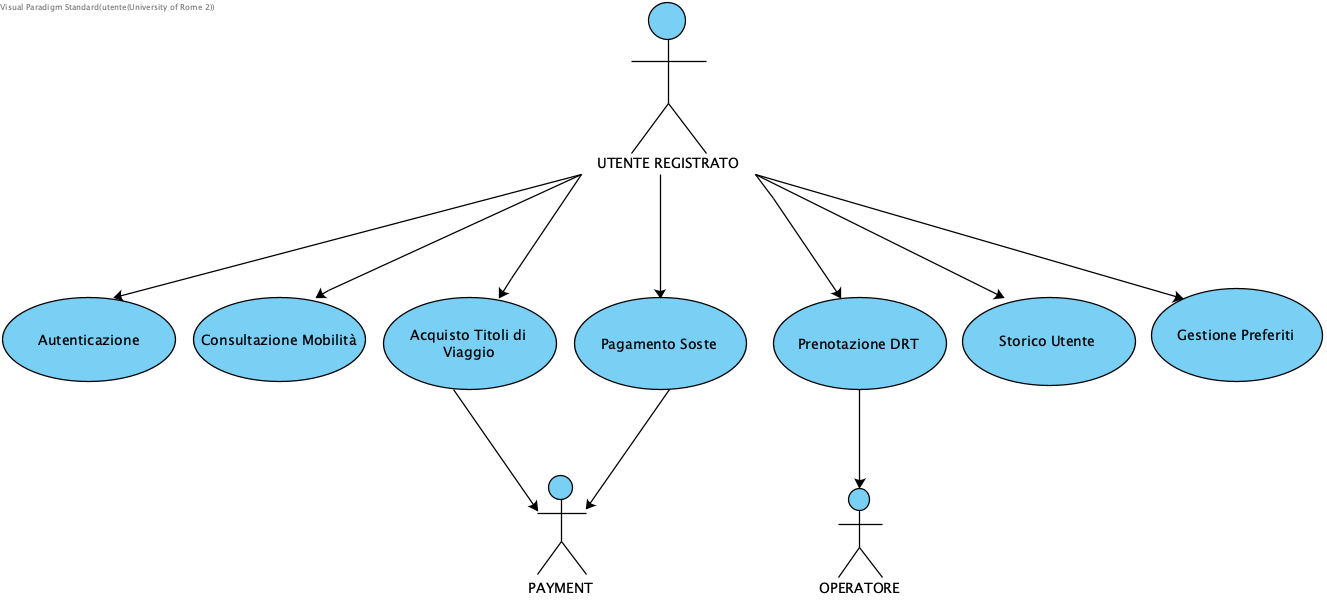
\includegraphics[width=0.9\linewidth]{UseCase/Utente_Registrato.png}
    \label{fig:placeholder}
\end{figure}
\newpage

\subsection*{Documentazione}
\addcontentsline{toc}{subsection}{Documentazione}

\begin{center}
    Use Case: Autenticazione. 
\end{center}
Il caso d'uso Autenticazione, descrive la procedura di accesso al sistema da parte dell'Utente Registato. \\
Attraverso l'autenticazione il sistema ricorda chi è l'utente, in base ai dati che ha fornito durante la Registrazione. \\
Tramite l'inserimento delle proprie credenziali, l'utente viene riconosciuto dal sistema e sblocca servizi avanzati appositamente per lui, ovvero consultare i suoi titoli di viaggio o i suoi abbonamenti, la sua cronologia, e così via.  

\vspace{0.5cm}

%TABELLA 
\usecasetable
{Autenticazione}
{Procedura di accesso al sistema tramite verifica delle credenziali.}
{Utente Registrato, Admin, Operatore, Funzionario.}
{L'utente deve possedere un account attivo.}
{1. L'utente inserisce email e password. \newline 2. Il sistema valida i dati. \newline 3. Viene garantito l'accesso al profilo.}
{1a. Credenziali errate: il sistema segnala l'errore e nega l'accesso.}
{Sessione utente avviata e accesso alle funzionalità riservate.}
\newpage
\begin{center}
    Use Case: Consultazione mobilità. 
\end{center}
Il caso d'uso Consultazione Mobilità, condiviso dai profili Turista e Utente non Registrato, consente la ricerca e la visualizzazione di informazioni relative alla rete di trasporto, permettendo all'Utente Registrato la consultazione di percorsi, orari, tratte e fermate con aggiornamenti in tempo reale. 

\vspace{0.5cm}

%TABELLA 
\usecasetable
{Consultazione mobilità}
{Ricerca di informazioni su tratte, orari e fermate con dati real-time.}
{Utente Registrato, Non Registrato, Turista.}
{Connessione al server attiva.}
{1. L'utente cerca una tratta. \newline 2. Il sistema mostra orari e percorsi disponibili.}
{1a. Dati in tempo reale non disponibili: il sistema mostra l'orario programmato.}
{Visualizzazione delle informazioni di viaggio.}
\newpage

\begin{center}
    Use Case: Acquisto Titoli di Viaggio
\end{center}
Il caso d'uso Acquisto Titoli di Viaggio consente l'acquisto di biglietti per le diverse tratte della rete. Questa funzionalità è prevista anche per il profilo Turista, ma è strettamente subordinata al completamento delle procedure di registrazione e autenticazione, configurandosi di fatto come un'azione riservata all'Utente che effettua l'autenticazione. 

\vspace{0.5cm}

%TABELLA
\usecasetable
{Acquisto Titoli di Viaggio}
{Acquisto di biglietti o abbonamenti digitali.}
{Utente Registrato, Turista, Payment.}
{Utente autenticato nel sistema.}
{1. Selezione titolo. \newline 2. Reindirizzamento al pagamento. \newline 3. Conferma transazione.}
{2a. Transazione fallita: il sistema annulla l'ordine e avvisa l'utente.}
{Titolo di viaggio disponibile nel profilo utente.}

\begin{center}
    Use Case: Prenotazione DRT.
\end{center}
Il caso d'uso Prenotazione DRT, condiviso anch'esso con il profilo del Turista, è un'azione riservata all'Utente che effettua l'autenticazione. Permette all'Utente Registrato di usufruire dei servizi \textit{Demand Responsive Transport (DRT)}, ovvero il trasporto su richiesta basato su corse a chiamata per collegare le frazioni al centro urbano durante specifiche fasce orarie. 

\vspace{0.5cm}

% TABELLA 
\usecasetable
{Prenotazione DRT}
{Richiesta di trasporto a chiamata per frazioni periferiche.}
{Utente Registrato, Turista, Operatore.}
{Utente autenticato.}
{1. Richiesta corsa. \newline 2. Accettazione dell'Operatore. \newline 3. Conferma orario.}
{2a. Rifiuto corsa: l'operatore segnala indisponibilità.}
{Corsa prenotata e inserita nell'agenda dell'operatore.}
\newpage

\begin{center}
    Use Case: Gestione preferiti
\end{center}
Il caso d'uso Gestione Preferiti consente all'utente di memorizzare i percorsi e le fermate di maggiore interesse, oltre a mantenere traccia dello storico delle transazioni passate. Questo caso d'uso è accessibile anche al profilo Turista, dopo aver effettuato il completamento delle procedure di registrazione e autenticazione.

\vspace{0.5cm}

% TABELLA 
\usecasetable
{Gestione Preferiti}
{Salvataggio e organizzazione di percorsi, fermate e tratte frequenti.}
{Utente Registrato, Turista.}
{Utente autenticato nel sistema.}
{1. Selezione di un elemento (fermata/tratta). \newline 2. Comando "Aggiungi ai preferiti". \newline 3. Conferma dell'inserimento nel profilo.}
{2a. Elemento già presente: il sistema propone la rimozione o l'aggiornamento dell'etichetta.}
{L'elemento è disponibile nella sezione "Preferiti" per un accesso rapido.}

\begin{center}
    Use Case: Storico Utente
\end{center}
Il caso d'uso Storico Utente, anch'esso condiviso con il profilo Turista, azione accessibile solo dopo aver effettuata la registrazione e l'autenticazione. Consente all'Utente Registrato di visualizzare l'elenco dei viaggi effettuati dalle transizioni passate. 

\vspace{0.5cm}

% TABELLA 
\usecasetable
{Storico Utente}
{Consultazione dell'elenco dei viaggi effettuati e delle transazioni passate.}
{Utente Registrato, Turista.}
{Utente autenticato nel sistema.}
{1. Accesso all'area personale. \newline 2. Selezione sezione "Storico". \newline 3. Visualizzazione dettagli viaggi e ricevute.}
{1a. Storico vuoto: il sistema visualizza un messaggio di assenza di dati.}
{L'utente ottiene visibilità sulle proprie attività pregresse.}
\newpage

\section{Use Case Utente Non Registrato}
Di seguito vengono analizzati i principali casi d'uso relativi all'Utente non Registrato.
\\
Ciascuna descrizione è seguita dal relativo diagramma dei casi d'uso (UML), pensato per fornire una visione d'insieme, e seguita dalla documentazione tecnica, che include tabelle strutturate per analizzare nel dettaglio le singole operazioni. 

\vspace{0.5cm}

\subsection*{Diagramma}
\addcontentsline{toc}{subsection}{Diagramma}
\begin{figure}[H]
    \centering
    \includegraphics[width=0.6\linewidth]{UseCase/Utente_non_Registrato.png}
    \label{fig:placeholder}
\end{figure}

\subsection*{Documentazione}
\addcontentsline{toc}{subsection}{Documentazione}

\begin{center}
    Use Case: Registrazione. 
\end{center}
Il caso d'uso Registrazione, descrive la procedura di accesso al sistema da parte dell'Utente non Registato. \\
Quest'ultimo deve registrarsi al sistema affinchè possa usare funzionalità e servizi aggiuntivi. \\
Per Registrarsi si necessita dell'inserimento dei seguenti dati: Nome, Cognome, Codice Fiscale (Identificativo), Residenza, Tipologia (Cittadino o Turista), e così via. 

\vspace{0.5cm}

%TABELLA 
\usecasetable
{Registrazione}
{Creazione di un nuovo profilo utente nel sistema.}
{Utente Non Registrato.}
{Disponibilità di una connessione di rete e dati anagrafici validi.}
{1. Inserimento dati (Nome, CF, Residenza). \newline 2. Invio richiesta. \newline 3. Validazione, creazione account e assegnazione tipologia account}
{1a. Utente già esistente: il sistema segnala che il Codice Fiscale è già censito.}
{Creazione del profilo e abilitazione alle funzionalità per Utente Registrato.}

\begin{center}
    Use Case: Consultazione mobilità. 
\end{center}
Il caso d'uso Consultazione Mobilità, condiviso dai profili Turista e Utente Registrato, consente la ricerca e la visualizzazione delle informazioni di base inerenti alla rete di trasporto. Nello specifico, per il solo Utente Registrato, il sistema offre un livello di accesso avanzato che include la consultazione dettagliata di percorsi, orari, tratte e fermate, integrando aggiornamenti sul servizio in tempo reale.

\vspace{0.5cm}

%TABELLA 
\usecasetable
{Consultazione Mobilità}
{Ricerca di informazioni generiche sulla rete di trasporto senza autenticazione.}
{Utente Non Registrato.}
{Nessuna.}
{1. Accesso alla home page. \newline 2. Ricerca orari o linee. \newline 3. Visualizzazione risultati pubblici.}
{1a. Servizio offline: il sistema mostra l'ultimo aggiornamento disponibile in cache.}
{Informazioni ottenute senza persistenza dei dati di ricerca.}
\newpage

\section{Use Case Turista}
Di seguito è riportata l'analisi dei principali casi d'uso che coinvolgono il profilo del Turista. \\ 
Ciascuna descrizione è fornita dal rispettivo diagramma (UML), che fornisce una visione d'insieme delle azioni, e dalla documentazione tecnica strutturata per un'analisi dettagliata delle operazioni.

\subsection*{Diagramma}
\addcontentsline{toc}{subsection}{Diagramma}
\begin{figure}[H]
    \centering
    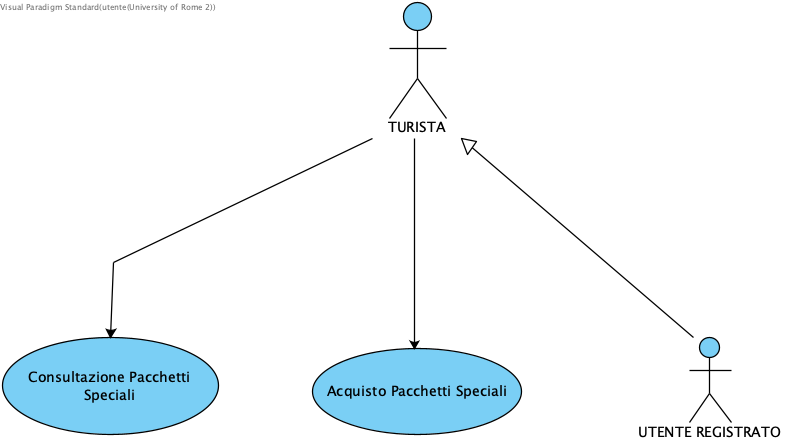
\includegraphics[width=0.7\linewidth]{UseCase/Turista.png}
    \label{fig:placeholder}
\end{figure}

\subsection*{Documentazione}
\addcontentsline{toc}{subsection}{Documentazione}

\begin{center}
    Use Case: Consultazione Pacchetti Speciali. 
\end{center}
Il caso d'uso Consultazione di Pacchetti Speciali, solamente relativo al profilo del Turista. Anch'esso vincolato al completamento delle procedure di registrazione e autenticazione. Consente al Turista di accedere  e consultare biglietti o Pacchetti Speciali per effettuare i vari spostamenti all'interno e all'esterno del comune. 

\vspace{0.5cm}

%TABELLA 
\usecasetable
{Consultazione Pacchetti Speciali}
{Visualizzazione di offerte integrate per la mobilità turistica.}
{Turista.}
{Utente autenticato come profilo "Turista".}
{1. Accesso sezione "Offerte". \newline 2. Filtro per durata o zona. \newline 3. Visualizzazione dettagli pacchetto.}
{2a. Nessun pacchetto attivo: il sistema mostra le tariffe standard.}
{Conoscenza delle opzioni di risparmio per visitatori.}
\newpage

\begin{center}
    Use Case: Acquisto Pacchetti Speciali.
\end{center}
Il caso d'uso Acquisto di Pacchetti Speciali, inerente solamente al profilo del Turista. Anch'esso vincolato al completamento delle procedure di registrazione e autenticazione. Permette al Turista di accedere ed acquistare biglietti o Pacchetti Speciali per effettuare i vari spostamenti all'interno e all'esterno del comune. 

\vspace{0.5cm}

%TABELLA 
\usecasetable
{Acquisto Pacchetti Speciali}
{Transazione economica per l'attivazione di un bundle di servizi turistici.}
{Turista, Payment.}
{Utente autenticato e metodo di pagamento valido.}
{1. Selezione pacchetto. \newline 2. Procedura di check-out. \newline 3. Validazione pagamento e attivazione.}
{3a. Errore Gateway: il sistema annulla l'operazione e ripristina lo stato precedente.}
{Pacchetto turistico associato digitalmente al profilo dell'utente.}
\newpage

\section{Use Case Admin Dell'Ente}
Passiamo ora all'analisi dei casi d'uso che riguardano l'Admin Ente. \\
Qui è presente il diagramma UML, che aiuta ad avere subito un'idea chiara delle funzionalità. \\
Subito dopo si trova la documentazione tecnica, dove attraverso delle tabelle vengono spiegate passo passo le singole operazioni.

\subsection*{Diagramma}
\addcontentsline{toc}{subsection}{Diagramma}
\begin{figure}[H]
    \centering
    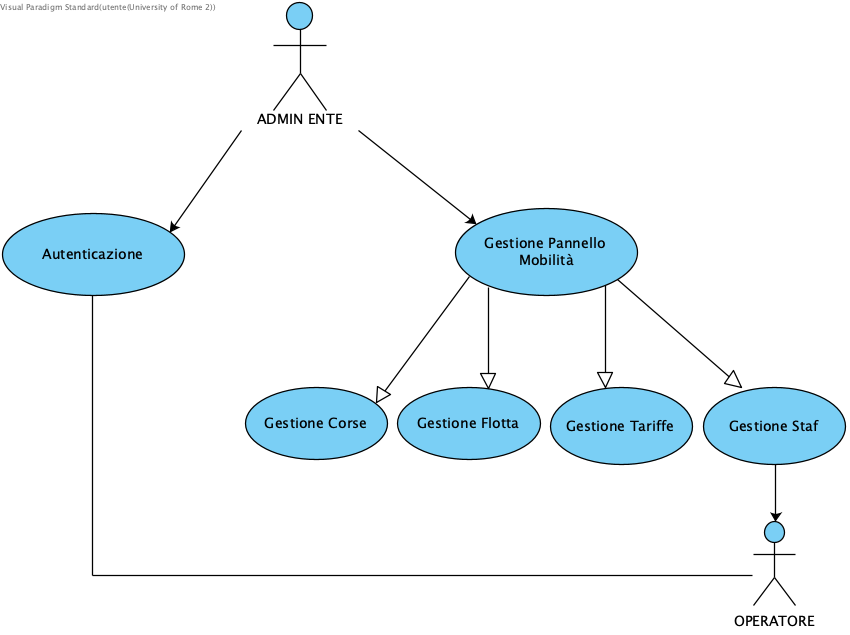
\includegraphics[width=0.7\linewidth]{UseCase/Admin_Ente.png}
    \label{fig:uc_admin_ente}
\end{figure}

\subsection*{Documentazione}
\addcontentsline{toc}{subsection}{Documentazione}

\begin{center}
    {Use Case: Autenticazione}
\end{center}
Il caso d'uso Autenticazione descrive la procedura di accesso al sistema da parte dell'Admin dell'Ente. \\
Attraverso l'autenticazione il sistema ricorda chi è l'admin, in base ai dati che ha fornito durante la Registrazione. \\
Tramite l'inserimento delle proprie credenziali, l'utente viene riconosciuto dal sistema e sblocca servizi avanzati appositamente per lui. Ovvero gestire le corse, vedere i guadagni e monitorare i mezzi.

\vspace{0.5cm}

%TABELLA
\usecasetable
{Autenticazione Admin}
{Accesso protetto al backend di gestione dell'Ente.}
{Admin Ente.}
{Possesso di credenziali amministrative.}
{1. Inserimento credenziali. \newline 2. Verifica credenziali. \newline 3. Accesso al pannello di controllo.}
{1a. Accesso negato: segnalazione di tentativo non autorizzato.}
{Accesso completo alle funzioni di configurazione sistema.}

\begin{center}
    {Use Case: Gestione Pannello Mobilità}
\end{center}
Il caso d'uso Gestione Pannello Mobilità, rappresenta l'hub centrale a cui l'Admin Ente ha accesso. Da questo pannello si diramano le funzionalità specifiche di amministrazione (corse, flotta, tariffe e staff), che costituiscono una specializzazione delle operazioni di mobilità.

\vspace{0.5cm}

%TABELLA
\usecasetable
{Gestione Pannello Mobilità}
{Hub centrale per l'amministrazione e la specializzazione delle operazioni di mobilità (corse, flotta, tariffe e staff).}
{Admin Ente.}
{L'Admin Ente deve aver effettuato l'accesso al sistema (Autenticazione completata con successo).}
{1. L'Admin accede alla dashboard principale. \newline 2. Il sistema mostra la panoramica dei servizi di mobilità. \newline 3. L'Admin seleziona l'area di interesse (es. gestione corse o flotta).}
{2a. Errore di caricamento dati: il sistema mostra un avviso e tenta una riconnessione al database.}
{L'Admin viene reindirizzato alla sezione specifica selezionata, pronto per eseguire operazioni di CRUD (Creazione, Lettura, Aggiornamento, Cancellazione).}
\newpage

\begin{center}
    {Use Case: Gestione Corse}
\end{center}
Il caso d'uso Gestione Corse, relativo solamente al profilo dell'Admin dell'Ente, permette l'inserimento delle tratte che saranno visibili all'interno del sistema.

\vspace{0.5cm}

%TABELLA
\usecasetable
{Gestione Corse}
{Modifica e programmazione delle tratte di trasporto ordinario.}
{Admin Ente.}
{Autenticazione Admin completata.}
{1. Selezione linea. \newline 2. Modifica orari o fermate. \newline 3. Pubblicazione variazioni.}
{3a. Conflitto di orari: il sistema segnala la sovrapposizione di mezzi sulla stessa tratta.}
{Database delle corse aggiornato in tempo reale per gli utenti.}

\vspace{0.5cm}

\begin{center}
    {Use Case: Gestione Flotta}
\end{center}
Il caso d'uso Gestione Flotta, anch'esso relativo solamente al profilo dell'Admin dell'Ente, permette la gestione dei mezzi, ovvero l'inserimento o la rimozione dei veicoli ad uso del Comune.

\vspace{0.5cm}

%TABELLA
\usecasetable
{Gestione Flotta}
{Amministrazione dei mezzi fisici (bus, navette) in dotazione.}
{Admin Ente.}
{Autenticazione Admin completata.}
{1. Schedatura nuovo mezzo o rimozione esistente. \newline 2. Associazione mezzo a linea. \newline 3. Salvataggio.}
{1a. ID Mezzo duplicato: il sistema richiede una matricola univoca.}
{Anagrafica flotta aggiornata e sincronizzata con la disponibilità operativa.}
\newpage

\begin{center}
    {Use Case: Gestione Tariffe}
\end{center}
Il caso d'uso Gestione Tariffe, anch'esso relativo solamente al profilo dell'Admin dell'Ente, permette all'Ente di gestire le Tariffe, consultare le entrate e le uscite, e i rimborsi.

\vspace{0.5cm}

% TABELLA
\usecasetable
{Gestione Tariffe}
{Configurazione dei prezzi e monitoraggio finanziario.}
{Admin Ente.}
{Autenticazione Admin completata.}
{1. Accesso modulo tariffe. \newline 2. Modifica prezzi o gestione rimborsi. \newline 3. Salvataggio.}
{1a. Errore dati: il sistema blocca il salvataggio di valori incongrui.}
{Parametri tariffari aggiornati nel database.}

\vspace{0.5cm}

\begin{center}
    {Use Case: Gestione Staff}
\end{center}
Il caso d'uso Gestione Staff, anch'esso relativo solamente all'Admin dell'Ente, permette la gestione degli operatori dei bus, dei controllori e di coloro che sono dipendenti dell'Ente e si trovano nella gestione dei trasporti del comune. Il sistema prevede anche un'interazione diretta con il profilo dell'Operatore, che esegue le direttive assegnate.

\vspace{0.5cm}

% TABELLA
\usecasetable
{Gestione Staff}
{Amministrazione del personale (autisti, controllori).}
{Admin Ente.}
{Autenticazione Admin completata.}
{1. Selezione dipendente. \newline 2. Assegnazione ruolo o turno. \newline 3. Aggiornamento anagrafica.}
{1a. Dipendente già assegnato: il sistema segnala il conflitto di turnazione.}
{Organico aziendale aggiornato.}
\newpage

\section{Use Case Operatore}
In questa sezione ci concentriamo sull'Operatore. \\ Anche in questo caso, è presente un diagramma UML per dare una visione d'insieme del processo. \\ A seguire, sono state riportate le tabelle tecniche per scendere nel dettaglio di come funziona esattamente ogni azione.

\subsection*{Diagramma}
\addcontentsline{toc}{subsection}{Diagramma}
\begin{figure}[H]
    \centering
    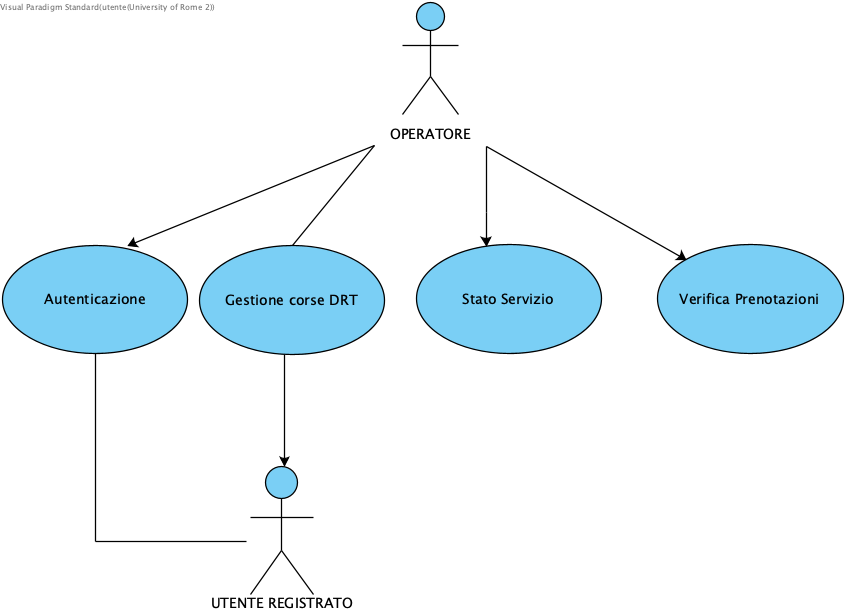
\includegraphics[width=0.7\linewidth]{UseCase/Operatore.png}
    \label{fig:placeholder}
\end{figure}

\subsection*{Documentazione}
\addcontentsline{toc}{subsection}{Documentazione}

\begin{center}
    Use Case: Autenticazione. 
\end{center}
Il caso d'uso Autenticazione, descrive la procedura di accesso al sistema da parte dell'Operatore. \\
Attraverso l'autenticazione il sistema ricorda chi è l'operatore, in base ai dati che ha fornito durante la Registrazione. \\
Tramite l'inserimento delle proprie credenziali, l'utente viene riconosciuto dal sistema e sblocca servizi appositamente per lui.

\vspace{0.5cm}

%TABELLA 
\usecasetable
{Stato Servizio}
{Aggiornamento della condizione operativa dei mezzi (in ritardo, guasto, attivo).}
{Operatore.}
{Operatore autenticato e in turno.}
{1. Selezione mezzo/corsa. \newline 2. Cambio stato (es. "In ritardo"). \newline 3. Invio aggiornamento al sistema.}
{2a. Errore di connessione: salvataggio locale e tentativo di reinvio automatico.}
{Informazione distribuita in tempo reale a tutti gli utenti del sistema.}

\begin{center}
    Use Case: Gestione Corse DRT. 
\end{center}
Il caso d'uso Gestione Corse DRT, solamente relativo al proflo dell'Operatore, permette la visione delle chiamate da parte dell'Utente Registrato o del Turista.\\  L'Operatore non solo riceve la chiamata, ma sceglie se accettare o meno la partenza della corsa.

\vspace{0.5cm}

%TABELLA 
\usecasetable
{Gestione Corse DRT}
{Validazione delle richieste di trasporto su chiamata.}
{Operatore.}
{Autenticazione Operatore completata.}
{1. Ricezione notifica chiamata. \newline 2. Valutazione logistica. \newline 3. Accettazione o rifiuto.}
{2a. Mezzi insufficienti: l'operatore declina la richiesta.}
{Aggiornamento dello stato della prenotazione lato utente.}
\newpage

\begin{center}
    Use Case: Stato Servizio.
\end{center}
Il caso d'uso Stato Servizio, anch'esso solamente relativo al profilo dell'Operatore, permette la gestione dei mezzi e degli orari, ovvero l'inserimento o l'attivazione della partenza dei mezzi disponibili.

\vspace{0.5cm}

%TABELLA 
\begin{table}[htbp]
\centering
\renewcommand{\arraystretch}{1.4}
\begin{tabular}{l p{10.5cm}}
\toprule
\textbf{Proprietà} & \textbf{Descrizione} \\
\midrule
Nome Use Case & Stato Servizio \\
Descrizione & Aggiornamento in tempo reale degli orari dei mezzi \\
Attori Coinvolti & Operatore. \\
Precondizioni & L'Operatore deve essere autenticato nel sistema e in turno. \\
Scenario Principale & 
1. Selezione del mezzo/corsa. \newline
2. Modifica dello stato.\newline
3. Conferma e invio dell'aggiornamento al sistema. \\
Scenari Alternativi & 2a. Errore di connessione: il sistema salva il dato in locale e tenta il reinvio automatico appena la rete torna disponibile. \\
Post-condizioni & Lo stato del mezzo viene aggiornato nel database e l'informazione viene distribuita in tempo reale a tutti gli utenti del sistema. \\
\bottomrule
\end{tabular}
\label{tab:uc_statoservizio}
\end{table}

\begin{center}
    Use Case: Verifica Prenotazioni.
\end{center}
Il caso d'uso Verifica Prenotazioni, anch'esso solamente relativo al profilo dell'Operatore. \\
Questa funzionalità permette la gestione delle chiamate prenotate da parte dell'Utente Registrato o del Turista.

\vspace{0.5cm}

% TABELLA 
\usecasetable
{Verifica Prenotazioni}
{Controllo della validità dei titoli di viaggio o prenotazioni DRT a bordo.}
{Operatore.}
{Operatore autenticato.}
{1. Scansione codice (QR/ID). \newline 2. Verifica nel database. \newline 3. Riscontro esito (Valido/Non Valido).}
{2a. Titolo scaduto: l'operatore invita l'utente alla regolarizzazione.}
{Validazione del diritto di accesso al mezzo di trasporto.}
\newpage

\section{Use Case Funzionario Comunale}
Vediamo adesso i casi d'uso pensati per il Funzionario Comunale. \\ Per rendere il tutto più leggibile e intuitivo, ogni funzionalità viene introdotta da uno schema UML riassuntivo. Dopodiché, la documentazione entra nello specifico con le tabelle che analizzano a fondo i vari passaggi.

\subsection*{Diagramma}
\addcontentsline{toc}{subsection}{Diagramma}
\begin{figure}[H]
    \centering
    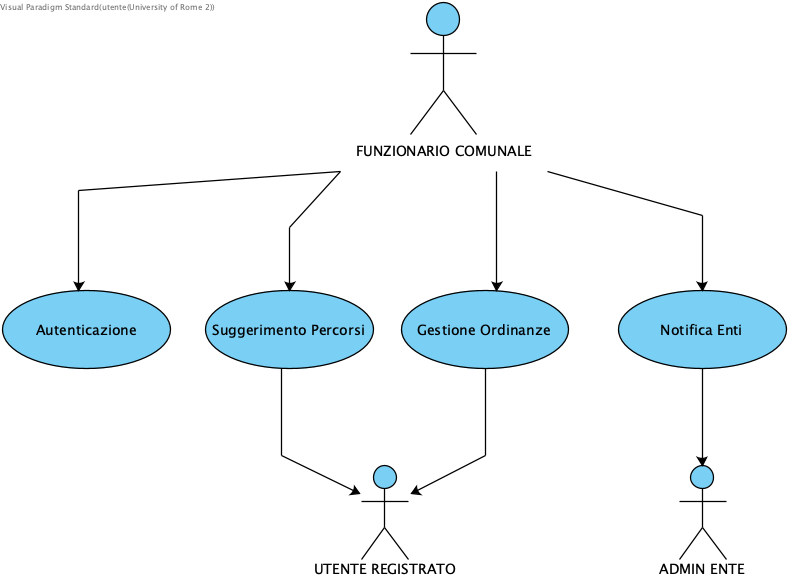
\includegraphics[width=0.7\linewidth]{UseCase/Funzionario_Comunale.png}
    \label{fig:placeholder}
\end{figure}

\subsection*{Documentazione}
\addcontentsline{toc}{subsection}{Documentazione}

\begin{center}
    Use Case: Autenticazione. 
\end{center}
Il caso d'uso Autenticazione, descrive la procedura di accesso al sistema da parte del Funzionario Comunale. \\
Attraverso l'autenticazione il sistema ricorda chi è il Funzionario Comunale, in base ai dati che ha fornito durante la Registrazione. \\
Tramite l'inserimento delle proprie credenziali, l'utente viene riconosciuto dal sistema e sblocca l'accesso a servizi appositamente per lui, più nel dettaglio, la gestione delle ordinanze di chiusura strade per eventi.

\vspace{0.5cm}

%TABELLA 
\usecasetable
{Autenticazione Funzionario}
{Accesso alle funzioni istituzionali del portale mobilità.}
{Funzionario Comunale.}
{Possesso di credenziali istituzionali.}
{1. Inserimento dati accesso. \newline 2. Validazione. \newline 3. Accesso area ordinanze e notifiche.}
{1a. Password scaduta: obbligo di rinnovo credenziali.}
{Funzionario abilitato all'inserimento di atti amministrativi.}

\begin{center}
    Use Case: Gestione Ordinanze.
\end{center}
Il caso d'uso Gestione Ordinanze, solamente relativo al profilo del Funzionario Comunale, permette l'inserimento di ordinanze rilasciate dal Comune e visibili all'interno del sistema.

\vspace{0.5cm}

%TABELLA
\usecasetable
{Gestione Ordinanze}
{Inserimento di provvedimenti comunali con impatto sulla viabilità.}
{Funzionario Comunale.}
{Autenticazione Funzionario completata.}
{1. Caricamento ordinanza. \newline 2. Definizione aree impattate. \newline 3. Invio notifiche.}
{1a. Documento non valido: il sistema richiede un formato PDF conforme.}
{Alert visibili su mappa e notifiche inviate agli enti interessati.}
\newpage

\begin{center}
    Use Case: Suggerimento Percorsi.
\end{center}
Il caso d'uso Suggerimento Percorsi, anch'esso solamente relativo al profilo del Funzionario Comunale, permette la gestione dei mezzi, ovvero le variazioni apportate ai percorsi in caso di eventi mondani.

\vspace{0.5cm}

%TABELLA 
\usecasetable
{Suggerimento Percorsi}
{Modifica dinamica dei tracciati in risposta a esigenze temporanee.}
{Funzionario Comunale.}
{Autenticazione Funzionario completata.}
{1. Identificazione area critica. \newline 2. Tracciamento percorso alternativo. \newline 3. Approvazione modifica.}
{2a. Percorso non percorribile: il sistema segnala vincoli di altezza/peso per i mezzi pesanti.}
{Ricalcolo automatico dei tempi di percorrenza e percorsi per l'utenza.}

\begin{center}
    Use Case: Notifiche Enti
\end{center}
Il caso d'uso Notifiche Enti, anch'esso solamente relativo al profilo del Funzionario Comunale. \\ 
Questa funzionalità permette a quest'ultimo di notificare agli Enti, attraverso allert automatici, deviazioni o cambiamenti sulla gestione della mobilità urbana.

\vspace{0.5cm}

% TABELLA 
\usecasetable
{Notifiche Enti}
{Comunicazione formale di variazioni della mobilità verso soggetti terzi.}
{Funzionario Comunale.}
{Autenticazione Funzionario completata.}
{1. Creazione avviso. \newline 2. Informare gli Enti \newline 3. Invio.}
{3a. Errore invio: notifica di mancata ricezione per specifici canali.}
{Enti informati e coordinati sulle variazioni del traffico urbano.}
\newpage

\section{Use Case Payment}
Infine, vengono analizzati i casi d'uso legati al Pagamento. \\ Anche qui, troviamo un diagramma UML, che ci permette di mostrare come si sviluppa il flusso. \\ 
Le tabelle che seguono servono invece a "smontare" le singole transazioni e spiegarle nel dettaglio.

\subsection*{Diagramma}
\addcontentsline{toc}{subsection}{Diagramma}
\begin{figure}[H]
    \centering
    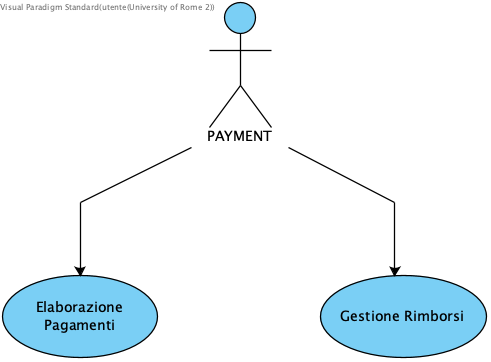
\includegraphics[width=0.6\linewidth]{UseCase/Payment.png}
    \label{fig:placeholder}
\end{figure}

\subsection*{Documentazione}
\addcontentsline{toc}{subsection}{Documentazione}

\begin{center}
    Use Case: Elaborazione Pagamenti.
\end{center}
Il caso d'uso Elaborazione Pagamenti, è solamente relativo al Payment, un attore non "umano", che gestisce i pagamenti all'interno del sistema. \\ Questa funzionalità permette al payment, attraverso un'interfaccia esterna l'elaborazione delle transizioni entranti agli Enti, in sicurezza.

\vspace{0.5cm}

%TABELLA 
\usecasetable
{Elaborazione Pagamenti}
{Gestione tecnica delle transazioni finanziarie.}
{Payment (Sistema Esterno).}
{Richiesta di acquisto avviata da un utente.}
{1. Ricezione dati transazione. \newline 2. Verifica fondi. \newline 3. Notifica esito positivo.}
{2a. Fondi insufficienti o carta scaduta: notifica errore.}
{Trasferimento fondi completato e ricevuta generata.}
\newpage

\begin{center}
    Use Case: Gestione Rimborsi.
\end{center}
Il caso d'uso Gestione Rimborsi, anch'esso solamente relativo anch'esso al Payment, permette di gestire le procedure di riborso in caso di annullamenti.

\vspace{0.5cm}

% TABELLA 
\usecasetable
{Gestione Rimborsi}
{Storno di pagamenti effettuati per servizi non usufruiti o cancellati.}
{Payment (Sistema Esterno), Admin Ente.}
{Esistenza di una transazione originale valida.}
{1. Richiesta di rimborso (automatica o manuale). \newline 2. Verifica condizioni di storno. \newline 3. Accredito fondi.}
{2a. Termini scaduti: il sistema nega il rimborso automatico.}
{Aggiornamento contabile e ripristino fondi verso l'utente.}
\newpage

\subsection*{Requisiti Funzionali}
I requisiti funzionali specificano dettagliatamente le azioni e le modalità di elaborazione dei dati che il sistema deve obbligatoriamente implementare. Sulla base degli obiettivi di digitalizzazione del contesto di Scicli, avremo i seguenti requisiti: 

\begin{table}[H]
\centering
\tiny
\renewcommand{\arraystretch}{1.4} 
\begin{tabularx}{\textwidth}{|l|l|X|X|}
\hline
\textbf{Attore} & \textbf{ID} & \textbf{Requisiti funzionali} & \textbf{Descrizione} \\ \hline

\multirow{7}{*}{Utente Registrato} & 1.1 & Autenticazione & Accede al profilo tramite credenziali per sbloccare i servizi avanzati. \\ \cline{2-4} 
 & 1.2 & Consultazione mobilità & Visualizza orari, fermate, mappe e itinerari in tempo reale. \\ \cline{2-4} 
 & 1.3 & Acquisto titoli di viaggio & Effettua l'acquisto di biglietti e abbonamenti digitali. \\ \cline{2-4} 
 & 1.4 & Prenotazione DRT & Prenota servizi di trasporto a richiesta per le frazioni e il centro. \\ \cline{2-4} 
 & 1.5 & Gestione preferiti & Salva percorsi e fermate frequenti per un accesso rapido. \\ \cline{2-4} 
 & 1.6 & Storico utente & Visualizza l'elenco dei viaggi effettuati e delle transazioni passate. \\ \cline{2-4} 
 & 1.7 & Pagamento soste & Corrisponde la tariffa per il parcheggio nelle aree a strisce blu. \\ \hline

\multirow{1}{*}{Utente Non Reg.} & 2.1 & Registrazione & Effettua una registrazione compilando un form dove inserisce un username, una password, e altri dati da utilizzare nella fase di Autenticazione \\ \cline{2-4} 
& 2.2 & Consultazione mobilità & Visualizza orari, fermate, mappe e itinerari senza necessità di registrazione. \\ \hline

% Corretto multirow a 3 perché ci sono 3 righe per il Turista
\multirow{3}{*}{Turista} & 3.1 & Consultazione Pacchetti Speciali & Consultazione di itinerari selezionati e promozioni per turisti.\\ \cline{2-4} 
 & 3.2 & Acquisto Pacchetti Speciali & Acquisto di itinerari selezionati e promozioni per turisti.\\ \hline

\multirow{5}{*}{Admin Ente} & 4.1 & Autenticazione & Accesso protetto al pannello di controllo gestionale. \\ \cline{2-4} 
 & 4.2 & Gestione corse & Crea, modifica o cancella linee, orari e frequenze dei mezzi. \\ \cline{2-4} 
 & 4.3 & Gestione flotta & Gestisce l'aggiunta o la rimozione dei mezzi monitorati. \\ \cline{2-4} 
 & 4.4 & Gestione tariffe & Configura i costi dei titoli di viaggio e le promozioni attive. \\ \cline{2-4} 
 & 4.5 & Gestione staff & Assegna gli operatori alle corse e monitora il servizio. \\ \hline

\multirow{4}{*}{Operatore} & 5.1 & Autenticazione & Accesso al pannello di controllo degli autisti. \\ \cline{2-4} 
 & 5.2 & Gestione corse DRT & Riceve e accetta le assegnazioni per il trasporto a chiamata. \\ \cline{2-4} 
 & 5.3 & Stato servizio & Segnala l'inizio, la fine o eventuali anomalie/ritardi. \\ \cline{2-4} 
 & 5.4 & Verifica prenotazioni & Visualizza la lista dei passeggeri prenotati per la tratta. \\ \hline

\multirow{4}{*}{Funzionario Comunale} & 6.1 & Autenticazione & Accesso autorizzato per la gestione della viabilità cittadina. \\ \cline{2-4} 
 & 6.2 & Gestione ordinanze & Inserisce avvisi di chiusura strade per eventi o manutenzione. \\ \cline{2-4} 
 & 6.3 & Suggerimento percorsi & Imposta deviazioni e itinerari alternativi per i mezzi. \\ \cline{2-4} 
 & 6.4 & Notifica enti & Invia alert automatici ai gestori per variazioni urgenti. \\ \hline

\multirow{2}{*}{Payment (System)} & 7.1 & Elaborazione pagamenti & Interfaccia esterna per processare le transazioni in sicurezza. \\ \cline{2-4} 
 & 7.2 & Gestione rimborsi & Gestisce le procedure di storno in caso di annullamento. \\ \hline

\end{tabularx}
\end{table}
\newpage

\subsection*{Requisiti Non Funzionali}
I requisiti non funzionali descrivono le caratteristiche qualitative, i vincoli tecnici e i livelli di servizio del software. 
\\
Per il nostro software, stabiliamo i seguenti parametri:

\begin{table}[h!]
\centering
\small
\renewcommand{\arraystretch}{1.5}
\begin{tabularx}{\textwidth}{|l|X|}
\hline
\textbf{Requisito} & \textbf{Descrizione} \\ \hline
\textbf{Performance} & Il sistema deve garantire il caricamento delle mappe e degli orari in maniera rapida per assicurare un'esperienza fluida. \\ \hline

\textbf{Scalabilità} & Il sistema deve permettere l'aggiunta di nuovi enti di trasporto e deve supportare un incremento del traffico gestito con l'integrazione di ulteriori API di mobilità (es. Google Maps Platform, TomTom API) senza richiedere una ristrutturazione del codice esistente. \\ \hline

\textbf{Portabilità} & L'applicazione, sviluppata con il framework React Native, deve garantire la piena compatibilità con i sistemi operativi Android e iOS. L'interfaccia deve adattarsi correttamente a diverse risoluzioni e dimensioni di schermo degli smartphone. \\ \hline

\textbf{Affidabilità} & Il sistema deve operare correttamente nel 99\% dei casi, garantendo la continuità dei servizi di trasporto essenziali. In caso di errore nel processo di pagamento o nella prenotazione, il software deve fornire feedback chiari e gestire il ripristino dello stato precedente per evitare perdite di dati o transazioni duplicate. \\ \hline

\textbf{Manutenibilità} & La struttura deve consentire interventi di manutenzione rapidi e l'aggiornamento semplificato dei database relativi a orari e tariffe. Il codice deve essere documentato per facilitare il passaggio di consegne e futuri sviluppi incrementali da parte dell'amministrazione comunale. \\ \hline

\textbf{Disponibilità} & Le funzionalità di mobilità devono essere operative per il 99.5\% del tempo, specialmente durante le fasce orarie di servizio dei mezzi pubblici e delle navette turistiche. Il monitoraggio delle chiusure stradali deve essere garantito h24 per fornire sempre percorsi aggiornati. \\ \hline

\textbf{Usabilità} & L'interfaccia deve essere intuitiva per un pubblico eterogeneo (residenti e turisti). Il design deve supportare la multilingua (italiano/inglese). L'obiettivo è minimizzare il tasso di errore dell'utente durante le varie  prenotazioni. \\ \hline

\textbf{Sicurezza} & La gestione dei dati sensibili, della cronologia degli spostamenti e delle transazioni finanziarie deve essere protetta tramite crittografia. L'accesso alle funzionalità di gestione (Admin Ente e Funzionario) deve essere regolato da un sistema di autenticazione robusto per prevenire accessi non autorizzati. \\ \hline
\end{tabularx}
\end{table}
\newpage

\chapter{Progettazione del Sistema}
Al fine di garantire una corretta memorizzazione delle informazioni e l'esecuzione di query efficienti in tempo reale, l'architettura del sistema viene modellata seguendo un approccio \textit{orientato agli oggetti (OO).} 

%INSERISCI CLASS DIAGRAM 
\section*{Class Diagram }
\addcontentsline{toc}{section}{Class Diagram}
In particolare, il Diagramma delle Classi (\textit{Class Diagram}) definisce l'architettura statica del software secondo i paradigmi della \textit{programmazione Object-Oriented (OOP)}. All'interno di tale diagramma vengono strutturate le classi relative alla gestione dei vari profili d'accesso presenti nel sistema.
\begin{figure}[H]
    \centering
    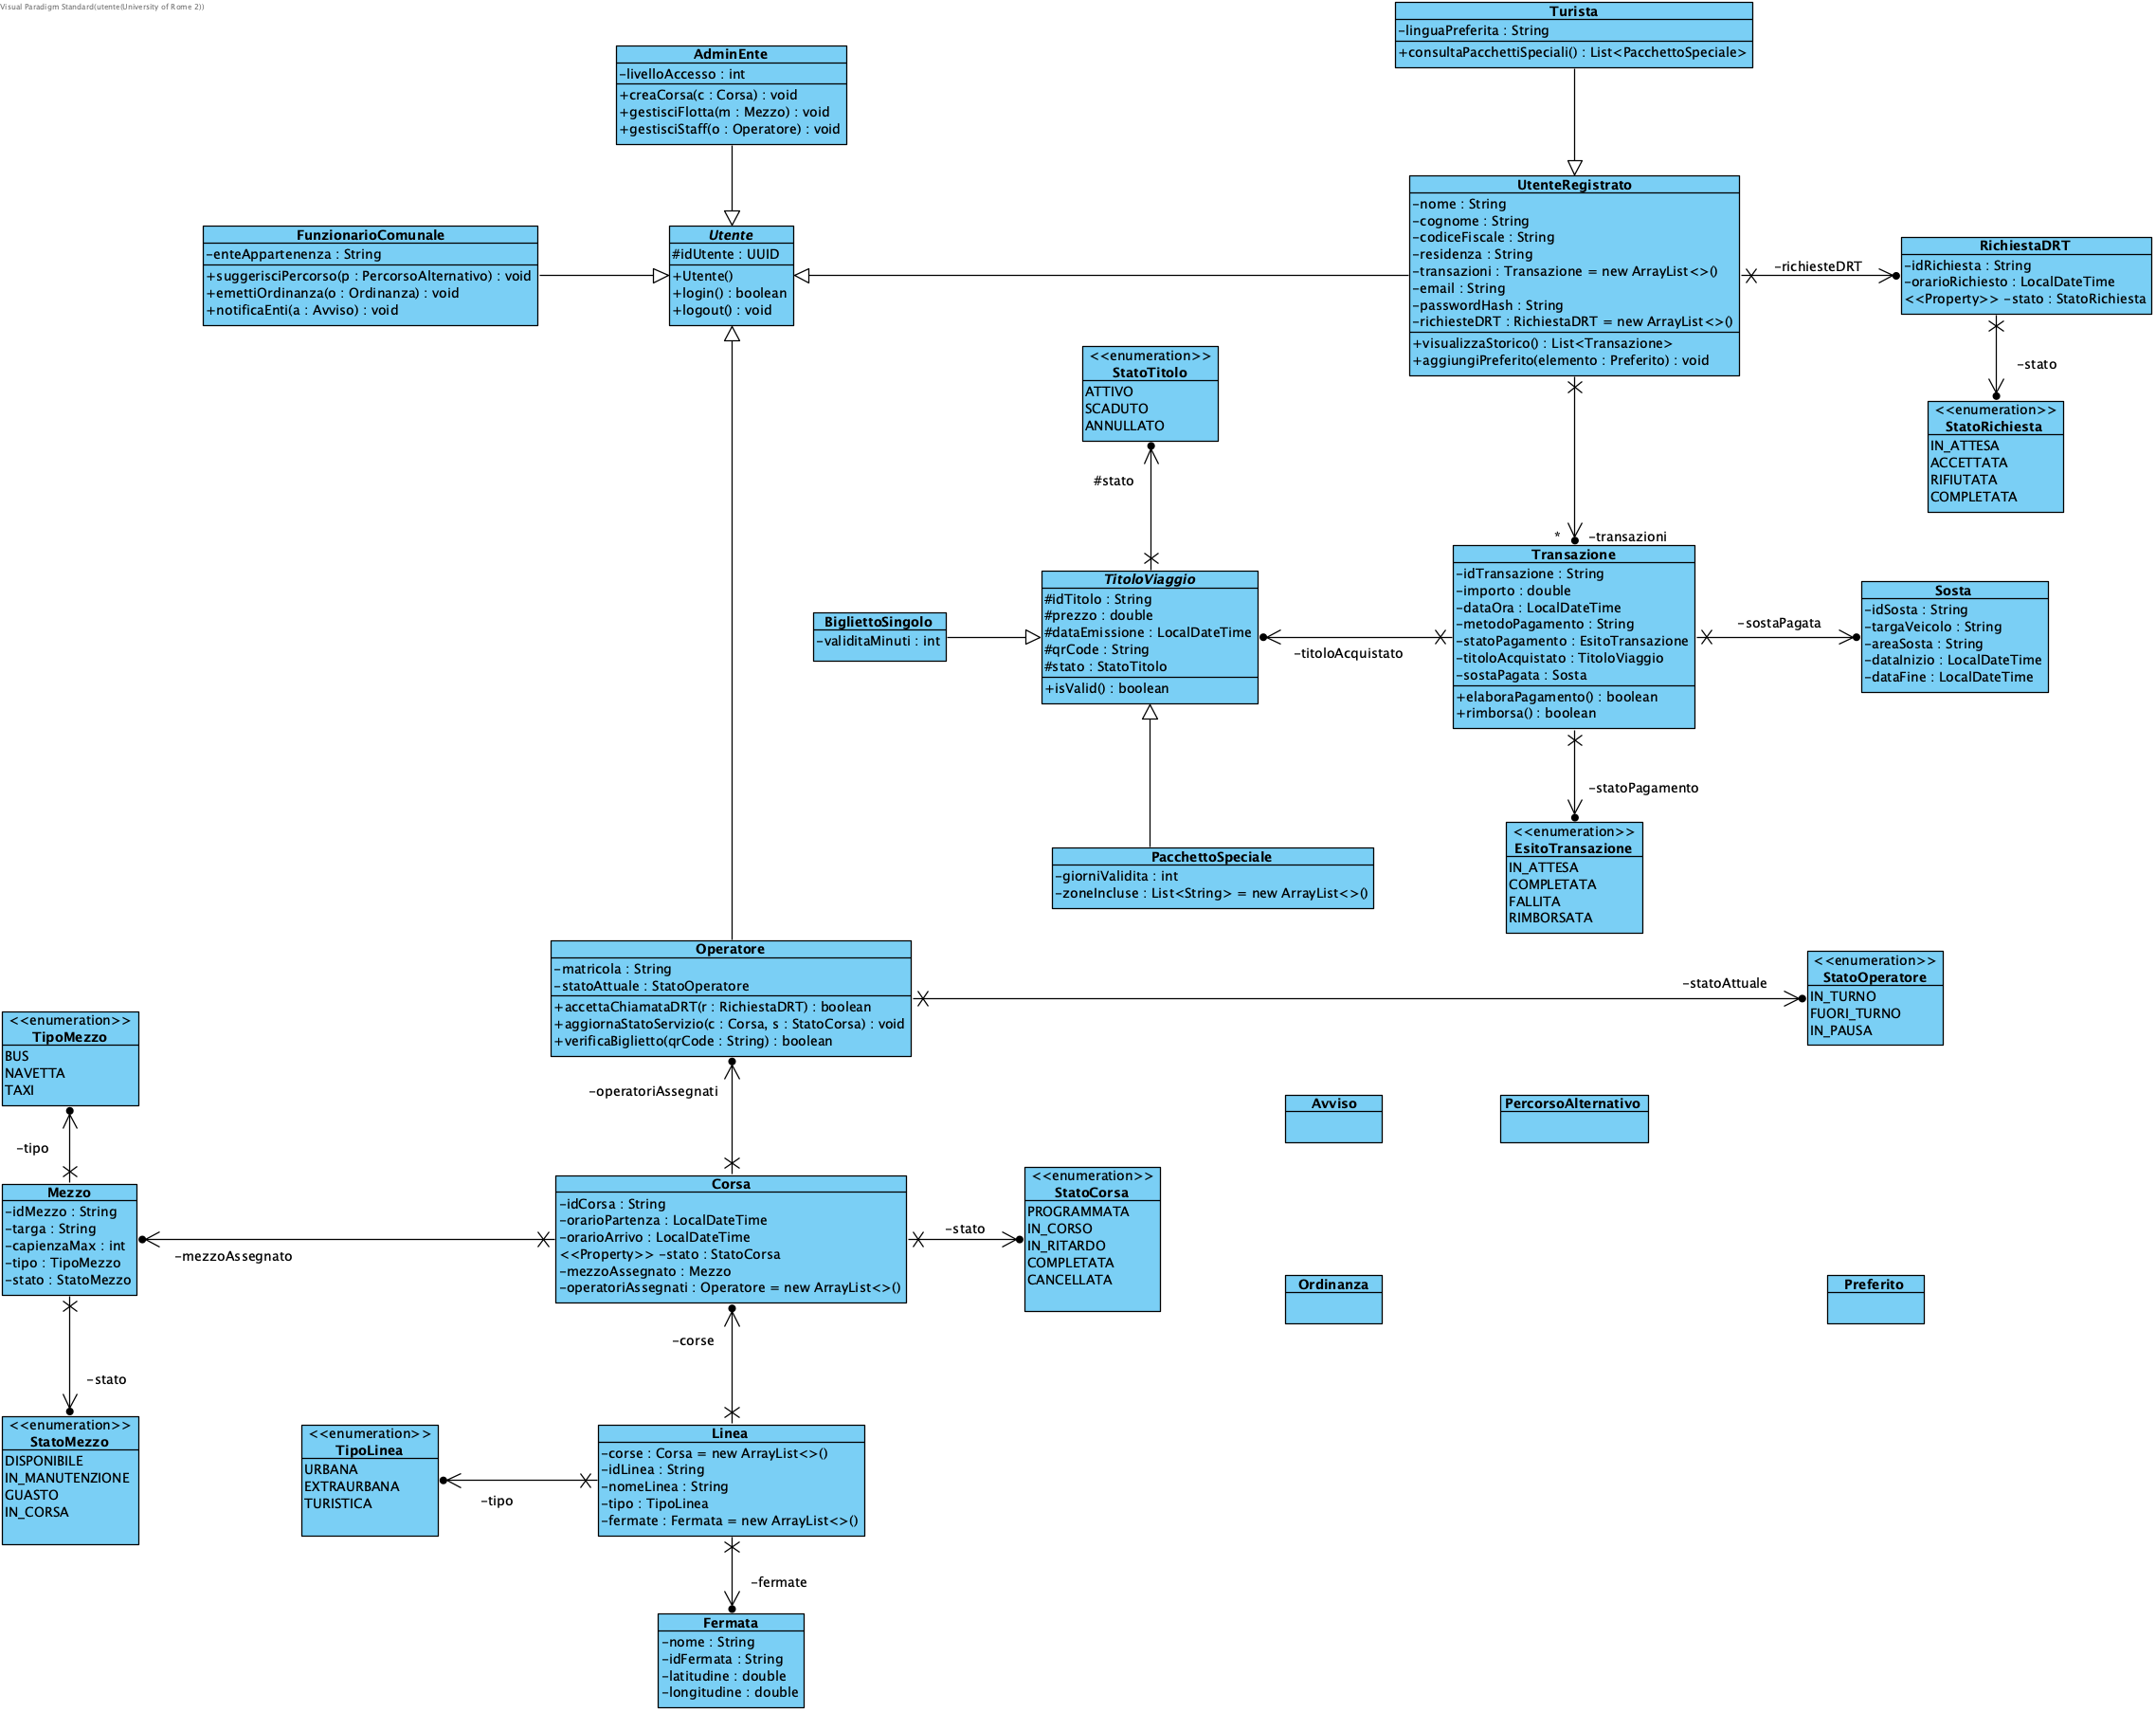
\includegraphics[width=\linewidth]{Class Diagram/Class Diagram4.png}
    \caption{}
    \label{fig:placeholder}
\end{figure}

%INSERISCI ACTIVITY DIAGRAM 
\newpage
\section*{Activity Diagram }
\addcontentsline{toc}{section}{Activity Diagram}
Infine, studiamo i \textit{diagrammi di attività} (detti anche \textit{Activity Diagram}). \\
Questi vengono utilizzati per descrivere le singole fasi dei processi interni più complessi. Nel nostro scenario, l'activity diagram modellerà il comportamento del sistema attraverso molteplici contesti operativi. Per rendere l'analisi più chiara e strutturata, ho deciso di suddividere la modellazione dei flussi di lavoro in base ai principali attori che interagiscono con la piattaforma e ai moduli di sistema più critici.

% SEZIONE UTENTE REGISTRATO

\subsection*{Azioni dell'Utente Registrato}
Il primo attore preso in esame è l'Utente Registrato. \\ Questo attore, è colui che andrà ad usare il software frequentemente per i propri spostamenti quotidiani. \\
Il suo ingresso nel sistema è regolato dal flusso di autenticazione e recupero credenziali, modellato in Figura \ref{fig:ur_auth}.

\begin{figure}[H]
    \centering
    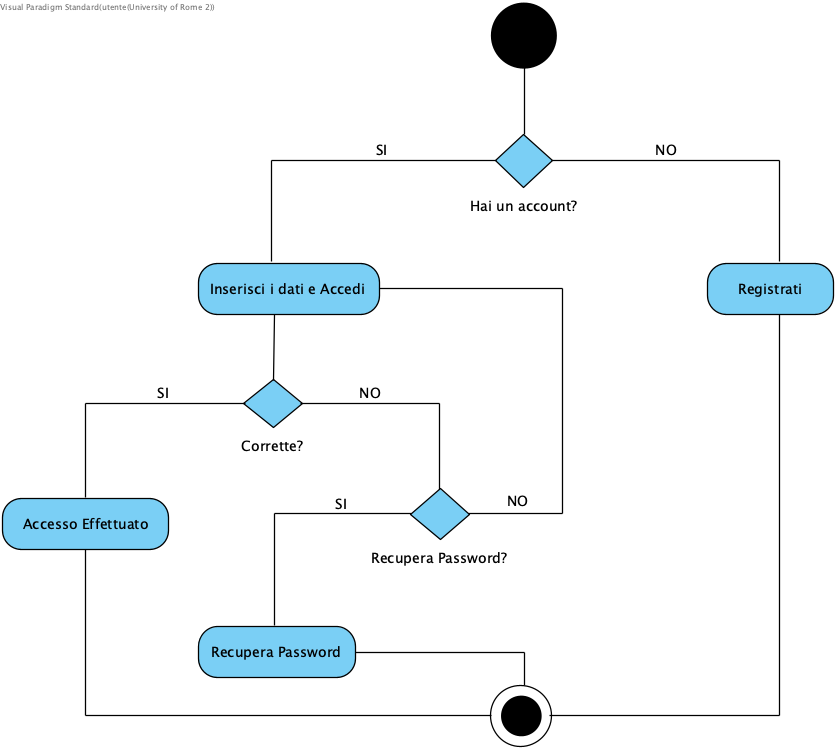
\includegraphics[width=0.8\textwidth]{Activity Diagram/Utente_Registrato/Utente_Registrato_(Autenticazione).png}
    \caption{}
    \label{fig:ur_auth}
\end{figure}
\vspace{1em}
\noindent
Una delle operazioni più frequenti compiute da questo utente è la ricerca di percorsi. \\ Accedendo al portale, egli può inserire i parametri di viaggio desiderati e avviare una ricerca iterativa fino all'individuazione di una soluzione valida (Figura \ref{fig:ur_mobilita}). A supporto di questa funzionalità, ho inserito una logica di salvataggio (Figura \ref{fig:ur_preferiti}): l'utente può aggiungere o rimuovere le tratte abituali nell'area Preferiti, migliorando notevolmente l'usabilità del software.
\begin{figure}[H]
    \centering
    \begin{minipage}{0.3\textwidth}
        \centering
        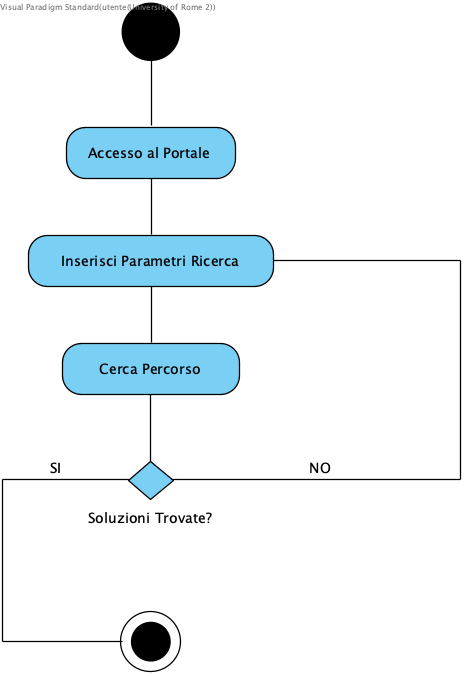
\includegraphics[width=\textwidth]{Activity Diagram/Utente_Registrato/Utente_Registrato_(Consulta MObilità).png}
        \caption{}
        \label{fig:ur_mobilita}
    \end{minipage}\hfill
    \begin{minipage}{0.6\textwidth}
        \centering
        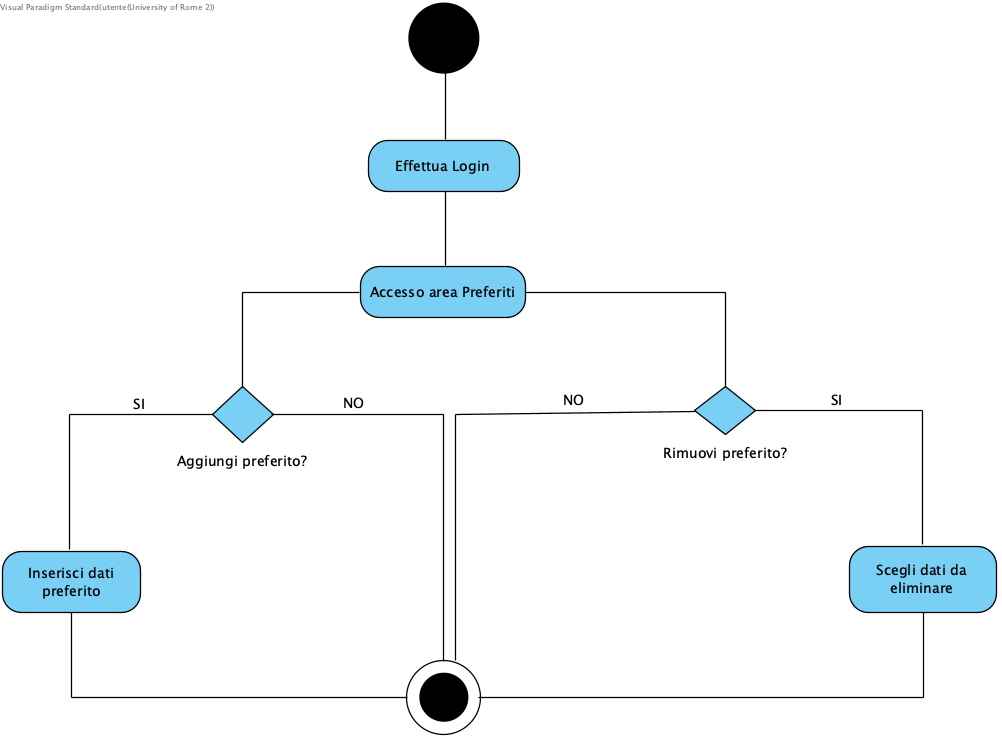
\includegraphics[width=\textwidth]{Activity Diagram/Utente_Registrato/Utente_Registarto_(Gestione_Preferiti).png}
        \caption{}
        \label{fig:ur_preferiti}
    \end{minipage}
\end{figure}
\noindent
L'applicativo gestisce in modo fluido anche i pagamenti per la sosta e il trasporto. \\ Nei diagrammi \ref{fig:ur_pag_biglietto} e \ref{fig:ur_pag_sosta} ho analizzato due scenari di acquisto molto simili ma concettualmente separati: l'acquisto di un normale biglietto (selezionando il titolo, i dati e il metodo di pagamento) e il pagamento per la sosta del proprio veicolo.
\begin{figure}[H]
    \centering
    \begin{minipage}{0.35\textwidth}
        \centering
        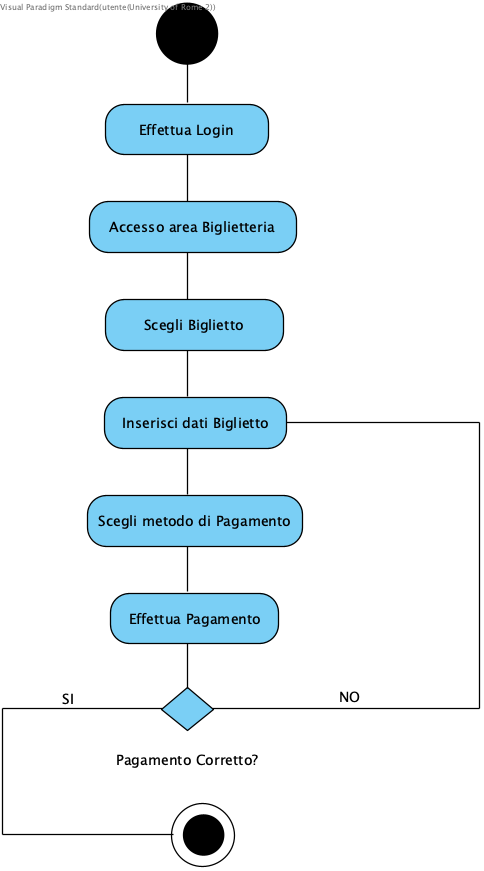
\includegraphics[width=\textwidth]{Activity Diagram/Utente_Registrato/Utente_Registrato_(Pagamento_Biglietto).png}
        \caption{}
        \label{fig:ur_pag_biglietto}
    \end{minipage}\hfill
    \begin{minipage}{0.35\textwidth}
        \centering
        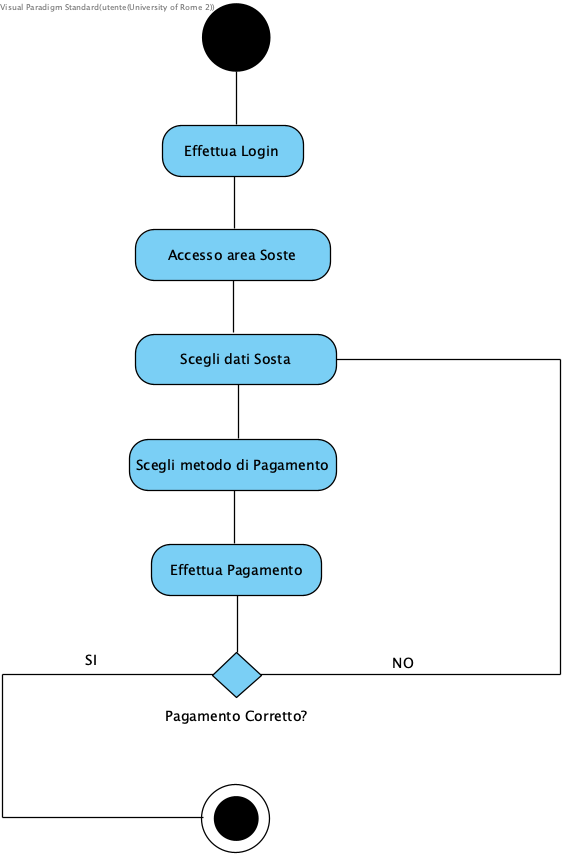
\includegraphics[width=\textwidth]{Activity Diagram/Utente_Registrato/Utente_Registrato_(Pagamento_Sosta).png}
        \caption{}
        \label{fig:ur_pag_sosta}
    \end{minipage}
\end{figure}
\noindent
Un'altra caratteristica, innovativa e molto importante che ha un impatto positivo sull'ambiente, è la prenotazione del servizio DRT (Trasporto a Chiamata). Come evidenziato in Figura \ref{fig:ur_drt}, dopo aver inserito i parametri e trovato una soluzione compatibile, l'utente seleziona le opzioni ed effettua la chiamata effettiva verso l'operatore.
\begin{figure}[H]
    \centering
    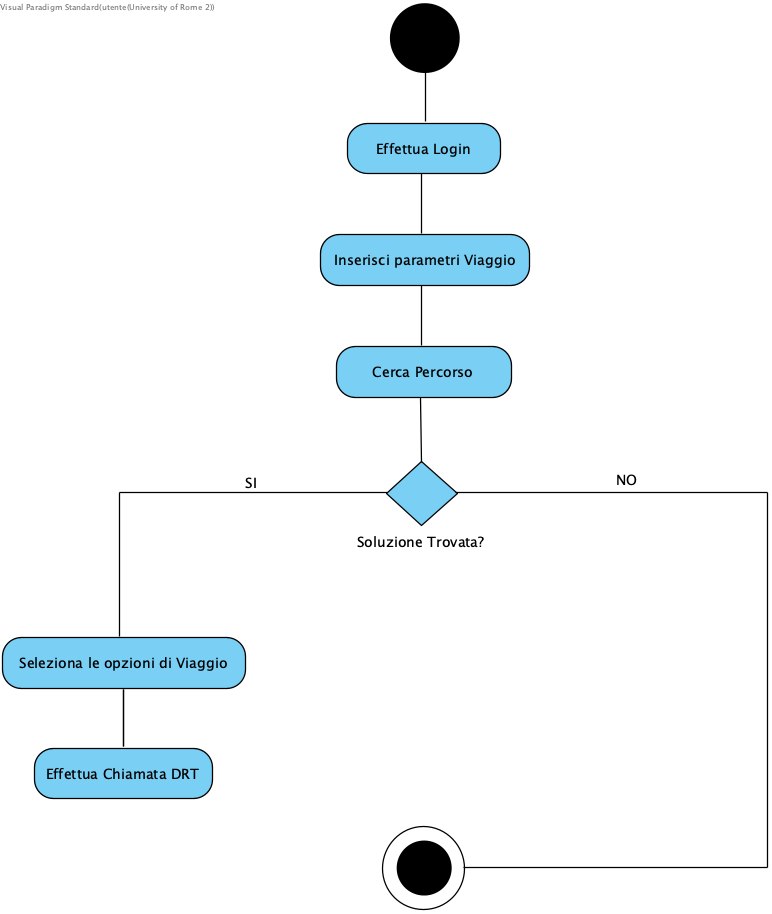
\includegraphics[width=0.45\textwidth]{Activity Diagram/Utente_Registrato/Utente_Registrato_(Prenotazione_DRT).png}
    \caption{}
    \label{fig:ur_drt}
\end{figure}
\noindent
Per concludere l'analisi di questo attore, ho modellato in Figura \ref{fig:ur_storico} la consultazione dello storico: accedendo all'area Cronologia, l'utente ha la possibilità di avere un resoconto chiaro e immediato di tutti i propri viaggi passati.
\begin{figure}[H]
    \centering
    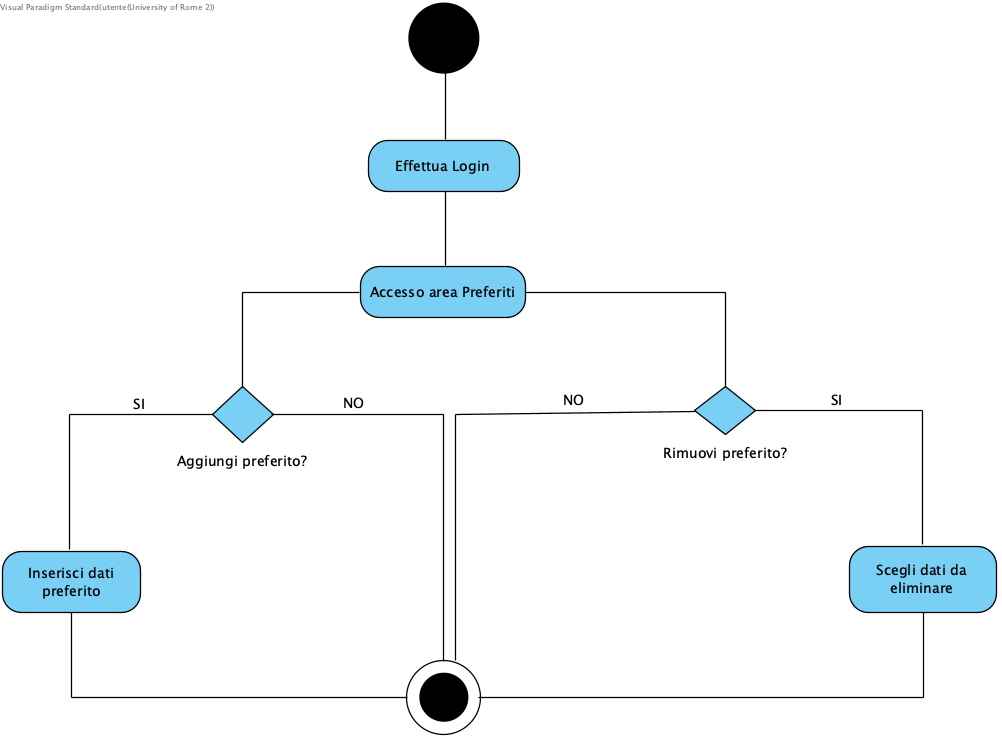
\includegraphics[width=0.6\textwidth]{Activity Diagram/Utente_Registrato/Utente_Registarto_(Gestione_Preferiti).png}
    \caption{}
    \label{fig:ur_storico}
\end{figure}

\newpage
% SEZIONE UTENTE NON REGISTRATO
\subsection*{Azioni dell'Utente Non Registrato}
A seguire, ho ritenuto opportuno descrivere anche il comportamento dell'utente il quale naviga sulla piattaforma senza possedere un account. \\
L'utente non registrato ha un accesso limitato, ma può comunque usufruire di alcune funzionalità per disporre in parte del servizio, come la consultazione della mobilità. \\ Come illustrato in Figura \ref{fig:unreg_mobilita}, il visitatore accede al portale, inserisce i parametri di ricerca e il sistema valuta iterativamente se esistono soluzioni di viaggio conformi ai criteri immessi.
\begin{figure}[H]
    \centering
    \includegraphics[width=0.25\textwidth]{Activity Diagram/Utente_non_Registrato/Utente_non_Registrato_(Consulta MObilità) copia.png}
    \caption{}
    \label{fig:unreg_mobilita}
\end{figure}
\noindent
Qualora l'utente decidesse di voler sfruttare tutte le potenzialità del sistema può attivare il processo di registrazione (Figura \ref{fig:unreg_registrazione}). Il flusso prevede la compilazione di un form e un ciclo di verifica fino alla corretta sottomissione dei dati.
\begin{figure}[H]
    \centering
    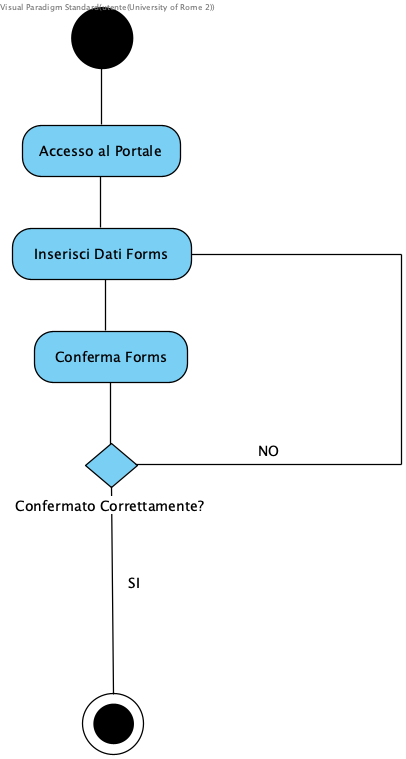
\includegraphics[width=0.25\textwidth]{Activity Diagram/Utente_non_Registrato/Utente_non_Registrato_(Registrazione).png}
    \caption{}
    \label{fig:unreg_registrazione}
\end{figure}
\newpage
% SEZIONE TURISTA
\subsection*{Azioni del Turista}
L'ultimo attore che usa il software come "consumatore" è il Turista. \\ Una volta effettuato l'accesso, l'interesse principale di questo attore è esplorare l'offerta di mobilità dedicata e acquistare i titoli di viaggio. Il flusso di consultazione è estremamente lineare: come mostrato in Figura \ref{fig:turista_consultazione}, l'utente accede all'area biglietteria ed esamina i pacchetti speciali disponibili.
\begin{figure}[H]
    \centering
    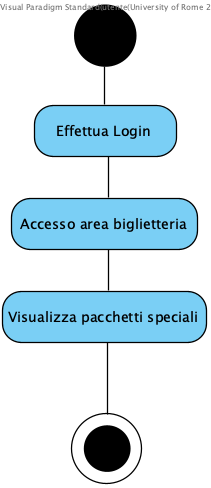
\includegraphics[width=0.2\textwidth]{Activity Diagram/Turista/Turista_(Consultazione_pacchetti).png}
    \caption{}
    \label{fig:turista_consultazione}
\end{figure}
\vspace{1em}
\noindent
Se il turista decide di procedere con l'acquisto di un pacchetto, il diagramma di attività si espande (Figura \ref{fig:turista_acquisto}). Dopo aver selezionato il pacchetto di interesse, l'utente procede all'inserimento dei dati di fatturazione fino al raggiungimento di un esito positivo della transazione.
\begin{figure}[H]
    \centering
    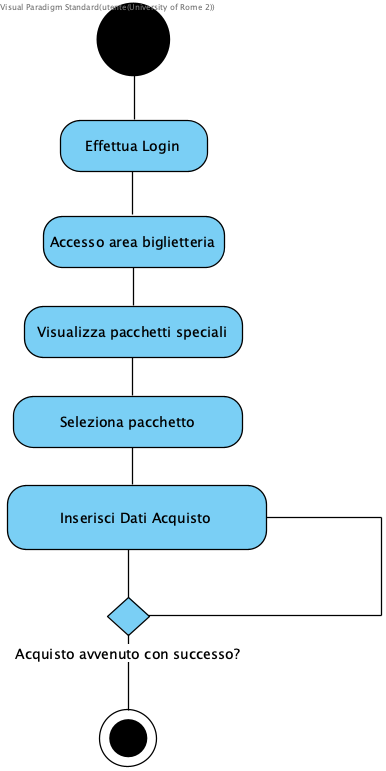
\includegraphics[width=0.25\textwidth]{Activity Diagram/Turista/Turista_(Acquista_Pacchetti).png}
    \caption{}
    \label{fig:turista_acquisto}
\end{figure}
\newpage
% SEZIONE ADMIN ENTE
\subsection*{Azioni dell'Admin Ente}
Spostandoci ora sul lato gestionale della piattaforma, analizziamo l'Admin dell'Ente. \\ Come per ogni utente del sistema, il primo passo fondamentale è l'autenticazione. Il diagramma in Figura \ref{fig:admin_auth} mostra il flusso decisionale che porta al login, alla registrazione o al recupero della password in caso di credenziali errate.
\begin{figure}[H]
    \centering
    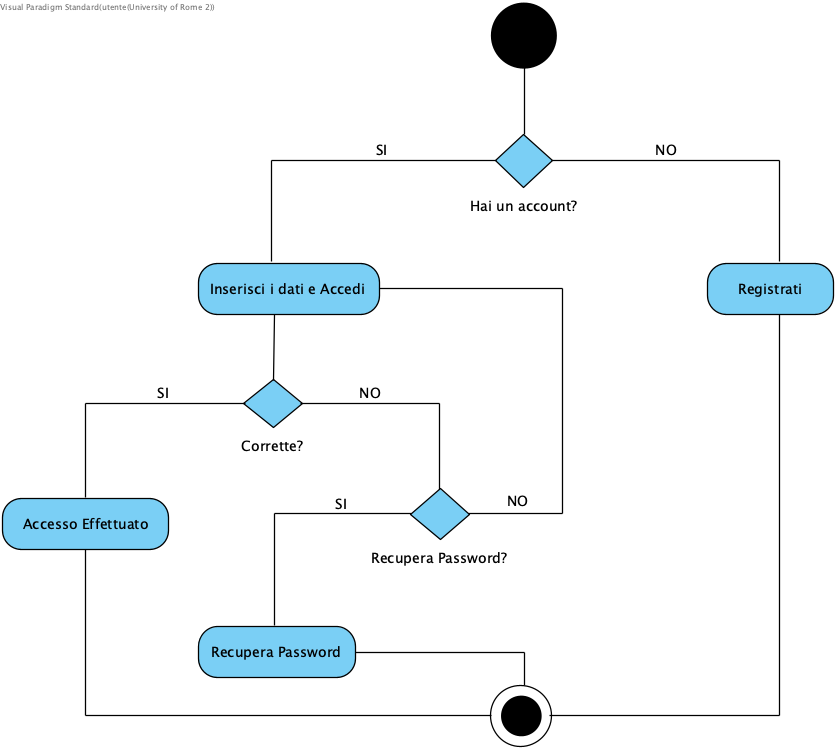
\includegraphics[width=0.5\textwidth]{Activity Diagram/Admin_Ente/Admin_Ente_(Autenticazione).png}
    \caption{}
    \label{fig:admin_auth}
\end{figure}
\noindent
Una volta effettuato l'accesso, l'Admin accede al Pannello di Mobilità. \\ Come illustrato in Figura \ref{fig:admin_pannello}, da questo snodo centrale l'utente può diramarsi in quattro attività principali: la gestione delle corse, della flotta, delle tariffe e dello staff. Ogni operazione prevede una fase di salvataggio e la possibilità di tornare al pannello principale per avviare una nuova attività.
\begin{figure}[H]
    \centering
    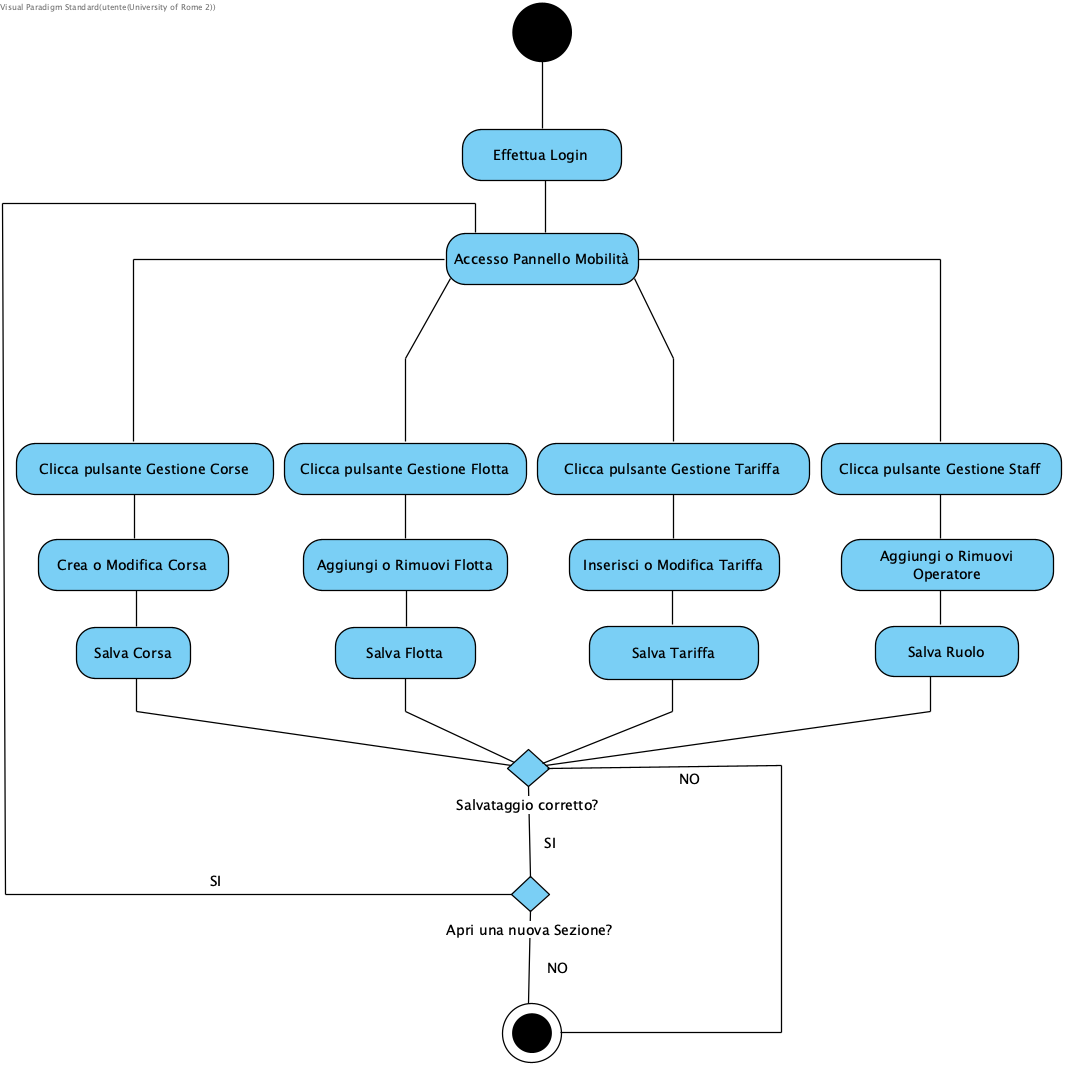
\includegraphics[width=0.5\textwidth]{Activity Diagram/Admin_Ente/Admin_Ente_(Gestione_Pannello_Mobilità).png}
    \caption{}
    \label{fig:admin_pannello}
\end{figure}
\newpage
% SEZIONE OPERATORE
\subsection*{Azioni dell'Operatore}
Un altro attore chiave della componente gestionale e operativa sul campo è l'Operatore, il quale interagisce con la piattaforma per le proprie mansioni quotidiane. Il suo flusso di autenticazione segue la logica standard del sistema (Figura \ref{fig:op_auth}).
\begin{figure}[H]
    \centering
    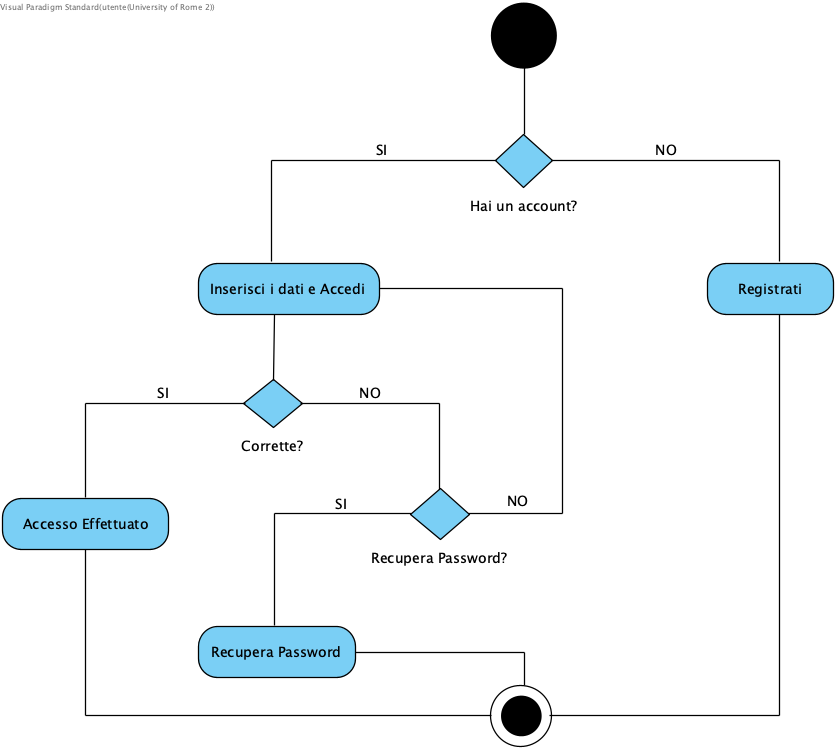
\includegraphics[width=0.5\textwidth]{Activity Diagram/Operatore/Operatore_(Autenticazione).png}
    \caption{}
    \label{fig:op_auth}
\end{figure}
\noindent
Nel contesto dei servizi di trasporto a chiamata (DRT), l'operatore riceve notifiche per nuove corse. Come vediamo in Figura \ref{fig:op_drt} vi è una semplice diramazione logica tra l'accettazione o il rifiuto della chiamata da parte dell'autista.
\begin{figure}[H]
    \centering
    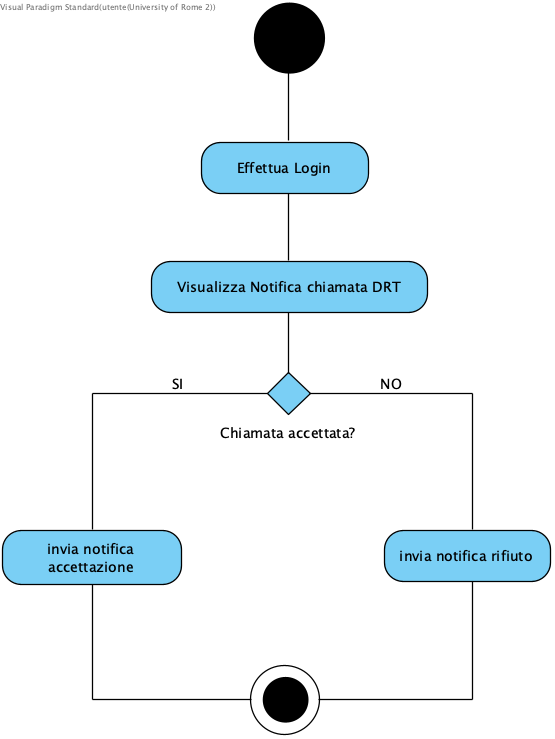
\includegraphics[width=0.3\textwidth]{Activity Diagram/Operatore/Operatore_(Gestione corse_DRT).png}
    \caption{}
    \label{fig:op_drt}
\end{figure}
\noindent
Una delle azioni più importanti dell'Operatore è quella di mantenere aggiornato lo stato del servizio. L'Activity Diagram in Figura \ref{fig:op_stato} mostra il processo ciclico di inserimento e caricamento dei dati aggiornati nell'area di servizio.
\begin{figure}[H]
    \centering
    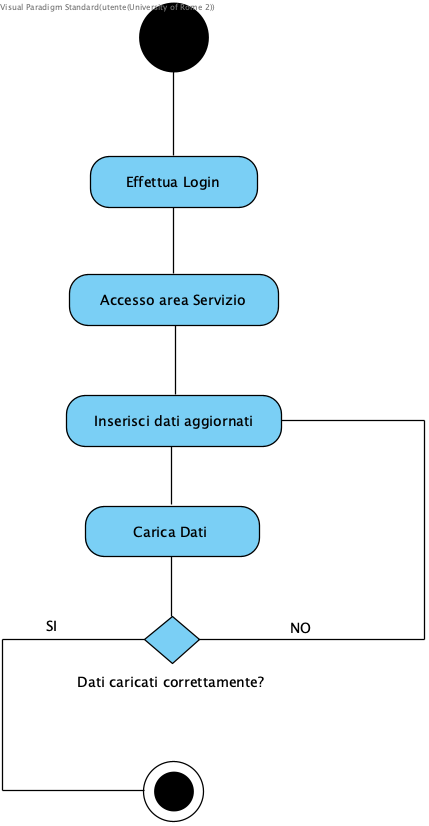
\includegraphics[width=0.3\textwidth]{Activity Diagram/Operatore/Operatore_(Stato_Servizio).png}
    \caption{}
    \label{fig:op_stato}
\end{figure}
\noindent
L'ultima azione, non per importanza, è la verifica dei titoli di viaggio. Come si evince dalla Figura \ref{fig:op_verifica}, l'operatore scannerizza il QRCode del biglietto. Se la lettura fallisce o il codice non è valido visivamente, il sistema offre un flusso alternativo permettendo l'inserimento manuale del codice.
\begin{figure}[H]
    \centering
    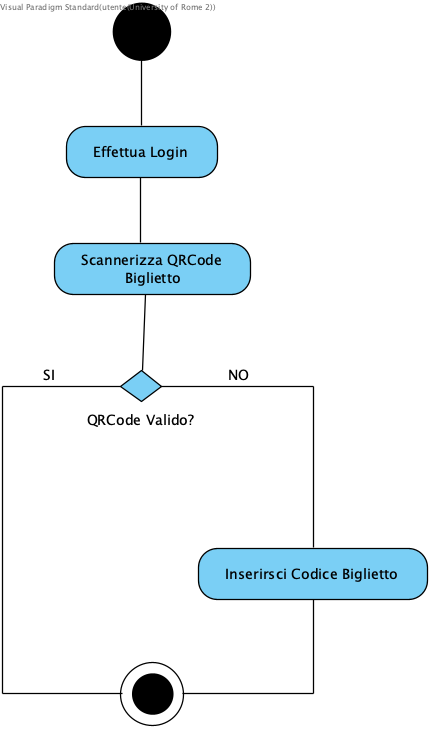
\includegraphics[width=0.3\textwidth]{Activity Diagram/Operatore/Operatore_(Verifica_Prenotazioni).png}
    \caption{}
    \label{fig:op_verifica}
\end{figure}
\newpage
% SEZIONE FUNZIONARIO COMUNALE
\subsection*{Azioni del Funzionario Comunale}
L'ultima figura che gestisce, stavolta dal punto di vista istituzionale, il software è il  Funzionario Comunale. Quest'ultimo ha un ruolo legato alla gestione degli avvisi e della viabilità cittadina. Il flusso parte regolarmente con l'autenticazione al portale (Figura \ref{fig:funz_auth}).
\begin{figure}[H]
    \centering
    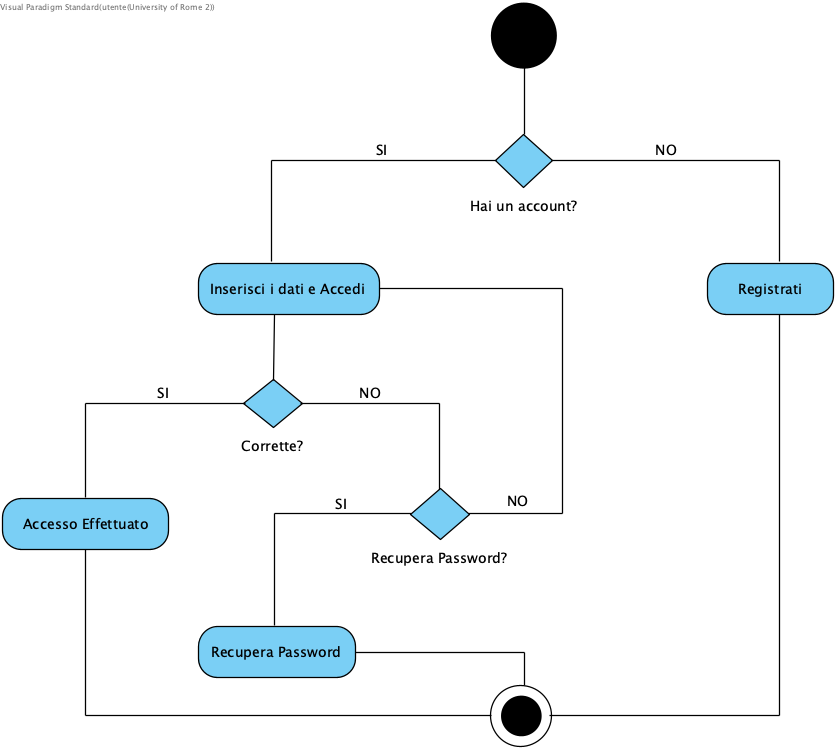
\includegraphics[width=0.5\textwidth]{Activity Diagram/Funzionario_Comunale/Funzionario_Comunale_(Autenticazione).png}
    \caption{}
    \label{fig:funz_auth}
\end{figure}
\noindent
Il funzionario ha accesso alla sezione Avvisi, dove può compiere diverse operazioni cruciali per la viabilità. La prima è la gestione delle ordinanze (Figura \ref{fig:funz_ordinanze}), che prevede il caricamento del documento e la verifica del corretto inserimento a sistema.\\
Un'altra operazione fondamentale è la comunicazione con altri enti. Come visibile in Figura \ref{fig:funz_notifica}, il funzionario può selezionare un avviso personale, scegliere l'ente destinatario, comporre un messaggio e inviarlo, con un controllo sull'esito della trasmissione.
\begin{figure}[H]
    \centering
    \begin{minipage}{0.2\textwidth}
        \centering
        \includegraphics[width=\textwidth]{"Activity Diagram/Funzionario_Comunale/Funzionario_Comunale_(Gestisce_Ordinanze).png"}
        \caption{}
        \label{fig:funz_ordinanze}
    \end{minipage}
    \hspace{3cm} 
    \begin{minipage}{0.2\textwidth}
        \centering
        \includegraphics[width=\textwidth]{"Activity Diagram/Funzionario_Comunale/Funzionario_Comunale_(Notifica_Enti).png"}
        \caption{}
        \label{fig:funz_notifica}
    \end{minipage}
\end{figure}
\noindent
Infine, per minimizzare l'impatto sul traffico durante gli eventi paesani, il funzionario può suggerire percorsi alternativi. Il diagramma in Figura \ref{fig:funz_percorsi} illustra l'inserimento dei dati relativi all'evento e il caricamento dei tracciati alternativi a sistema.
\begin{figure}[H]
    \centering
    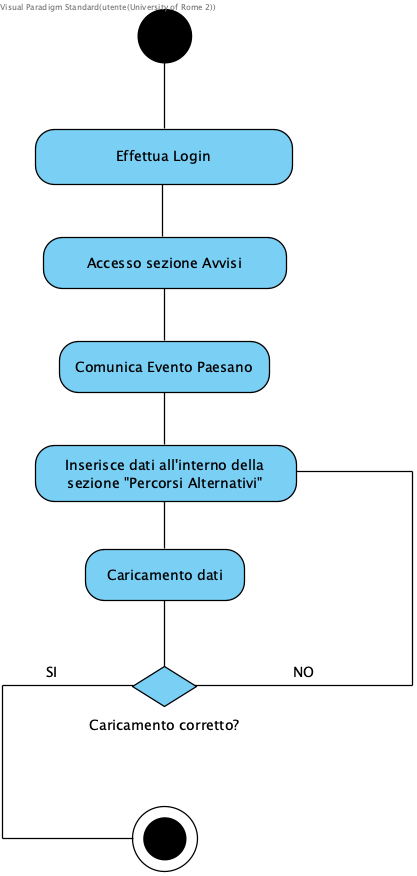
\includegraphics[width=0.4\textwidth]{Activity Diagram/Funzionario_Comunale/Funzionario_Comunale_(Suggerimento_Percorsi).png}
    \caption{}
    \label{fig:funz_percorsi}
\end{figure}
\newpage
% SEZIONE PAGAMENTI E RIMBORSI
\subsection*{Azioni del Payment}
Infine, per garantire la robustezza logica dell'intera applicazione, ho studiato i flussi relativi al modulo delle transazioni finanziarie. A differenza dei precedenti, questi diagrammi coinvolgono attivamente il backend e sistemi di terze parti (modellati tramite le \textit{partitions}). \\
La Figura \ref{fig:pay_elaborazione} mostra il processo di elaborazione dei pagamenti: il sistema riceve e controlla il formato dei dati; in caso di esito positivo, richiede l'autorizzazione a un modulo esterno o ente bancario e, all'arrivo della risposta di approvazione, aggiorna il database ed emette la ricevuta.
\begin{figure}[H]
    \centering
    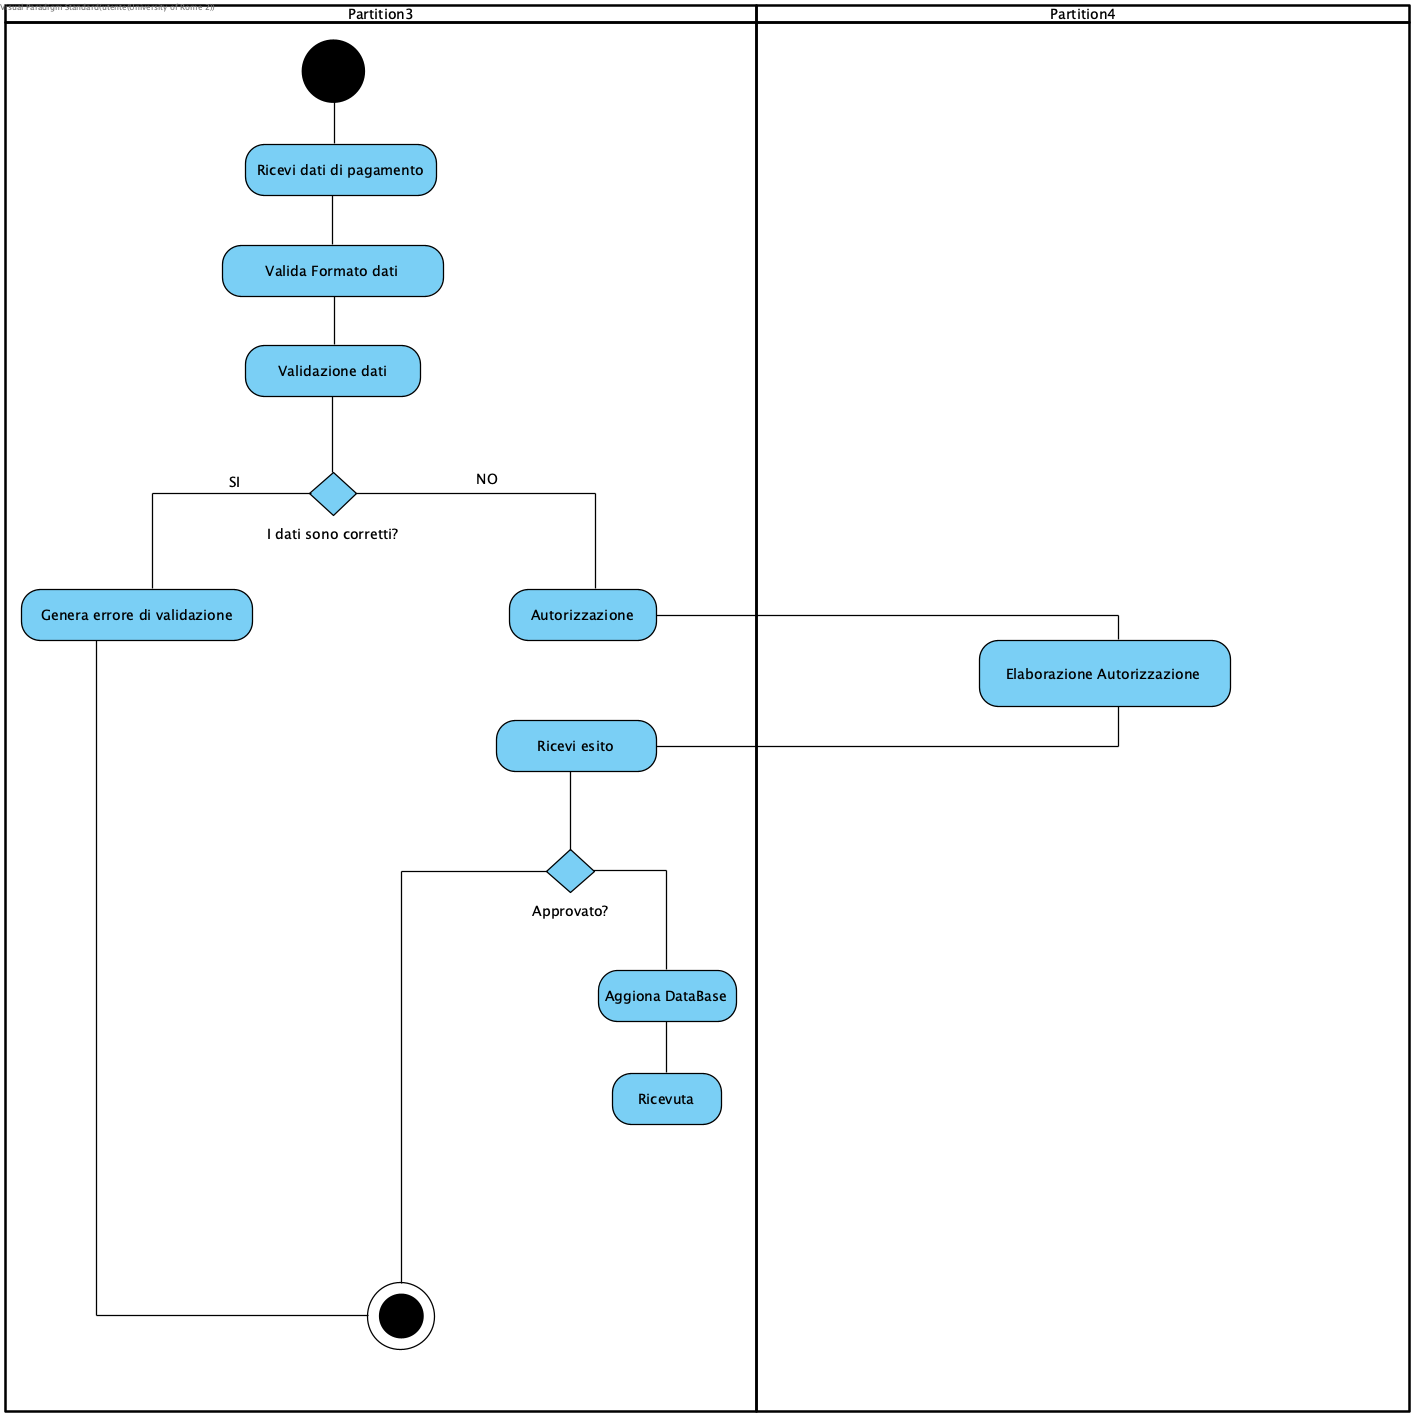
\includegraphics[width=0.4\textwidth]{Activity Diagram/Payment/Payment_(Elaborazione_Pagamenti).png}
    \caption{}
    \label{fig:pay_elaborazione}
\end{figure}
\noindent
Parallelamente, anche la gestione dei rimborsi (Figura \ref{fig:pay_rimborsi}) segue un iter di validazione rigoroso e cross-partition. A seguito di una richiesta, il sistema recupera la transazione, verifica i criteri di idoneità per il reso e, in caso positivo, elabora lo storno.
\begin{figure}[H]
    \centering
    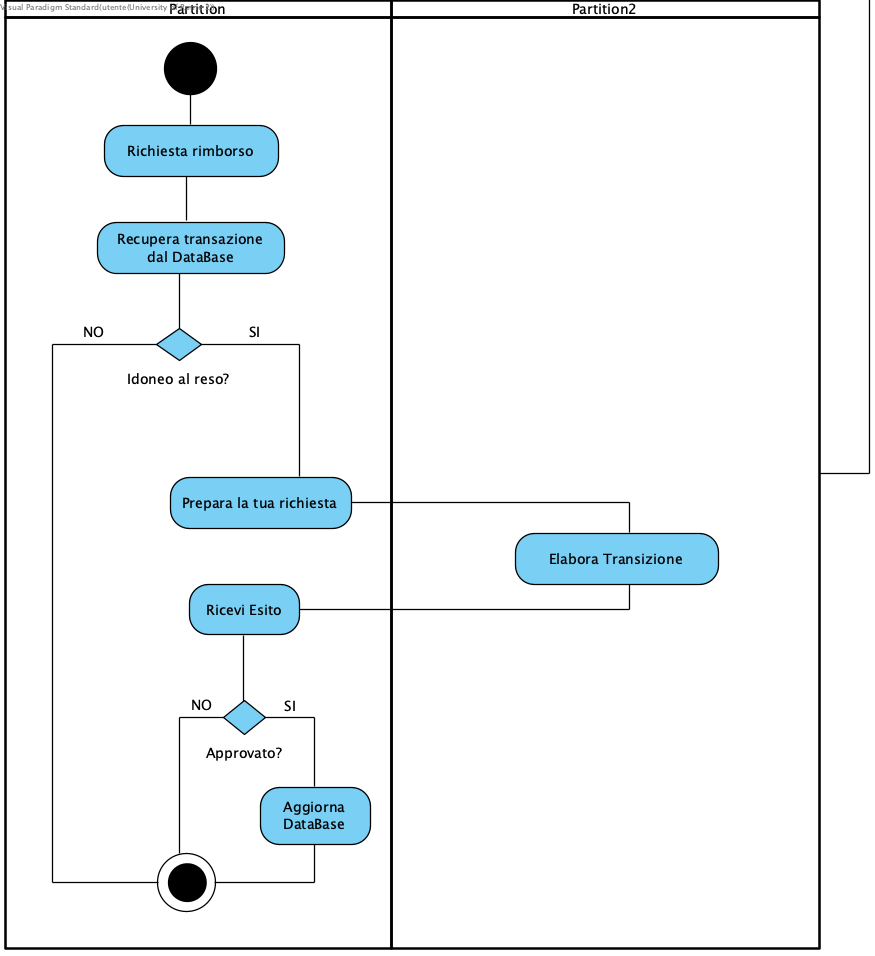
\includegraphics[width=0.4\textwidth]{Activity Diagram/Payment/Payment_(Gestione_RImborsi).png}
    \caption{}
    \label{fig:pay_rimborsi}
\end{figure}

%INSERISCI SEQUENCE DIAGRAM 
\newpage
\section*{Sequence Diagram }
\addcontentsline{toc}{section}{Sequence Diagram}
Successivamente, andremo ad analizzare i \textit{diagrammi di sequenza} (detti anche \textit{sequence diagram}).
\\
Questi catturano l'evoluzione temporale dei messaggi e delle richieste di metodi scambiati tra i vari oggetti e attori del sistema. 

% SEZIONE UTENTE REGISTRATO
\subsection*{Sequence dell'Utente Registrato}
Di seguito vengono presentati i Sequence Diagram relativi alle principali operazioni effettuate dall'attore \textbf{Utente Registrato}. Questi schemi illustrano in dettaglio come le richieste dell'utente vengano gestite dai vari componenti del sistema.
\\
Il primo processo analizzato riguarda proprio l'autenticazione, in cui l'utente inserisce le proprie credenziali, come visibile nella Figura \ref{fig:ur_auth}. Le credenziali vengono validate dal sistema: in caso di successo viene garantito l'accesso, mentre in caso di fallimento viene notificata l'assenza dell'account o avviata la procedura per il recupero della password.

\begin{figure}[H]
    \centering
    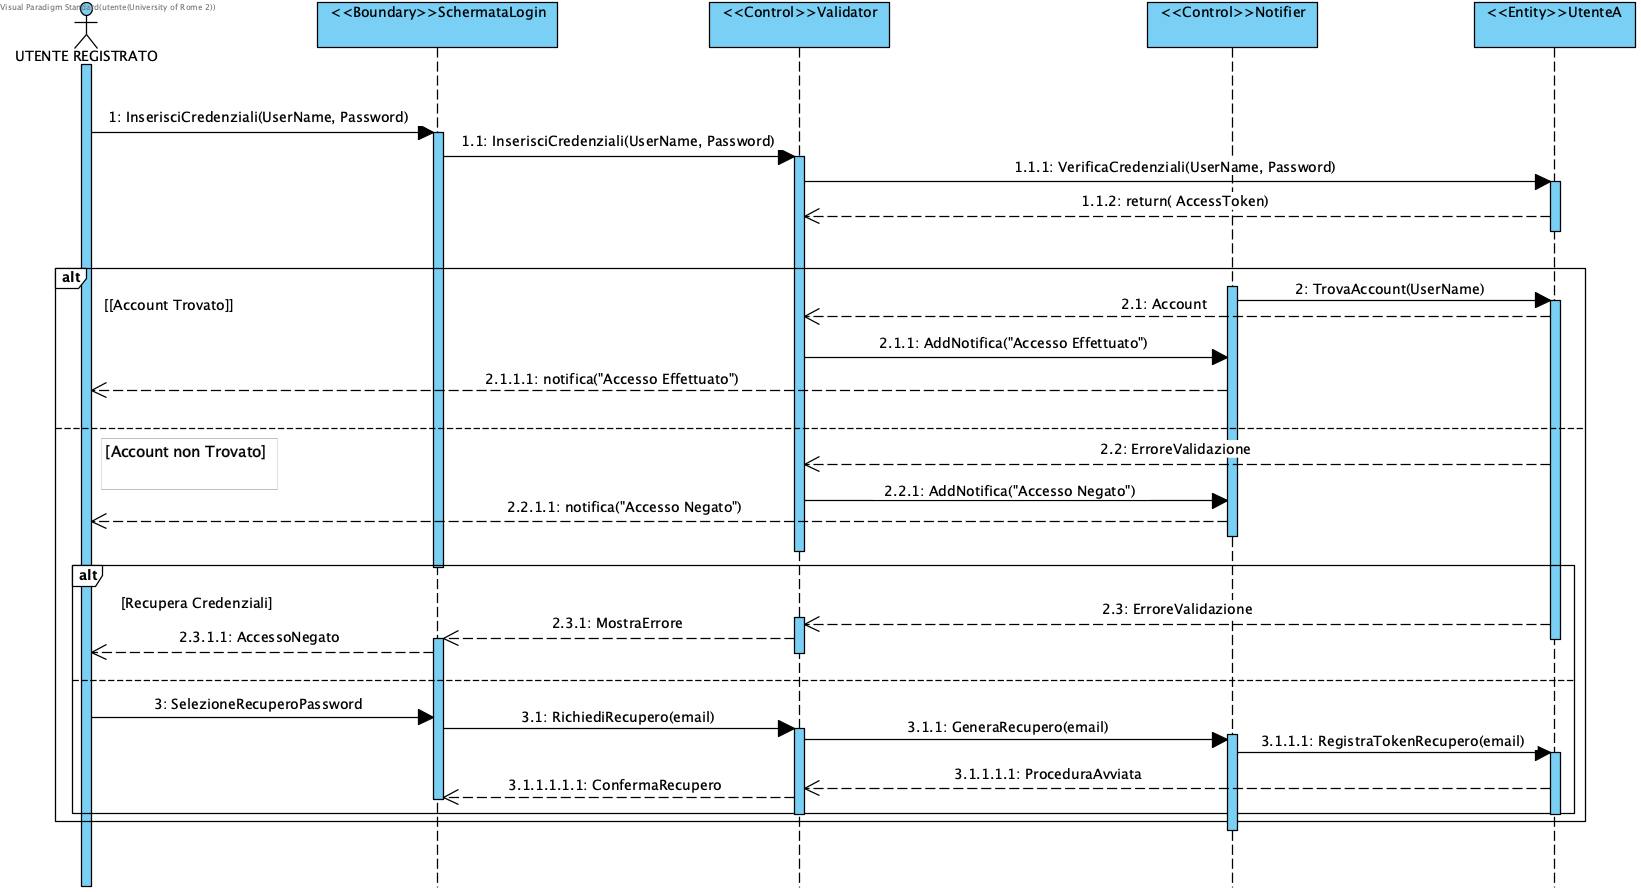
\includegraphics[width= 1.0\textwidth]{Sequence Diagram/Utente_Registrato_(Autenticazione).png}
    \caption{}
    \label{fig:ur_auth}
\end{figure}
\newpage

\noindent Una volta autenticato, l'utente può interagire con le funzionalità principali, tra cui la consultazione della mobilità. 
La seguente procedura riguarda la ricerca di una tratta (Figura \ref{fig:seq_cons}) prevedendo l'inserimento dei parametri di partenza e destinazione; se ritenuti validi dai moduli di controllo, il sistema restituisce le informazioni dettagliate su tratte, orari, fermate e stato del servizio, altrimenti richiede una correzione manuale all'utente.

\begin{figure}[H]
    \centering
    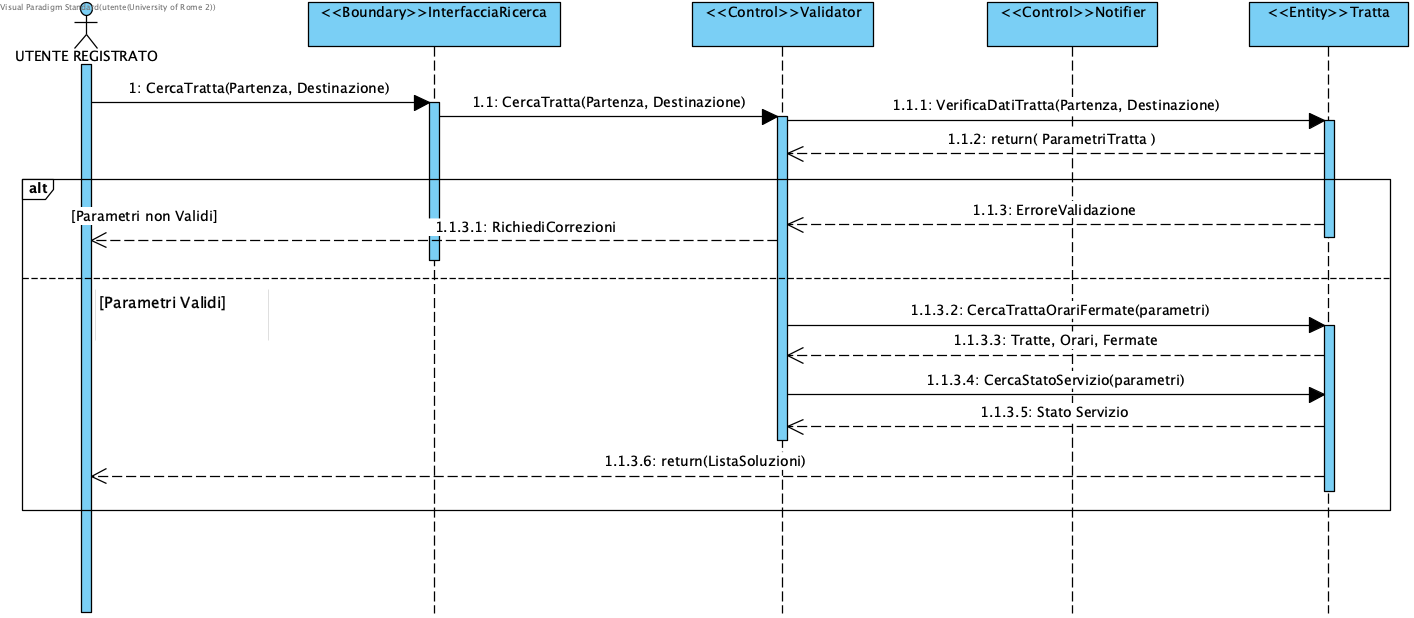
\includegraphics[width=1.0\textwidth]{Sequence Diagram/Utente_Registrato_(Consultazione_Mobilità).png}
    \caption{}
    \label{fig:seq_cons}
\end{figure}

\noindent Per agevolare l'utilizzo continuativo dell'applicazione, il sistema offre la possibilità di salvare percorsi e fermate ricorrenti. Il diagramma in Figura \ref{fig:seq_pref} mostra come l'utente possa aggiungere o rimuovere specifici elementi interfacciandosi con la schermata dedicata, la quale mantiene all'interno del sistema le tratte preferite dall'utente.

\begin{figure}[H]
    \centering
    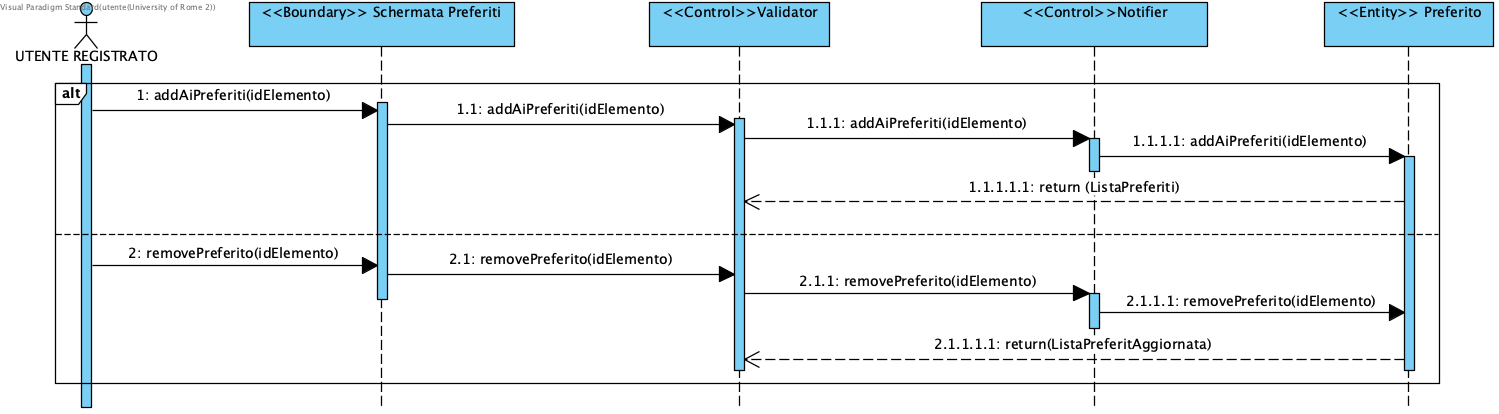
\includegraphics[width= 1.0\textwidth]{Sequence Diagram/Utente_Registro_(Gestione_Preferiti).png}
    \caption{}
    \label{fig:seq_pref}
\end{figure}
\newpage

\noindent Un aspetto cruciale dell'infrastruttura riguarda la gestione delle transazioni economiche, suddivise nell'acquisto di titoli di viaggio e nel pagamento delle soste. Nel caso dell'acquisto di un biglietto (Figura \ref{fig:seq_ticket}), il sistema elabora e valida i dati di pagamento interagendo in back-end con i componenti di controllo, generando infine una ricevuta se l'operazione va a buon fine, oppure richiedendo di modificare i dati in caso di errore.
\\
Similmente, per il pagamento di un'area di sosta, come evidenziato nella Figura \ref{fig:seq_soste}, vediamo come i dati in ingresso differiscono dal precedente sequence (infatti i nuovi dati sono: targa, orari, area specifica), ma la validazione e la notifica dell'esito della transazione mantengono la medesima coerenza architetturale.

\begin{figure}[H]
    \centering
    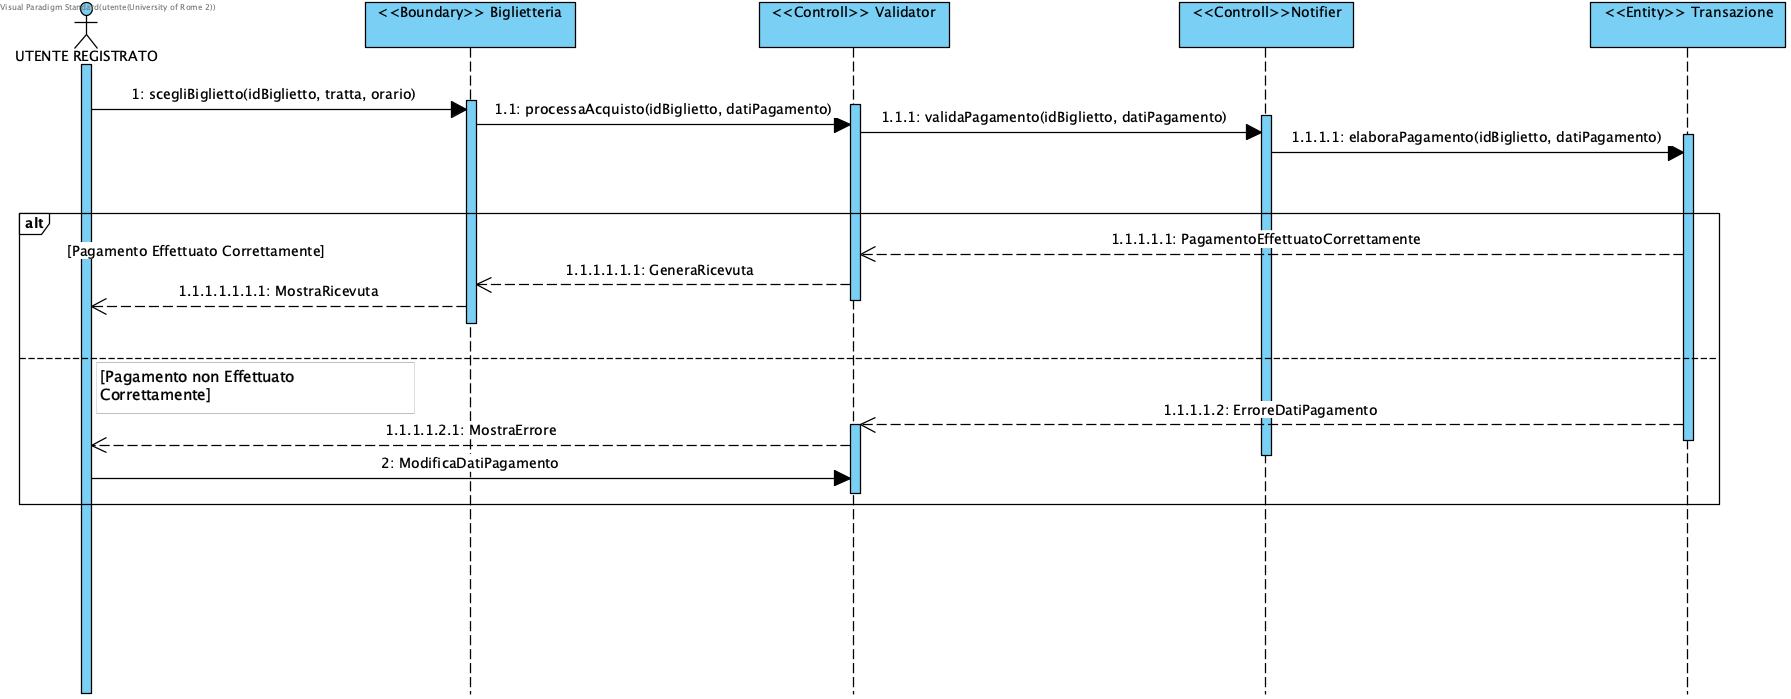
\includegraphics[width=1.0\textwidth]{Sequence Diagram/UTENTE_REGISTRATO_(Pagamento_Biglietto).png}
    \caption{}
    \label{fig:seq_ticket}
\end{figure}
\vspace{1em}
\begin{figure}[H]
    \centering
    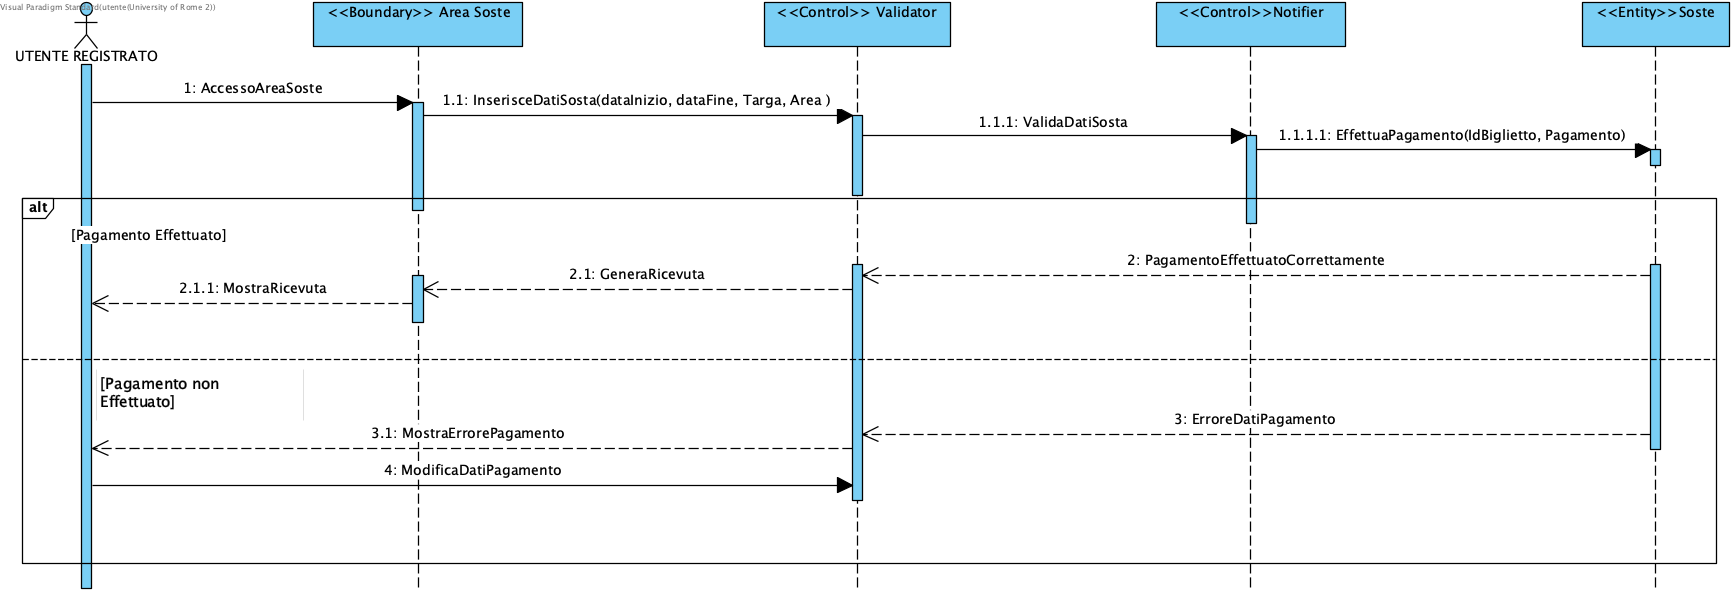
\includegraphics[width=1.0\textwidth]{Sequence Diagram/Pagamento_Soste.png}
    \caption{}
    \label{fig:seq_soste}
\end{figure}
\newpage

\noindent Oltre ai classici servizi di linea, il sistema supporta anche la prenotazione di servizi di trasporto a chiamata, noti come \textit{Demand Responsive Transport} (DRT). Come illustrato nel diagramma di Figura \ref{fig:seq_drt}, a seguito dell'inserimento dei parametri di viaggio desiderati, il sistema ricerca corse compatibili e le propone all'utente, permettendogli infine di selezionare un'opzione ed effettuare la richiesta di presa in carico.

\begin{figure}[H]
    \centering
    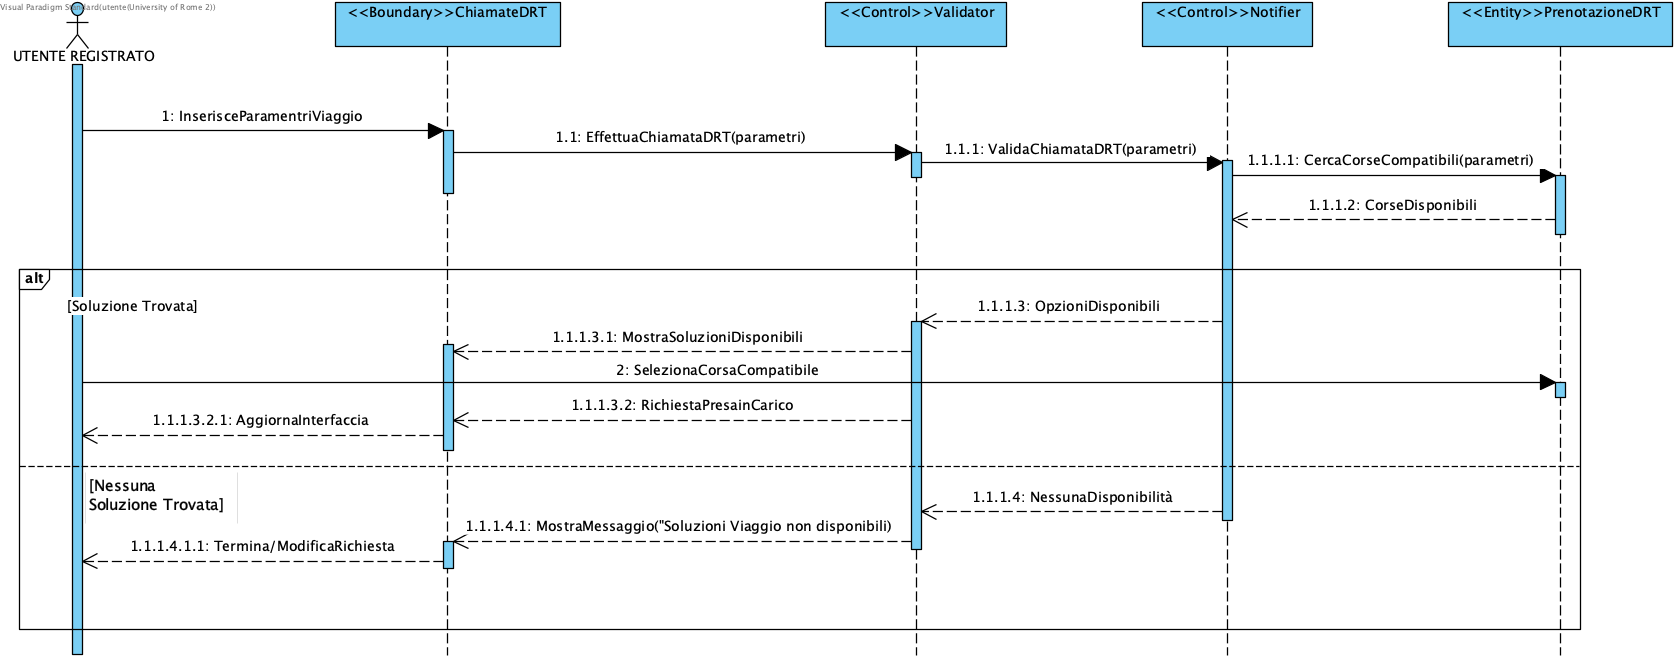
\includegraphics[width=1.0\textwidth]{Sequence Diagram/Utente_Registrato_(Prenotazione_DRT).png}
    \caption{}
    \label{fig:seq_drt}
\end{figure}

\noindent Infine, per garantire all'utente il pieno controllo sulle proprie attività passate, è prevista un'area dedicata alla consultazione dello storico. In quest'ultimo scenario (Figura \ref{fig:seq_storico}), il sistema recupera i dati delle transazioni e dei viaggi pregressi interrogando direttamente l'entità corrispondente e restituendo la lista completa a schermo, o alternativamente notificando l'assenza di dati qualora l'account non presenti attività registrate.

\begin{figure}[H]
    \centering
    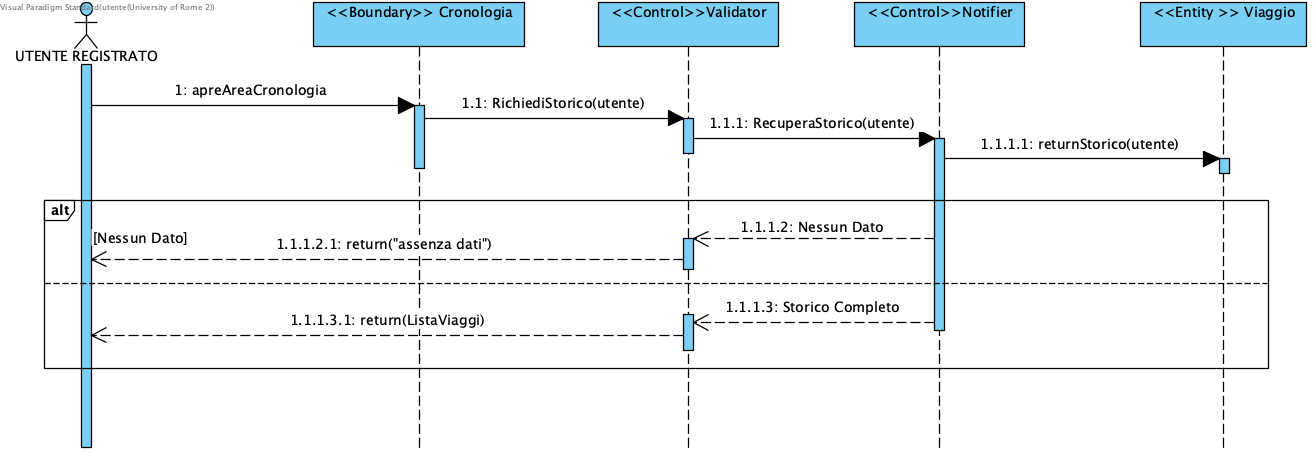
\includegraphics[width=1.0\textwidth]{Sequence Diagram/Utente_Registrato(StoricoUtente).png}
    \caption{}
    \label{fig:seq_storico}
\end{figure}
\newpage

% SEZIONE UTENTE NON REGISTRATO
\subsection*{Sequence dell'Utente non Registrato}
Passiamo ora ad analizzare le azioni che può compiere l'attore \textbf{Utente non Registrato}, cioè chi utilizza l'applicazione senza un profilo attivo. 
\\
L'operazione principale per convertire questo attore in un Utente Registrato è la procedura di registrazione. Come mostrato nella Figura \ref{fig:seq_reg}, l'utente inserisce i propri dati anagrafici nell'apposita area. Le informazioni vengono trasmesse ai moduli di controllo per la validazione: se i dati risultano incompleti o errati, il sistema richiede le opportune correzioni; in caso di dati validi, viene verificata l'unicità del Codice Fiscale interagendo con l'entità Account, per poi confermare la creazione del profilo e abilitare l'accesso ai servizi avanzati.

\begin{figure}[H]
    \centering
    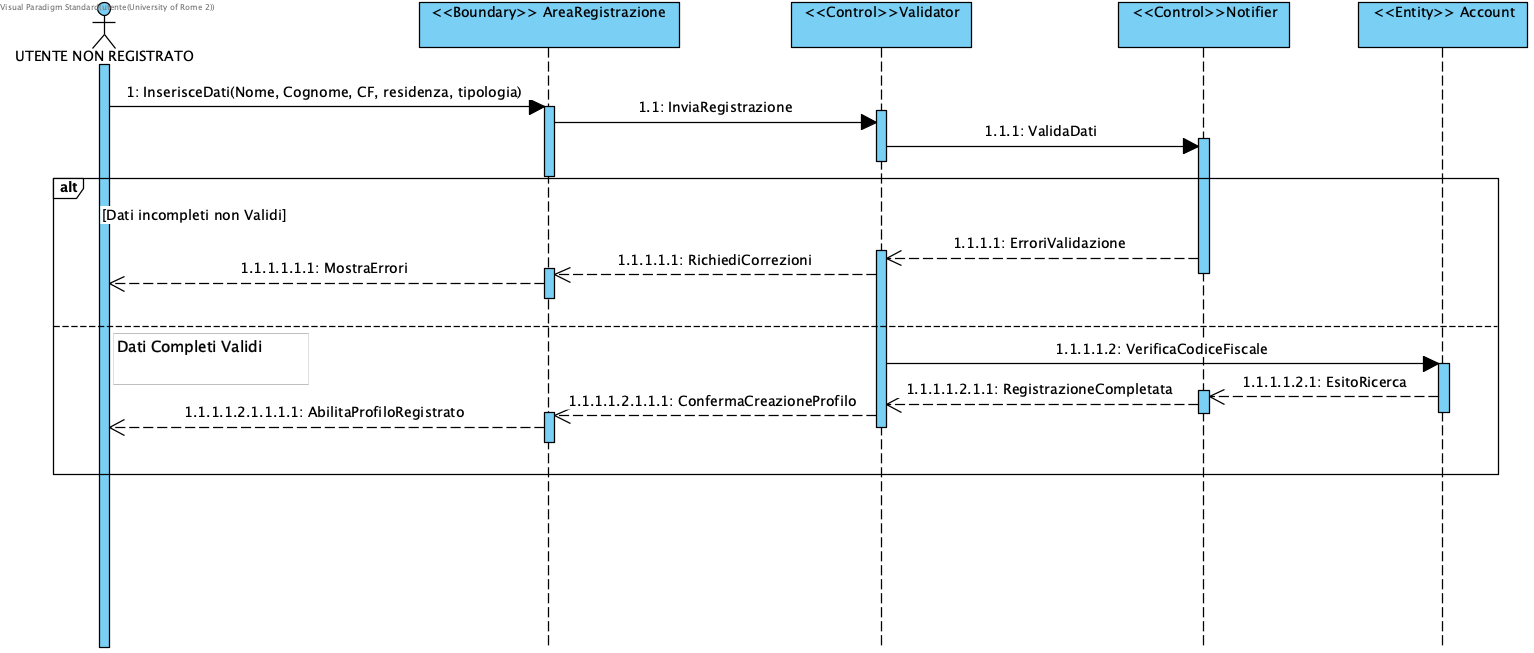
\includegraphics[width=0.8\textwidth]{Sequence Diagram/Utente_non_Registrato(Registrazione).png}
    \caption{}
    \label{fig:seq_reg}
\end{figure}
\noindent
Tuttavia, anche senza aver completato la registrazione, l'utente ha la possibilità di usufruire delle funzionalità pubbliche del sistema, come la consultazione della mobilità (Figura \ref{fig:seq_cons_unreg}). Il flusso è analogo a quello dell'utente registrato: inserendo i parametri di ricerca, il sistema convalida i dati e interroga l'entità Tratta, restituendo infine le soluzioni di viaggio, gli orari e lo stato del servizio, garantendo così un'accessibilità di base alle informazioni sul trasporto.

\begin{figure}[H]
    \centering
    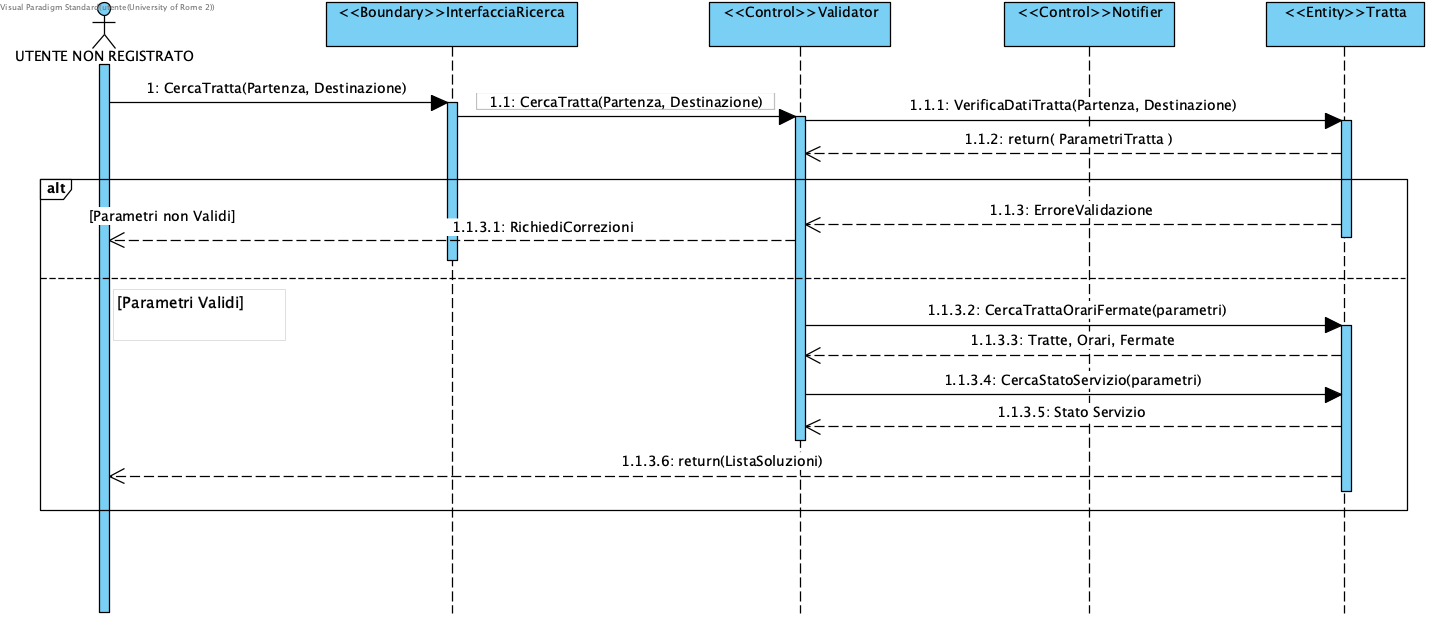
\includegraphics[width=0.8\textwidth]{Sequence Diagram/Utente_non_Registrato(Consultazione_Mobilità).png}
    \caption{}
    \label{fig:seq_cons_unreg}
\end{figure}

% SEZIONE TURISTA
\subsection*{Sequence Turista}
Un ulteriore attore principale all'interno del sistema è il \textbf{Turista}, il quale usufruisce di alcune funzionalità dedicate, pensate per agevolare l'accesso ai servizi di mobilità per periodi limitati o tramite offerte specifiche.
\\
Il primo diagramma di sequenza (Figura \ref{fig:seq_tur_cons}) illustra la procedura di consultazione dei pacchetti speciali. Il Turista accede all'area dedicata alle offerte, innescando una richiesta al sistema che, interfacciandosi con i moduli di controllo, interroga le entità preposte per recuperare le promozioni attive. A seconda dell'esito, il sistema restituisce a schermo l'elenco dei pacchetti disponibili mostrandone i dettagli, oppure notifica l'assenza di offerte attualmente valide.

\begin{figure}[H]
    \centering
    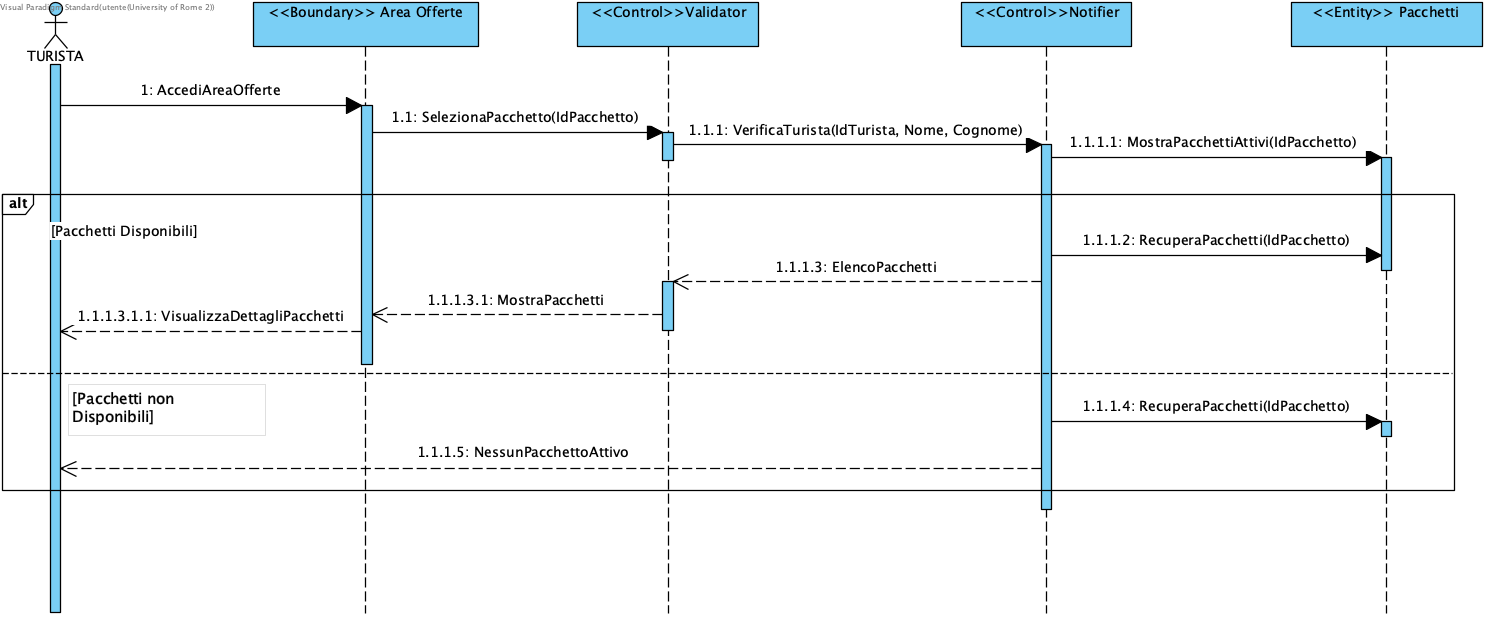
\includegraphics[width=0.8\textwidth]{Sequence Diagram/Turista_(Consultazione_Pacchetti_Speciali).png}
    \caption{}
    \label{fig:seq_tur_cons}
\end{figure}
\noindent Successivamente alla fase di consultazione, il Turista può procedere con l'acquisto di un pacchetto, come descritto nella Figura \ref{fig:seq_tur_acq}. Il diagramma mostra come, partendo dalla selezione del pacchetto desiderato e dal conseguente inserimento dei dati di pagamento, il sistema effettui le necessarie validazioni delegandole ai gestori di controllo. Se la transazione va a buon fine, il sistema genera la relativa ricevuta e conferma l'operazione aggiornando lo stato; in caso contrario, viene restituito un messaggio di errore richiedendo all'utente la modifica e il reinserimento dei dati di pagamento.
\begin{figure}[H]
    \centering
    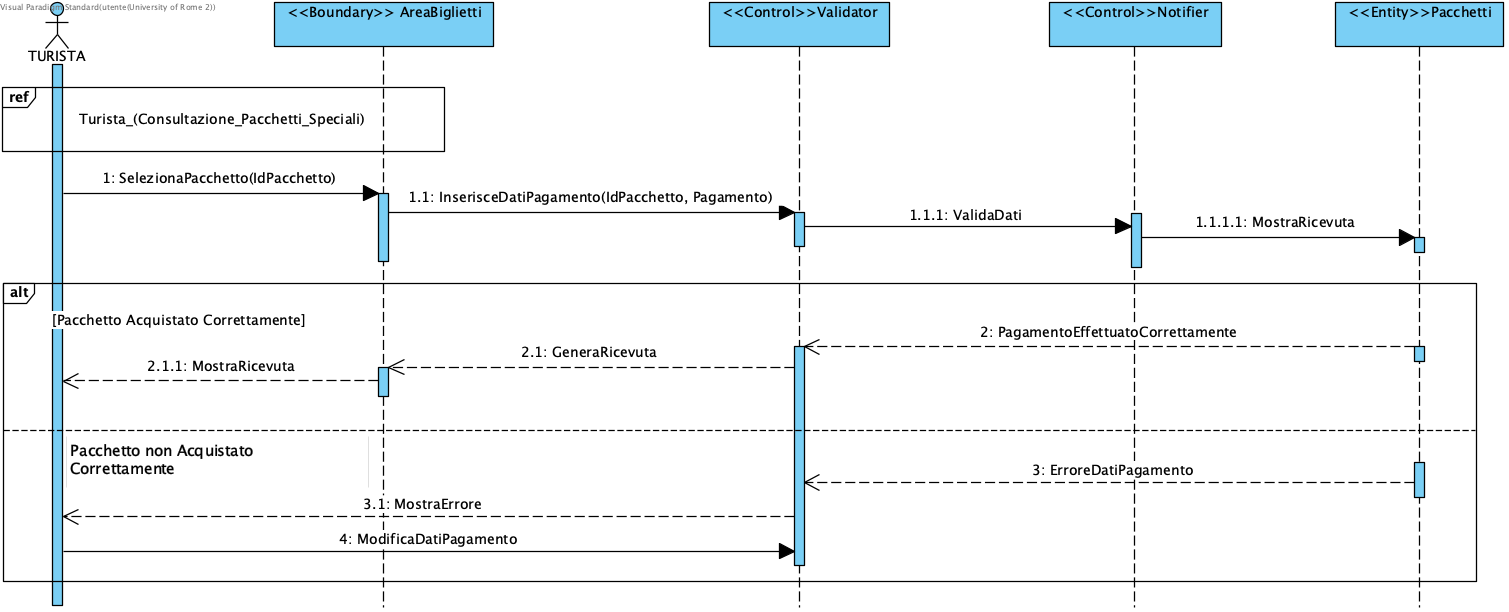
\includegraphics[width=0.8\textwidth]{Sequence Diagram/Turista_(Acquista_Pacchetto_Speciale).png}
    \caption{}
    \label{fig:seq_tur_acq}
\end{figure}


\newpage
% SEZIONE ADMIN
\subsection*{Sequence Admin}
Passiamo ora all'analisi delle operazioni riservate all'attore \textbf{Admin Ente}. 
\noindent Il primo passo fondamentale è l'accesso al sistema. Come illustrato nella Figura \ref{fig:admin_auth}, l'amministratore avvia la procedura di autenticazione. Il flusso prevede controlli decisionali per verificare il possesso di un account e la correttezza delle credenziali inserite. In caso di errore, è prevista la possibilità di recuperare la password o ritentare l'inserimento, iterando il processo fino al raggiungimento dello stato finale di accesso effettuato.
\begin{figure}[H]
    \centering
    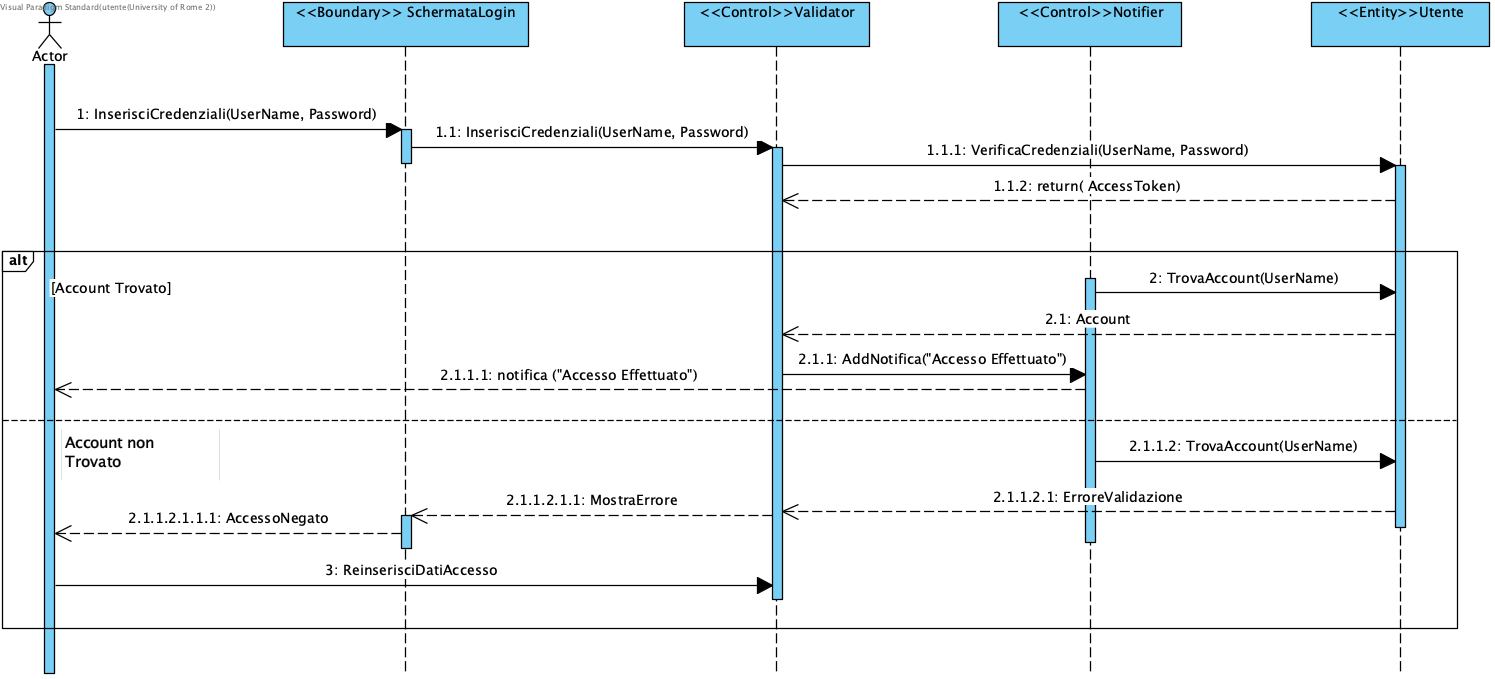
\includegraphics[width=1.0\textwidth]{Sequence Diagram/Admin_Ente_(Autenticazione_Admin).png}
    \caption{}
    \label{fig:admin_auth}
\end{figure}
\newpage
\noindent Una volta completato il login, l'Admin Ente accede all'area riservata, ovvero il Pannello di Mobilità. Il diagramma riportato in Figura \ref{fig:admin_pannello} descrive le molteplici operazioni gestionali a sua disposizione. Dal pannello principale, l'utente può diramare il flusso verso quattro sezioni specifiche: la gestione delle corse, della flotta, delle tariffe e dello staff. Dopo aver effettuato le operazioni richieste (come l'aggiunta, la modifica o la rimozione dei dati), il sistema verifica la correttezza del salvataggio, offrendo infine all'amministratore la scelta se concludere la sessione o tornare al pannello per aprire una nuova sezione.
\begin{figure}[H]
    \centering
    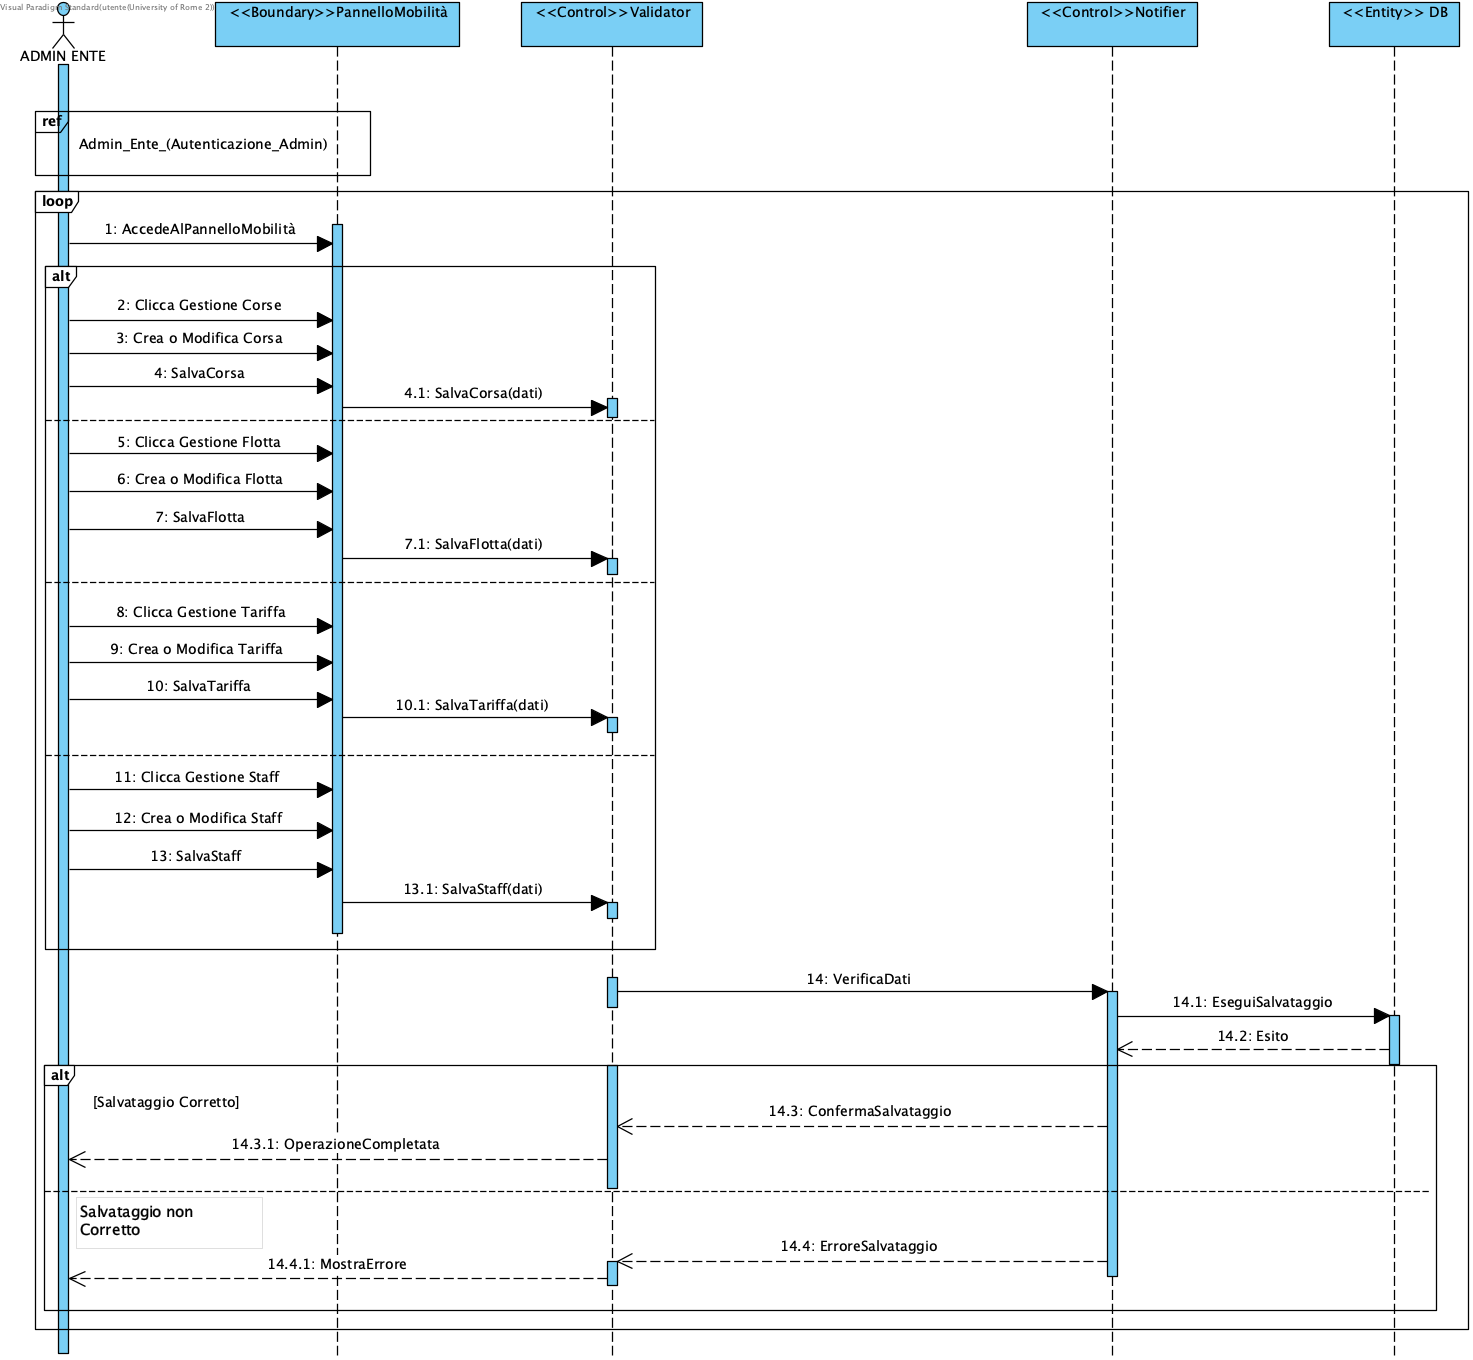
\includegraphics[width=1.0\textwidth]{Sequence Diagram/Admin_Ente_(Gestione_Pannello).png}
    \caption{}
    \label{fig:admin_pannello}
\end{figure}

\newpage
%SEQUENCE OPERAZIONE
\subsection*{Sequence Operatore}
Un ulteriore attore fondamentale per il corretto funzionamento e monitoraggio del sistema è l'\textbf{Operatore}.
\\\\ 
Il primo diagramma (Figura \ref{fig:op_auth}) descrive il processo di autenticazione, essenziale per l'accesso all'area riservata. L'operatore inserisce le proprie credenziali, le quali vengono trasmesse ai moduli di controllo per la verifica interfacciandosi con il database degli utenti. A seconda dell'esito, il sistema autorizza l'accesso generando un token di sessione, oppure notifica l'errore richiedendo un nuovo inserimento.
\begin{figure}[H]
    \centering
    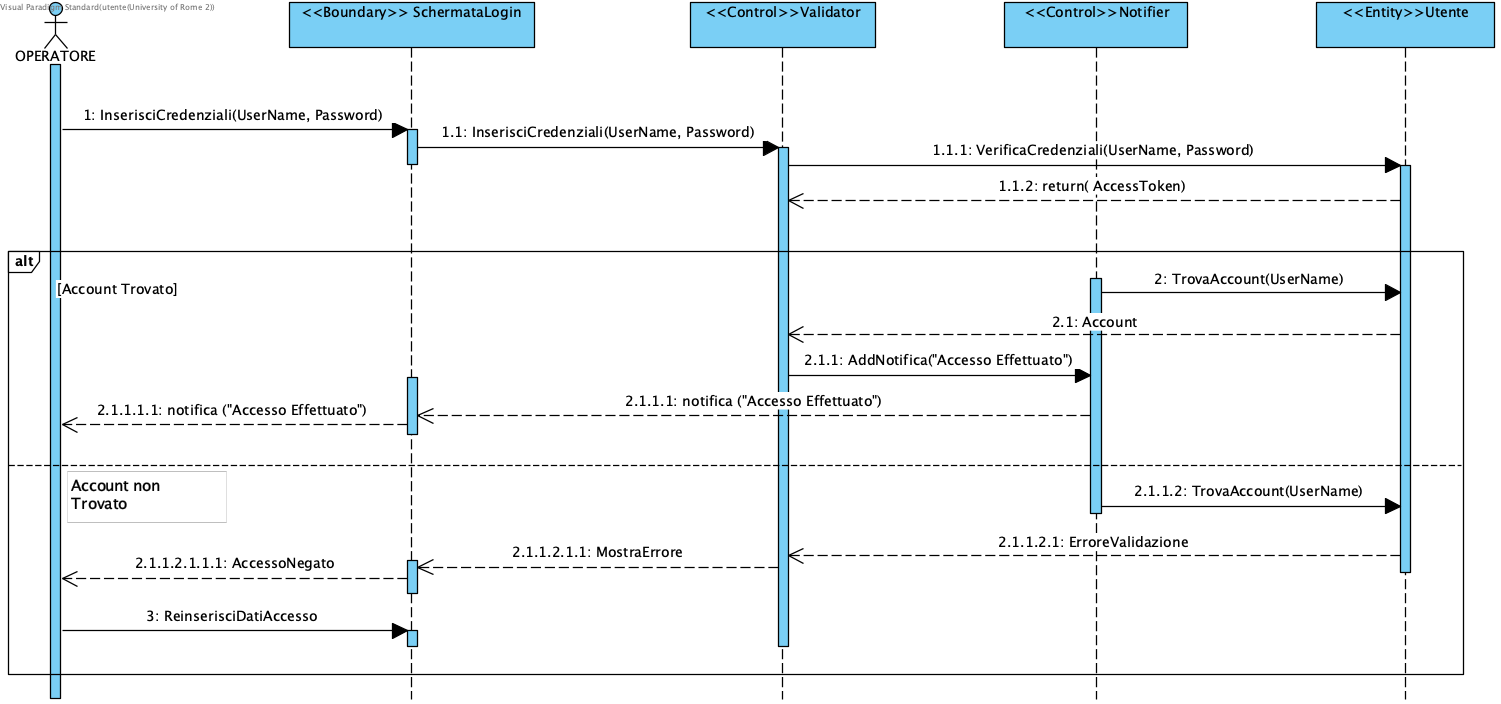
\includegraphics[width=0.8\textwidth]{Sequence Diagram/Operatore_(Autenticazione).png}
    \caption{}
    \label{fig:op_auth}
\end{figure}
\noindent Una delle mansioni principali dell'operatore è la validazione dei titoli di viaggio. Come visibile in Figura \ref{fig:op_verifica}, l'operatore può scannerizzare il QR Code del biglietto tramite il proprio pannello. Il sistema controlla la validità del formato e interroga il database per confermare l'effettiva validità del titolo. Se la scansione automatica fallisce o il formato non è valido, il sistema notifica l'errore richiedendo l'inserimento manuale dei dati.

\begin{figure}[H]
    \centering
    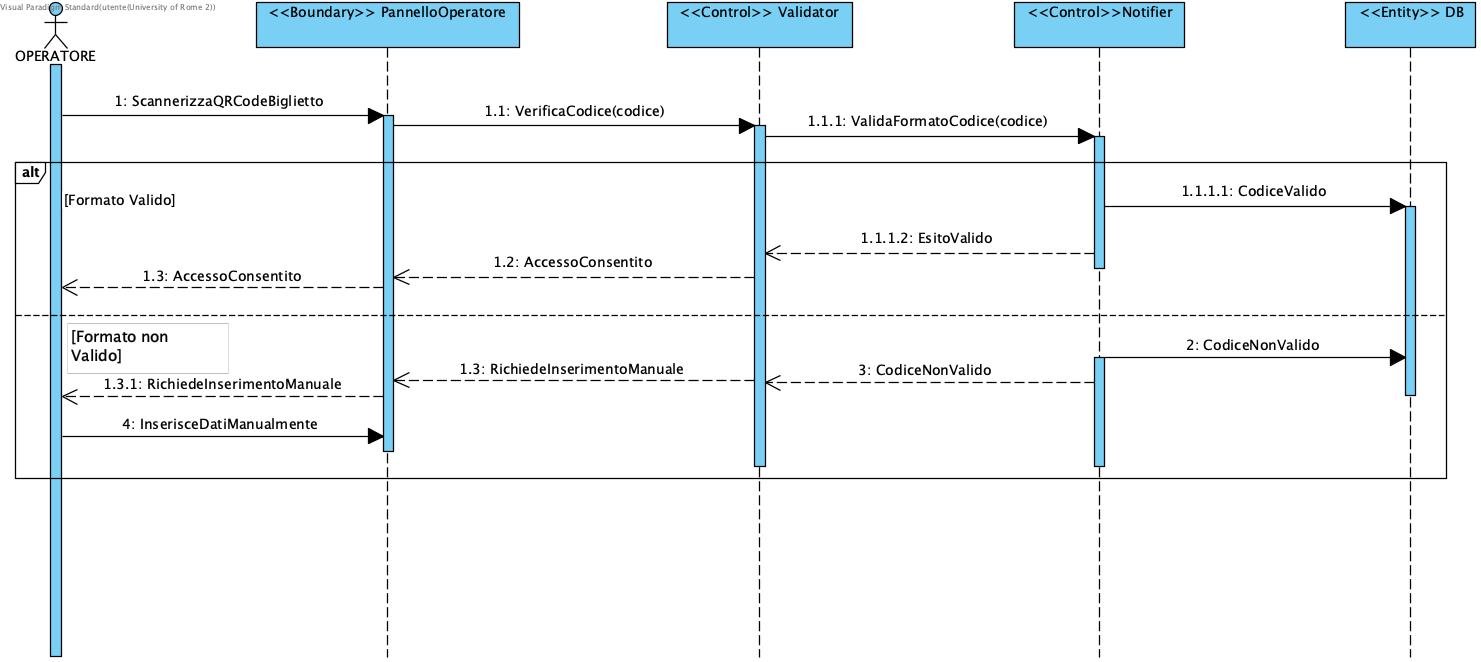
\includegraphics[width=0.8\textwidth]{Sequence Diagram/Operatore_(Verifica_Prenotazioni_e_Titoli).png}
    \caption{}
    \label{fig:op_verifica}
\end{figure}
\newpage
\noindent L'operatore è inoltre incaricato della gestione delle corse DRT (Demand Responsive Transport). Nella Figura \ref{fig:op_drt}, viene illustrato il flusso di presa in carico delle richieste: l'operatore visualizza a schermo le prenotazioni e comunica al sistema la propria decisione (accettazione o rifiuto). I controllori validano i parametri inseriti e aggiornano lo stato della prenotazione all'interno del database.
\begin{figure}[H]
    \centering
    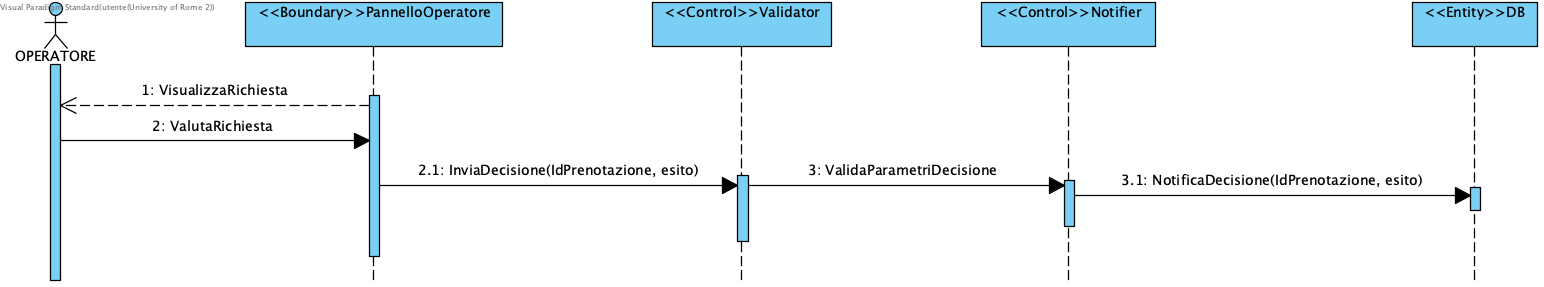
\includegraphics[width=1.0\textwidth]{Sequence Diagram/Operatore_(Gestione_Corse_DRT).png}
    \caption{}
    \label{fig:op_drt}
\end{figure}
\noindent Infine, è prevista la funzionalità di aggiornamento dello stato del servizio, utile per comunicare in tempo reale eventuali ritardi o variazioni. Nel diagramma di Figura \ref{fig:op_stato}, l'operatore seleziona il mezzo e i parametri della corsa per inviare l'aggiornamento. Il backend elabora la richiesta e tenta il salvataggio sul database; l'operazione si conclude con la notifica di successo a schermo o, in caso di anomalie, con un messaggio di errore che invita a ripetere l'inserimento.
\begin{figure}[H]
    \centering
    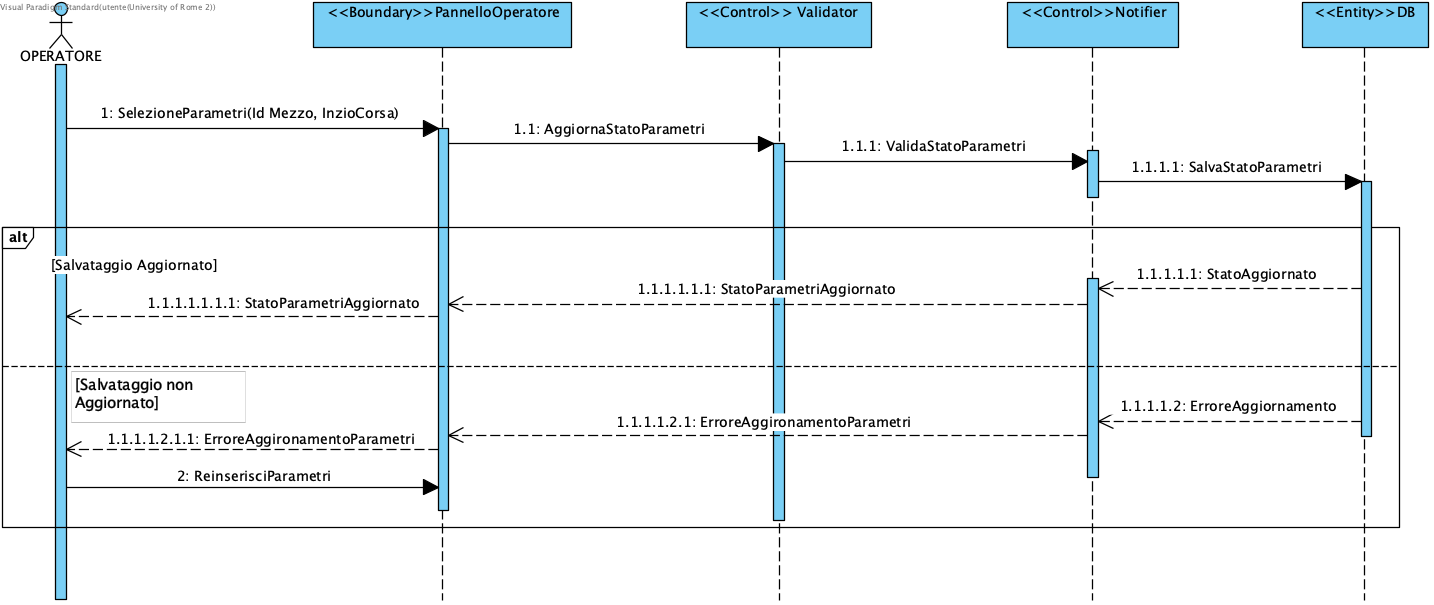
\includegraphics[width=1.0\textwidth]{Sequence Diagram/Operatore_(Stato_Servizio).png}
    \caption{}
    \label{fig:op_stato}
\end{figure}

\newpage
% SEQUENCE FUNZIONARIO COMUNALE
\subsection*{Sequence Funzionario Comunale}
Un altro attore di sistema che andiamo ad analizzare è il \textbf{Funzionario Comunale}. Questa figura istituzionale ha il compito di gestire la viabilità cittadina, inserendo ordinanze e percorsi alternativi che avranno un impatto diretto sui servizi di mobilità.
\\\\
Analogamente agli altri attori, il primo passo per operare all'interno del sistema è l'autenticazione. Come mostrato nella Figura \ref{fig:fc_auth}, il funzionario inserisce le proprie credenziali nella schermata di login. I dati vengono processati dai moduli di controllo per verificarne la validità interrogando il database. In caso di esito positivo, viene garantito l'accesso; in caso contrario, il sistema respinge la richiesta notificando l'errore e invitando a ripetere l'operazione.
\begin{figure}[H]
    \centering
    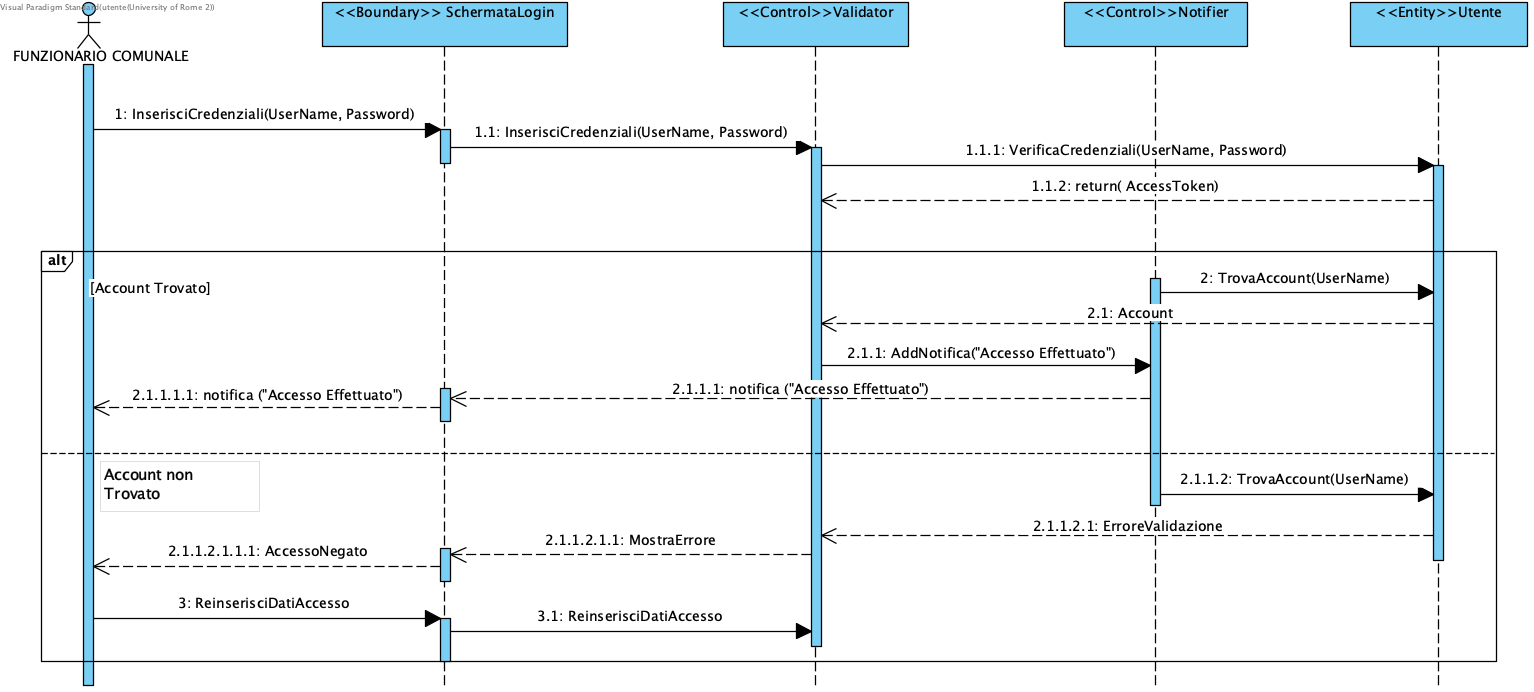
\includegraphics[width=0.9\textwidth]{Sequence Diagram/Funzionario_Comunale_(Autenticazione).png}
    \caption{}
    \label{fig:fc_auth}
\end{figure}
\noindent Una delle funzionalità centrali per questo attore è la gestione delle ordinanze (Figura \ref{fig:fc_ordinanze}). Il funzionario carica il documento ufficiale e seleziona le aree coinvolte tramite l'apposita sezione. Il sistema valida il formato del documento: se non risulta conforme, l'operazione viene interrotta con una richiesta di correzione; se valido, l'ordinanza viene salvata nel database e il sistema restituisce un messaggio di conferma, rendendo l'avviso visibile.
\begin{figure}[H]
    \centering
    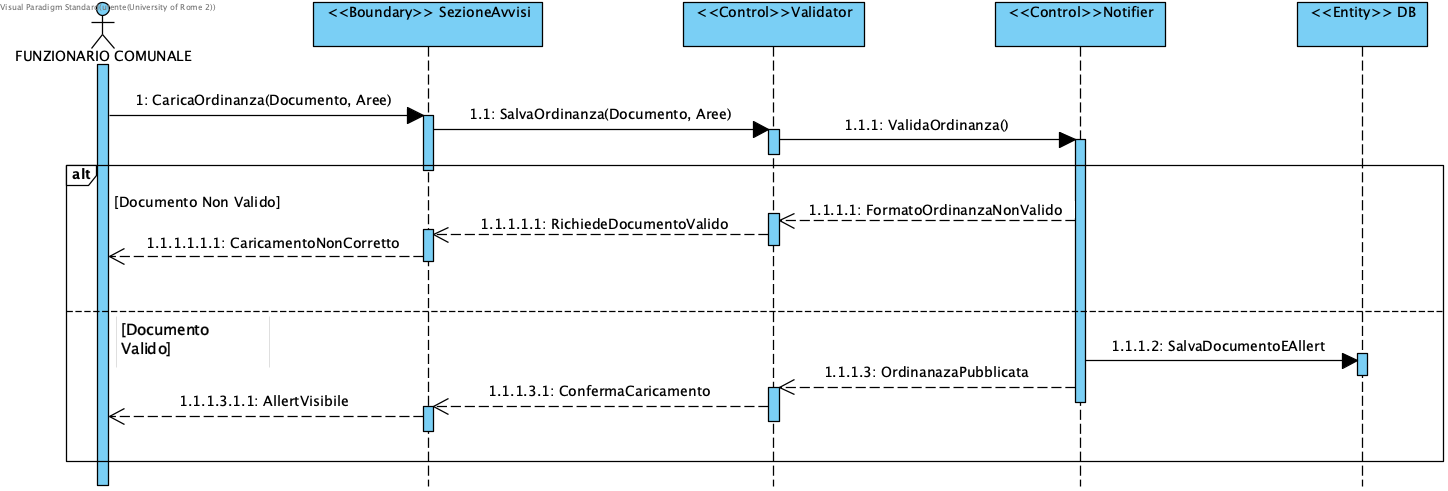
\includegraphics[width=0.9\textwidth]{Sequence Diagram/Funzionario_Comunale_(Gestione_Ordinanze).png}
    \caption{}
    \label{fig:fc_ordinanze}
\end{figure}
\newpage
\noindent A seguito di un'ordinanza, può rendersi necessario modificare la viabilità. Il diagramma di Figura \ref{fig:fc_percorsi} illustra l'inserimento di un percorso alternativo. Richiamando le informazioni dell'ordinanza appena gestita, il funzionario traccia la deviazione; il sistema, dopo aver validato il tracciato, provvede a generare e salvare il nuovo percorso all'interno della base di dati.
\begin{figure}[H]
    \centering
    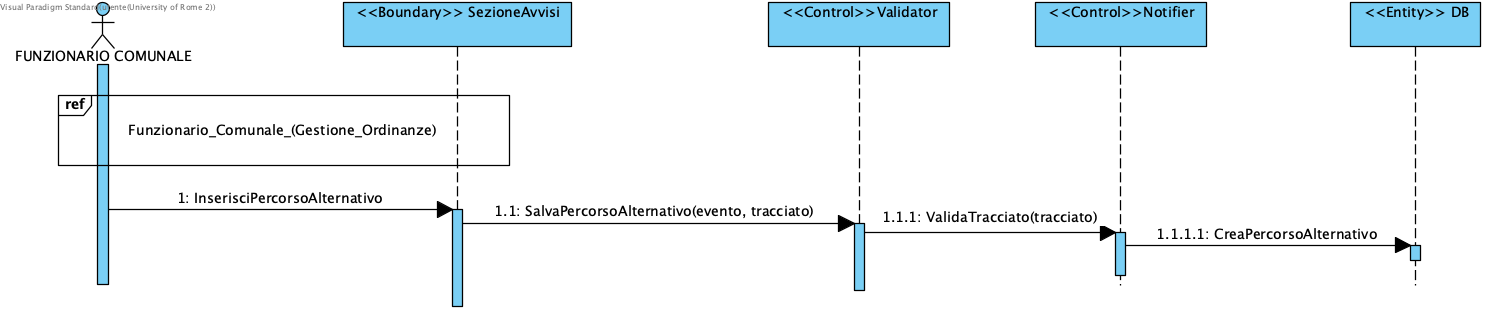
\includegraphics[width=1.0\textwidth]{Sequence Diagram/Funzionario_Comunale_(Gestione_Percorsi).png}
    \caption{}
    \label{fig:fc_percorsi}
\end{figure}
\noindent Infine, per garantire un coordinamento efficace, il funzionario deve poter comunicare le variazioni agli enti terzi. Come visibile nella Figura \ref{fig:fc_notifiche}, l'attore manda un messaggio specificando i destinatari e la relativa ordinanza. I controllori validano il testo e i destinatari, per poi procedere con l'inoltro effettivo. Il sistema conferma al funzionario l'avvenuto invio o segnala un'eventuale mancata ricezione in caso di anomalia.
\begin{figure}[H]
    \centering
    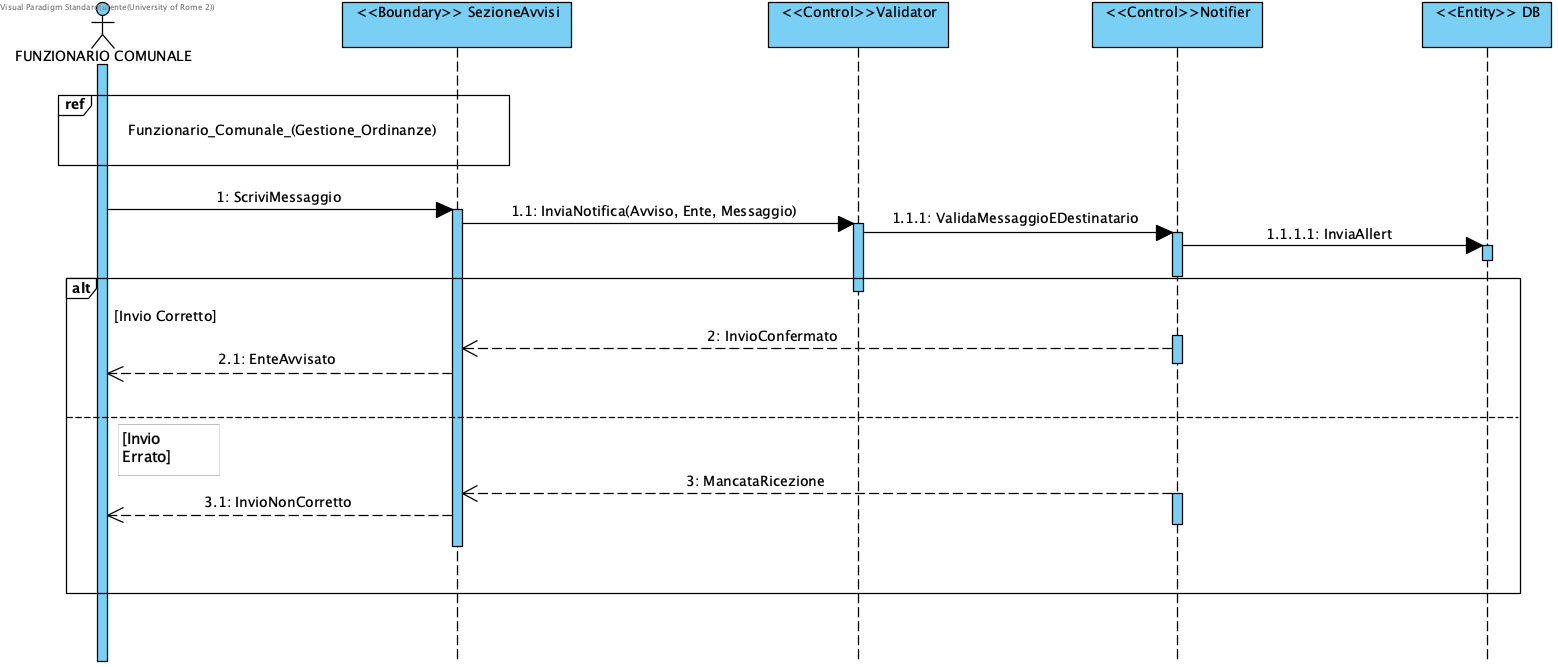
\includegraphics[width=1.0\textwidth]{Sequence Diagram/Funzionario_Comunale_(Notifiche_Enti).png}
    \caption{}
    \label{fig:fc_notifiche}
\end{figure}

\newpage
% SEQUENCE PAYMENT
\subsection*{Sequence Payment}
Infine, ma non per importanza, ci occupiamo della gestione delle transazioni finanziarie, attraverso l'attore \textbf{Payment}. I diagrammi di sequenza seguenti illustrano l'interazione tra l'utente (tramite l'applicazione front-end), il backend MaaS, i gateway di pagamento esterni e il database. 
\\\\
Il processo di elaborazione dei pagamenti (Figura \ref{fig:seq_pagamenti}) si attiva quando l'utente inserisce i propri dati per l'acquisto di un servizio. L'App Front-End inoltra tali informazioni al Back-End MaaS, il quale si fa carico di orchestrare la transazione comunicando in modo sicuro con il Gateway Esterno. In caso di esito positivo, il sistema registra la transazione nel database e restituisce all'utente la ricevuta di pagamento. Qualora i dati risultino non validi o la transazione venga rifiutata, viene registrato il fallimento e notificata a schermo la mancata validazione.
\begin{figure}[H]
    \centering
    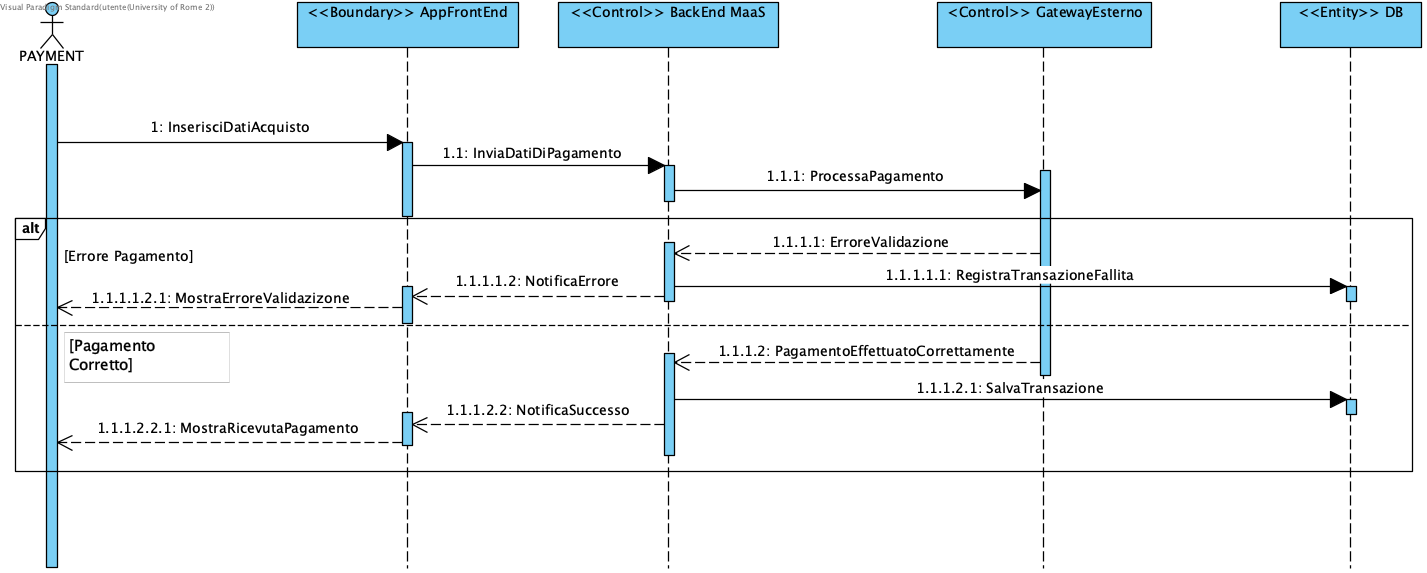
\includegraphics[width=0.9\textwidth]{Sequence Diagram/Payment_(Elaborazioni_Pagamenti).png}
    \caption{}
    \label{fig:seq_pagamenti}
\end{figure}
\noindent
Per quanto riguarda la gestione dei rimborsi, illustrata nella Figura \ref{fig:seq_rimborsi}, prevede una richiesta di rimborso iniziale da parte dell'utente. Successivamente il Back-End MaaS esegue un controllo preliminare interrogando il Database per verificare che la transazione rispetti i termini temporali e le condizioni di rimborsabilità. Se i termini risultano scaduti o non validi, la procedura viene bloccata mostrando un messaggio di negazione. Se i controlli hanno esito positivo, il Back-End inoltra la richiesta al Gateway Esterno per l'erogazione effettiva, concludendo il flusso con l'aggiornamento dello stato nel Database e la visualizzazione della notifica di successo.
\begin{figure}[H]
    \centering
    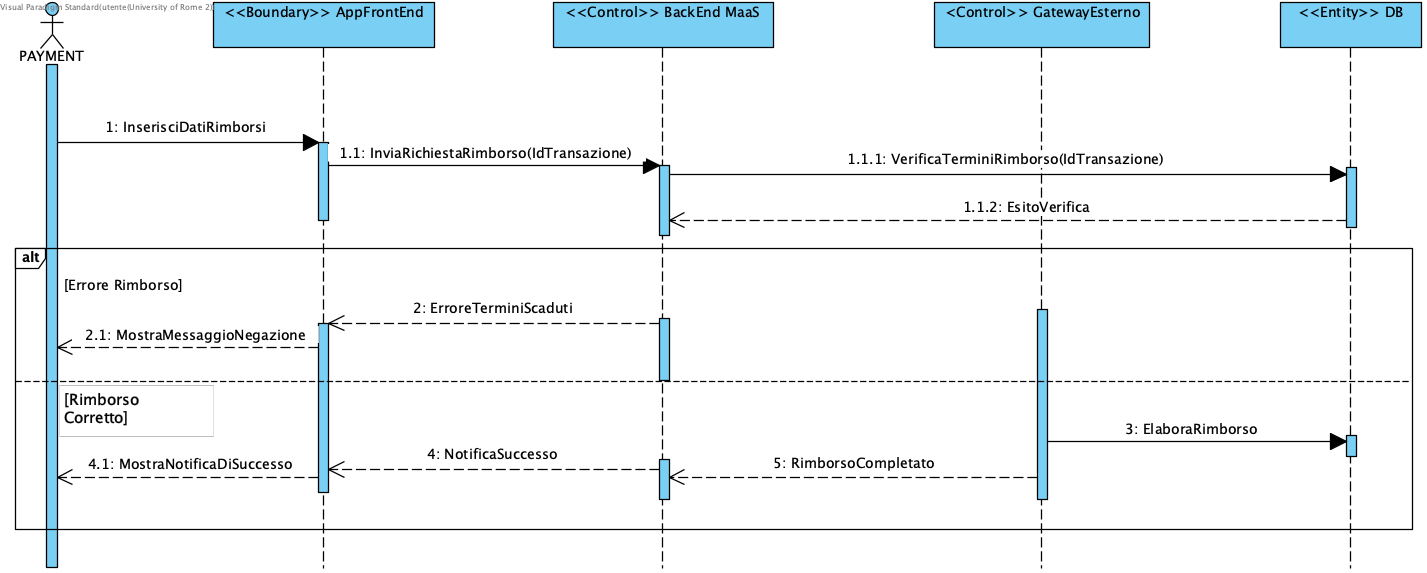
\includegraphics[width=0.9\textwidth]{Sequence Diagram/Payment_(Elaborazione_Rimborsi).png}
    \caption{}
    \label{fig:seq_rimborsi}
\end{figure}


\newpage

\chapter{Implementazione}
Sulla base dell'analisi dei requisiti e delle scelte progettuali illustrate nei capitoli precedenti, il presente capitolo approfondisce la realizzazione tecnica della piattaforma \emph{Mobility as a Service} (MaaS) sviluppata per il contesto territoriale di Scicli. L'obiettivo è descrivere in maniera sistematica l'architettura software, l'implementazione tecnica del sistema, descrivendo l'architettura generale, le tecnologie impiegate e le logiche di sviluppo adottate per la sua costruzione.
\\
L'implementazione è stata orientata alla costruzione di un prototipo integrato, in grado di offrire un'interfaccia di accesso differenziata in base alla tipologia di utente. 
\\
Per ridurre i tempi di sviluppo e la complessità delle attività infrastrutturali, il progetto adotta un approccio basato su servizi \emph{Backend-as-a-Service} (BaaS), integrato con un backend applicativo dedicato. 
\\
È opportuno precisare fin da subito che non tutte le richieste del frontend transitano attraverso il backend Java. L'esame del codice mostra un'integrazione \emph{ibrida}: alcune operazioni utilizzano le API REST del server, mentre altre interrogano direttamente Cloud Firestore.

\section{Architettura generale della piattaforma: approccio BaaS e separazione delle responsabilità}

Con l'espressione \emph{Backend-as-a-Service} si indica un modello di sviluppo nel quale alcune capacità tipiche del livello server sono offerte come servizi gestiti da un fornitore esterno. In questo modello l'applicazione non deve necessariamente predisporre e amministrare autonomamente ogni componente relativo all'autenticazione, alla memorizzazione dei dati, alla disponibilità dei servizi o alle operazioni di manutenzione infrastrutturale. Lo sviluppatore può quindi concentrare una parte maggiore dell'attività sulle funzionalità specifiche del dominio applicativo. L'adozione di un BaaS non elimina, tuttavia, la necessità di progettare con attenzione il modello dei dati, la sicurezza degli accessi e le regole applicative; tali responsabilità rimangono in capo a chi sviluppa il sistema.
\\
Nel caso di MaaS Scicli, la soluzione individuata combina due approcci complementari. 
\begin{itemize}
    \item Firebase costituisce l'infrastruttura gestita per l'identità
    \item mentre Spring Boot svolge il ruolo di backend personalizzato per quelle operazioni che richiedono una mediazione applicativa.
\end{itemize}
La Figura~\ref{fig:architettura} rappresenta l'articolazione dei principali componenti. Le interazioni tra frontend e backend avvengono mediante chiamate HTTP che utilizzano risorse identificate da URI e, prevalentemente, messaggi in formato JSON. 
Il backend, attraverso Firebase Admin SDK, accede ai dati e verifica i token di autenticazione. Parallelamente, il frontend utilizza il Firebase JavaScript SDK per avviare sessioni di autenticazione, eseguire alcune letture dirette e ricevere notifiche di aggiornamento sui documenti Firestore.

\begin{figure}[htbp]
\centering
\begin{tikzpicture}[
  font=\small,
  box/.style={
    draw=black!65,
    rounded corners=3pt,
    align=center,
    minimum height=1.15cm,
    text width=4.5cm,
    fill=gray!6
  },
  smallbox/.style={
    draw=black!65,
    rounded corners=3pt,
    align=center,
    minimum height=1.15cm,
    text width=3.5cm,
    fill=gray!3
  },
  arrow/.style={-{Latex[length=2mm]}, line width=.75pt},
  both/.style={{Latex[length=2mm]}-{Latex[length=2mm]}, line width=.75pt}
]

% Nodi principali
\node[box] (client) at (0,3.5)
{\textbf{Browser / PWA}\\ React Native Web\\ Vite e React Router};

\node[box] (server) at (8,3.5)
{\textbf{Spring Boot}\\ Interfaccia compilata\\ API e controlli applicativi};

% Nodi secondari
\node[smallbox] (auth) at (0,0)
{\textbf{Firebase Authentication}\\ Identità e token};

\node[smallbox] (firestore) at (5,0)
{\textbf{Cloud Firestore}\\ Dati applicativi};

\node[smallbox] (h2) at (10,0)
{\textbf{H2 in memoria}\\ Modulo GTFS};

% Collegamenti
\draw[both] (client.east) -- node[above, align=center, font=\scriptsize]
{HTTP/JSON\\token ove richiesto} (server.west);

\draw[both] (client.south) -- node[left, align=center, font=\scriptsize]
{SDK client\\autenticazione} (auth.north);

% Spring Boot -> Cloud Firestore
\draw[arrow]
    ([xshift=-1.1cm]server.south)
    -- node[left, font=\scriptsize, xshift=-2pt]
       {Admin SDK}
       ++(0,-1.1cm)
    -| (firestore.north);

% Spring Boot -> H2
\draw[arrow]
    ([xshift=1.1cm]server.south)
    -- node[right, font=\scriptsize, xshift=2pt]
       {JPA / repository}
       ++(0,-1.4cm)
    -| (h2.north);
    
\end{tikzpicture}
\caption{Architettura generale del sistema.}
\label{fig:architettura}
\end{figure}
\section{React Native per lo sviluppo Front-end}

Per il frontend è stato adottato \emph{React Native}, framework che consente di realizzare interfacce applicative utilizzando il modello a componenti di React. L'impiego di componenti riutilizzabili permette di separare le parti visive dalle procedure di caricamento e trattamento dei dati, favorendo un'organizzazione modulare dell'applicazione. 
\\ 
In questa fase prototipale, l'applicazione non prevede la distribuzione tramite gli store digitali (come Google Play Store o Apple App Store), né la generazione di pacchetti nativi dedicati (APK o IPA). Il sistema è invece fruibile come Progressive Web App (PWA) integrata direttamente nel server backend Spring Boot, il quale si occupa di distribuire contestualmente sia l'interfaccia frontend compilata sia le API REST sullo stesso indirizzo di rete. Di conseguenza, il dispositivo mobile dell'utente non esegue il codice di backend, ma vi accede semplicemente tramite browser. L'installazione dell'applicativo sul telefono è gestita direttamente dal browser web (ad esempio, mediante l'opzione \textit{"Aggiungi a schermata Home"}), garantendo un'esperienza d'uso a schermo intero affine a quella di un'applicazione nativa. È opportuno precisare che, affinché le funzionalità PWA e i servizi hardware del dispositivo (come la geolocalizzazione) operino correttamente su un telefono fisico, la distribuzione del sistema richiede un contesto di rete sicuro, tipicamente implementato tramite protocollo HTTPS.
\begin{figure}[H]
    \centering
    
\includegraphics[width=0.3\linewidth]{Foto/IMG_5841-removebg-preview.png}
    \caption{}
    \label{fig:placeholder}
\end{figure}
\noindent
L'uso di React Native si presta inoltre alla realizzazione di un'interfaccia multipiattaforma, mantenendo una base di codice largamente condivisa.
\\
Al termine della fase di collaudo, si procederà al rilascio finale compilando il codice sorgente nei pacchetti nativi dell'applicazione. In questo modo, l'utente finale non dovrà avviare alcun server locale da terminale o interagire con strumenti di sviluppo, ma potrà scaricare e installare l'applicazione in modo semplice, trasparente e sicuro direttamente dagli store digitali ufficiali, come Google Play Store e Apple App Store.
\\
La \texttt{HomeScreen.js} rappresenta l'hub centrale per l'utente. Da questa interfaccia, dotata di una barra di navigazione personalizzata e di un layout scorrevole, l'utente può cercare rapidamente un luogo o un servizio. Questa schermata integra collegamenti rapidi per l'acquisto di biglietti per la sosta e fornisce una serie di pulsanti per instradare le diverse tipologie di utenti (Cittadino, Turista, Admin Ente, Operatore, Funzionario) verso le rispettive dashboard dedicate.
\\
L'applicazione prevede una vista iniziale comune, seguita da percorsi differenziati in funzione del profilo restituito dopo l'accesso. Il frontend riconosce i ruoli \texttt{CITTADINO}, \texttt{TURISTA}, \texttt{OPERATORE}, \texttt{FUNZIONARIO}, \texttt{ADMIN} e \texttt{ADMIN\_ENTE}.
\\
Sono presenti, tra le altre, le schermate \texttt{ConsultazioneMobilita}, \texttt{PrenotazioneDRT}, \texttt{PaymentSosta}, \texttt{PaymentBiglietti}, \texttt{AcquistoSpeciali}, \texttt{GestioneFlotta}, 
\\\texttt{GestioneStaff}, \texttt{GestioneCorse} e \texttt{GestioneOrdinanze} e le altre operazioni che i vari utenti effettuano, elencate nei vari activity diagram. 
\\
Per gli utenti non istituzionali, il codice di login opera inoltre una distinzione tra cittadino e turista sulla base del comune di residenza presente nel profilo, attribuendo la categoria \texttt{CITTADINO} al valore ``Scicli'' e \texttt{TURISTA} negli altri casi. Si tratta di una regola di navigazione implementata nel client, distinta dall'attribuzione formale dei permessi lato server.
\\
Di seguito, è descritta una tabella contenente i profili, i rispettivi nomi dove sono implementati quest'ultimi.

\begin{table}[H]
\centering
\small
\begin{tabular}{P{3.0cm}P{5.0cm}P{6cm}}
\toprule
\textbf{Profilo} & \textbf{Vista di riferimento} & \textbf{Funzioni presentate nel prototipo}\\
\midrule
Cittadino & \texttt{CittadinoDashboard} & Consultazione della mobilità, sosta, richieste DRT e accesso a pagine informative.\\
Turista & \texttt{TuristaDashboard} & Accesso a servizi di mobilità e soluzioni rivolte ai visitatori, inclusi pacchetti dimostrativi.\\
Operatore & \texttt{OperatoreDashboard} & Gestione delle richieste di corsa e visualizzazione delle comunicazioni.\\
Funzionario & \texttt{FunzionarioDashboard} & Consultazione e gestione di informazioni amministrative; alcune operazioni sono ancora locali alla schermata.\\
Amministratore dell'ente & \texttt{AdminEnteDashboard} & Gestione della flotta, del personale, delle corse e delle tariffe.\\
\bottomrule
\end{tabular}
\caption{}
\label{tab:ruoli}
\end{table}

\noindent
Nel frontend sono presenti due modalità di recupero delle informazioni. 
\begin{itemize}
    \item La prima utilizza \texttt{fetch}, funzione per l'invio di richieste HTTP agli endpoint Spring Boot.
    \item La seconda utilizza funzioni dello SDK Firestore.
\end{itemize}
\vspace{0.5em}
Questa combinazione di chiamate REST e comunicazioni dirette con il database rende il prototipo flessibile, ma introduce due modelli di accesso ai dati che devono rimanere coerenti. In prospettiva è opportuno stabilire criteri architetturali espliciti: riservare al backend le operazioni che contengono regole di business, vincoli economici o autorizzazioni complesse e consentire accessi diretti solo quando siano necessari e adeguatamente controllati dalle regole di sicurezza Firestore.

\section{Implementazione del backend e delle API REST}
Il backend è implementato in Java e utilizza Spring Boot, framework che semplifica la configurazione e l'organizzazione di applicazioni server. 
\\
In particolare, la classe \texttt{FirebaseService} centralizza numerose operazioni verso Firestore: lettura delle informazioni sul trasporto, gestione dei profili, registrazione di prenotazioni e transazioni, trattamento delle ordinanze e funzioni di amministrazione. Sebbene tale concentrazione sia pratica nelle prime fasi prototipali, in un'evoluzione del sistema sarebbe preferibile separare il servizio in componenti specializzati per dominio funzionale, allo scopo di migliorare coesione, manutenibilità e testabilità.
\\
Il backend è organizzato intorno a controller contrassegnati dall'annotazione: 
\\
\texttt{@RestController}, che rendono accessibili le funzionalità applicative tramite endpoint. L'annotazione \texttt{@RequestMapping} individua il percorso comune della risorsa, mentre annotazioni quali \texttt{@GetMapping}, \texttt{@PostMapping}, \texttt{@PutMapping} e \texttt{@DeleteMapping} specificano le operazioni consentite. 
\\
I controller restituiscono frequentemente oggetti \texttt{ResponseEntity}, mediante i quali è possibile associare alla risposta un codice HTTP e un contenuto JSON.

\begin{longtable}{P{4.0cm}P{5.3cm}P{5.0cm}}
\label{tab:api}\\
\toprule
\textbf{Controller} & \textbf{Percorso principale} & \textbf{Responsabilità}\\
\midrule
\endfirsthead

\toprule
\textbf{Controller} & \textbf{Percorso principale} & \textbf{Responsabilità}\\
\midrule
\endhead

\texttt{Autenticazione} &
\texttt{/api/auth/login} e \texttt{/api/auth/register} &
Validazione del token e lettura o registrazione del profilo.\\

\texttt{Consultazione}\newline\texttt{Controller} &
\texttt{/api/linee/cerca} e \texttt{/api/linee/}\newline\texttt{cercaVia} &
Ricerca di linee e fermate.\\

\texttt{PannelloDRT} &
\texttt{/api/drt/prenota} &
Inserimento delle richieste di trasporto a chiamata.\\

\texttt{OrdinanzeController} &
\texttt{/api/ordinanze} &
Lettura e pubblicazione delle ordinanze.\\

\texttt{PannelloGestione}\newline\texttt{Admin} &
\texttt{/api/admin/bus} e \texttt{/api/admin/staff} &
Gestione di flotta e personale.\\

\texttt{DemoWallet}\newline\texttt{Controller} &
\texttt{/api/demo-wallet/}\newline\texttt{payments} &
Creazione, consultazione e variazione dello stato delle operazioni simulate.\\

\texttt{PercorsoGtfs}\newline\texttt{Controller} &
\texttt{/api/cerca-}\newline\texttt{percorso} &
Interrogazione di percorsi diretti secondo il modello GTFS.\\

\bottomrule
\caption{}
\end{longtable}
\noindent
Il componente \texttt{FirebaseService} svolge il ruolo di intermediario verso Firebase. Attraverso il suo impiego, i controller possono delegare la lettura e la modifica dei documenti senza duplicare in ogni metodo la configurazione dei client o le istruzioni di accesso a Firestore. Il modulo GTFS segue una separazione più articolata, composta da \texttt{PercorsoGtfsController}, \texttt{PercorsoGtfsService} e \texttt{PercorsoGtfsRepository}: il controller riceve i parametri, il servizio coordina la ricerca e il repository esegue le query sul database relazionale.
\\
Una parte significativa della robustezza del sistema dipende dalla validazione dei valori forniti dall'utente. Nel controller di autenticazione la registrazione richiede campi testuali non vuoti e ne controlla la lunghezza; il controller delle ordinanze applica vincoli al titolo, al testo e alla data; il modulo dei pagamenti verifica il tipo di operazione, la struttura dei parametri e gli intervalli ammessi. In caso di richiesta non valida, i metodi possono restituire \texttt{400 Bad Request}; nel caso di credenziali mancanti o non valide, il modulo di login restituisce \texttt{401 Unauthorized}. Sono inoltre presenti casi di \texttt{403 Forbidden}, \texttt{404 Not Found}, \texttt{409 Conflict} e \texttt{500 Internal Server Error}.

\section{Modello dei dati e integrazione con Cloud Firestore}

Cloud Firestore adotta un modello NoSQL basato su collezioni e documenti. Ciascun documento è identificato da una chiave e contiene un insieme di campi, che possono rappresentare valori testuali, numerici, temporali, booleani o strutture composite, come array e mappe. A differenza di un database relazionale tradizionale, la struttura dei documenti non impone uno schema tabellare rigido; tale flessibilità è utile nella fase di evoluzione di un prototipo, ma richiede una disciplina esplicita nella scelta dei nomi dei campi e nella coerenza dei tipi utilizzati.
\\
La console Firebase è strutturata come illustrato nella Tabella~\ref{tab:collezioni}.
\begingroup
\small
\setlength{\tabcolsep}{4pt}
\renewcommand{\arraystretch}{1.15}

\begin{longtable}{P{3cm}P{6.1cm}P{5.5cm}}
\label{tab:collezioni}\\
\toprule
\textbf{Collezione} &
\textbf{Campi rappresentativi} &
\textbf{Funzione applicativa}\\
\midrule
\endfirsthead

\toprule
\textbf{Collezione} &
\textbf{Campi rappresentativi} &
\textbf{Funzione applicativa}\\
\midrule
\endhead
\endfoot
\texttt{FermateBus} &
\texttt{\_gtfs}, \texttt{linee\_ids},
\texttt{linee\_nomi}, \texttt{location\_type},
\texttt{parent\_station}, \texttt{stop\_code},
\texttt{stop\_desc}, \texttt{stop\_desc\_search},
\texttt{stop\_id}, \texttt{stop\_lat},
\texttt{stop\_lon}, \texttt{stop\_name} &
Anagrafica delle fermate, coordinate geografiche
e associazione con le linee di trasporto.\\

\texttt{GTFSFeeds} &
\texttt{active\_version},
\texttt{app\_service\_date},
\texttt{schema\_version} &
Gestione dei metadati GTFS e della versione
attiva del feed. Il documento contiene anche
la sottocollezione \texttt{versioni}.\\

\texttt{LineeBus} &
\texttt{\_gtfs}, \texttt{agency\_id},
\texttt{agency\_timezone}, \texttt{descrizione},
\texttt{fermate\_ids}, \texttt{nome},
\texttt{operatore}, \texttt{route\_color},
\texttt{route\_desc}, \texttt{route\_id},
\texttt{route\_long\_name},
\texttt{route\_short\_name} &
Descrizione delle linee di trasporto pubblico,
degli operatori e delle fermate associate.\\

\texttt{OrariBus} &
\texttt{\_gtfs}, \texttt{linea\_id},
\texttt{orari}, \texttt{service\_date},
\texttt{stop\_id} &
Memorizzazione dei dati relativi agli orari
delle linee e alle fermate, con riferimento
alla data del servizio.\\

\texttt{PagamentiDemo} &
\texttt{causale}, \texttt{dataAggiornamento},
\texttt{dataAvvio}, \texttt{dataRegistrazione},
\texttt{durataOre}, \texttt{importo},
\texttt{nomeTitolare}, \texttt{oraArrivo},
\texttt{oraFine}, \texttt{stato},
\texttt{targa}, \texttt{tipo} &
Registrazione e gestione delle operazioni
di pagamento simulate e dei relativi stati.\\

\texttt{PersonaleEnte} &
\texttt{nome}, \texttt{ruolo} &
Anagrafica del personale dell'ente
e identificazione dei ruoli operativi.\\

\texttt{ProfiliUtente} &
\texttt{codiceFiscale}, \texttt{cognome},
\texttt{dataAggiornamento},
\texttt{dataCreazione}, \texttt{email},
\texttt{nome}, \texttt{provincia},
\texttt{residenza}, \texttt{ruolo},
\texttt{uid} &
Gestione dei profili applicativi e delle
informazioni anagrafiche degli utenti,
con associazione all'identificativo Firebase.\\

\texttt{Richieste}\newline
\texttt{PagamentoDemo} &
\texttt{dataAvvio}, \texttt{idOperazione},
\texttt{improntaRichiesta} &
Associazione tra richieste di pagamento
e operazioni, a supporto della gestione
dell'idempotenza.\\

\texttt{Tariffe} &
\texttt{prezzo} &
Memorizzazione dei valori tariffari
utilizzati dai servizi applicativi.\\

\texttt{Transazioni} &
\texttt{data}, \texttt{descrizione},
\texttt{idPagamentoDemo},
\texttt{id\_operazione}, \texttt{id\_utente},
\texttt{importo}, \texttt{nomeTitolare},
\texttt{simulato}, \texttt{stato},
\texttt{tipo}, \texttt{uid} &
Memorizzazione dello storico delle transazioni,
del relativo stato e dei riferimenti
agli utenti e ai pagamenti simulati.\\

\texttt{TransazioniSosta} &
\texttt{DataArrivo}, \texttt{DataFine},
\texttt{Importo}, \texttt{Stato},
\texttt{Targa}, \texttt{data},
\texttt{descrizione}, \texttt{durataOre},
\texttt{idPagamentoDemo},
\texttt{id\_operazione}, \texttt{id\_utente},
\texttt{importo} &
Registrazione dei dettagli delle operazioni
di sosta, comprese durata, targa,
importo e riferimenti alla transazione.\\

\texttt{TrasportoDRT} &
\texttt{Destinazione},
\texttt{NumeroPasseggeri},
\texttt{Orario}, \texttt{PuntoRitiro} &
Memorizzazione delle informazioni relative
alle richieste di trasporto a chiamata.\\
\bottomrule
\caption{}
\end{longtable}
\noindent
In particolare, le collezioni \texttt{FermateBus} e \texttt{LineeBus} rivestono un ruolo centrale nei servizi di consultazione. Questi dati sono stati generati nel database attraverso l'uso di file \emph{General Transit Feed Specification} (GTFS) \cite{gtfs}, fornitomi da un funzionario del comune di Scicli in collaborazione con la Sais (ente di trasporto locale). 
\\
La collezione \texttt{ProfiliUtente} integra le informazioni di identità restituite da Firebase Authentication con gli attributi specifici dell'applicazione, tra cui nome, cognome, residenza, provincia e ruolo. L'identificativo dell'utente Firebase, \texttt{uid}, viene utilizzato dal backend come chiave del relativo documento. Questa scelta permette di stabilire una corrispondenza tra identità autenticata e profilo funzionale, evitando di considerare l'indirizzo e-mail come unica chiave primaria dell'applicazione.

\section{Payment e Integrazione del Wallet}

Il pagamento simulato si basa su un paradigma client-server, articolato in tre macro-componenti: 
\begin{itemize}
    \item l'applicazione client mobile,
    \item il backend di orchestrazione
    \item l'interfaccia web del Wallet
\end{itemize}  
L'integrazione tra il modulo mobile e il portafoglio digitale non avviene in modo diretto, bensì è mediata dal server centrale, garantendo cos\`i un disaccoppiamento logico e una maggiore sicurezza nella gestione delle transazioni.
\\
Il flusso operativo si avvia nel momento in cui l'utente conferma la volontà di procedere al pagamento. In questa fase, il client genera una chiave di idempotenza univoca,  per prevenire la problematica delle transazioni duplicate in caso di instabilit\`a della connessione di rete. \\
La richiesta viene inoltrata tramite chiamate RESTful al backend, implementato in ambiente Java Spring Boot. Quest'ultimo ha il compito di validare la congruit\`a dei parametri ricevuti, calcolare gli importi dovuti e registrare l'operazione in uno stato transitorio (pendente) all'interno del database NoSQL, basato su tecnologia Firebase Firestore.
\\
Successivamente all'inizializzazione del pagamento, il flusso esecutivo viene reindirizzato verso l'ambiente web del Wallet. Questa componente di frontend interroga in modo indipendente le API esposte dal server per ottenere la lista aggiornata delle operazioni, filtrando le transazioni per l'esposizione all'utente. Al termine delle procedure all'interno del portafoglio virtuale, l'utente viene riportato all'applicazione nativa tramite un meccanismo di callback. Durante quest'ultimo passaggio, il client utilizza l'identificativo univoco della transazione per interrogare nuovamente il backend, verificandone l'esito definitivo (completato, annullato o rifiutato) al fine di aggiornare coerentemente lo stato dell'interfaccia grafica. 

\newpage

\chapter{Testing}

In questo capitolo vengono presentati i risultati della fase di testing condotta sull'applicazione MaaS sviluppata per il Comune di Scicli. L'obiettivo di questa fase è stato quello di verificare il corretto funzionamento dell'architettura ibrida, accertando la corretta comunicazione tra il frontend in React Native, il backend in Java Spring Boot e i servizi Cloud Firestore. 
I test si sono concentrati sulla validazione dei requisiti funzionali e sull'usabilità dell'interfaccia da parte dei diversi attori del sistema (Utente Registrato, Turista, Operatore, Funzionario e Admin).

\section{Pagina Principale}
La schermata iniziale \texttt{SplashScreen.js} in React Native per l'app "Scicli MaaS" mostra il logo, inizializza Firebase e reindirizza automaticamente l'utente alla schermata principale dopo tre secondi.
\begin{figure} [H]
    \centering
    
\includegraphics[width=0.3\linewidth]{Foto/PrimaPagina.png}
    \caption{}
    \label{fig:placeholder}
\end{figure}
\newpage
\section{Test delle Funzionalità Principali e Interfaccia Utente}
Di seguito vengono illustrati i test di funzionamento dell'applicazione attraverso le schermate principali, simulando i flussi operativi degli utenti.
\\ \\
\textbf{Autenticazione e Registrazione:}
Il primo test riguarda l'intero flusso di iscrizione e accesso al sistema. In primo luogo, viene analizzata la fase di registrazione per gli utenti con ruolo di Cittadino o Turista, verificando il corretto inserimento e salvataggio dei dati all'interno del database.
% INSERISCI QUI LA FOTO DEL LOGIN / REGISTRAZIONE
\begin{figure}[H]
    \centering
    \begin{minipage}{0.5\textwidth}
        \centering
        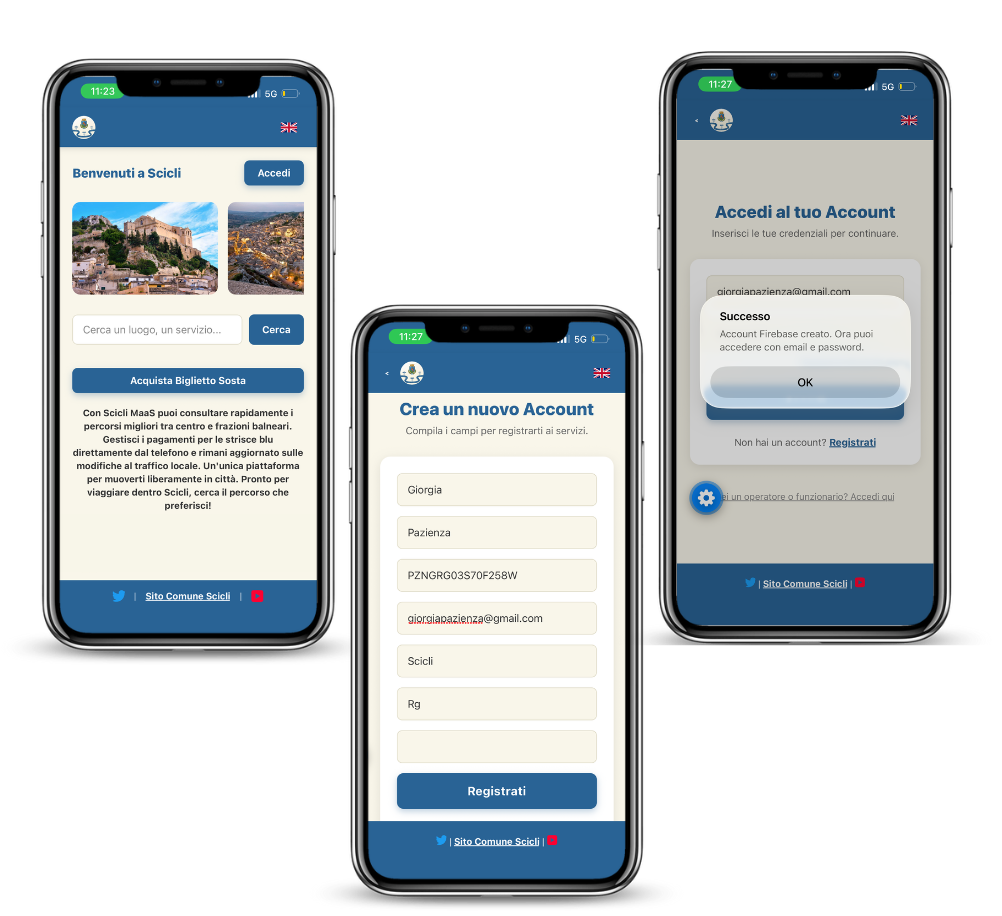
\includegraphics[width=\linewidth]{Foto/Autenticazione.png}
        \caption{}
        \label{fig:test_login}
    \end{minipage}\hfill
    \begin{minipage}{0.5\textwidth}
        \centering
        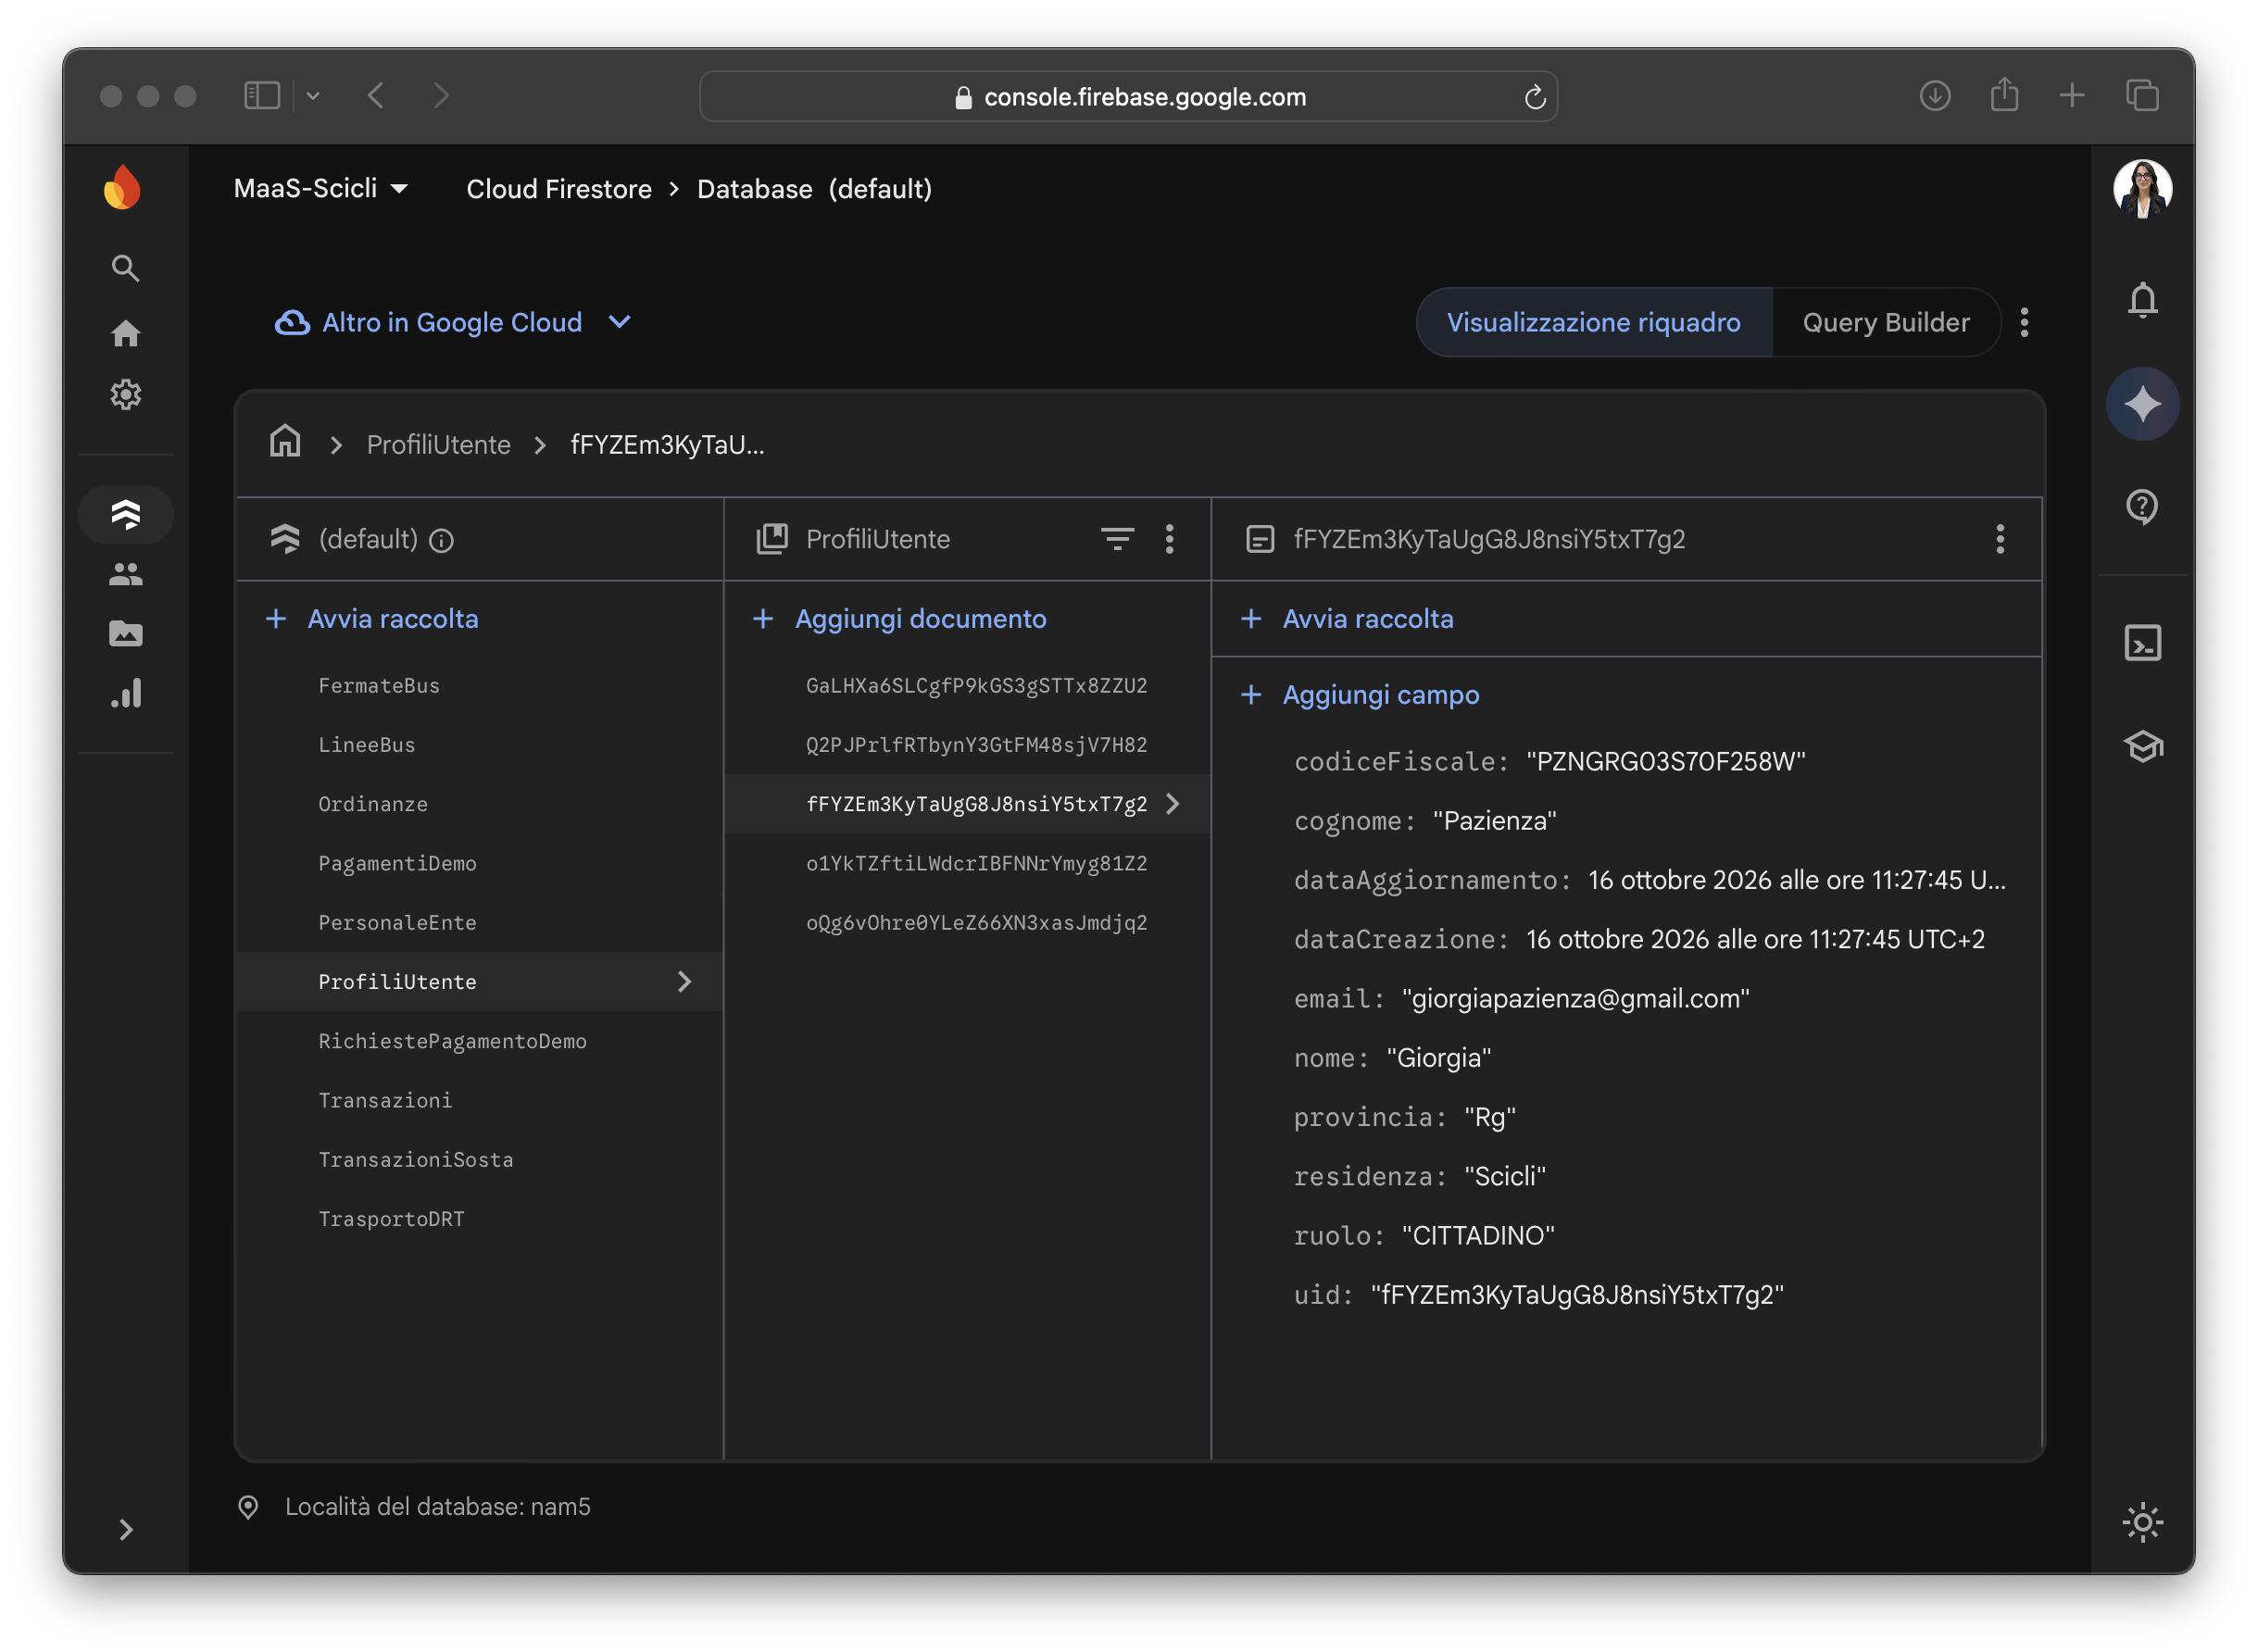
\includegraphics[width=\linewidth]{Foto/image.png}
        \caption{}
        \label{fig:placeholder}
    \end{minipage}
\end{figure}
\noindent
Successivamente, attraverso due schermate dedicate, si procede a testare l'autenticazione per tutti gli attori coinvolti, sia di natura istituzionale che non istituzionale. 
\begin{figure}[H]
    \centering
    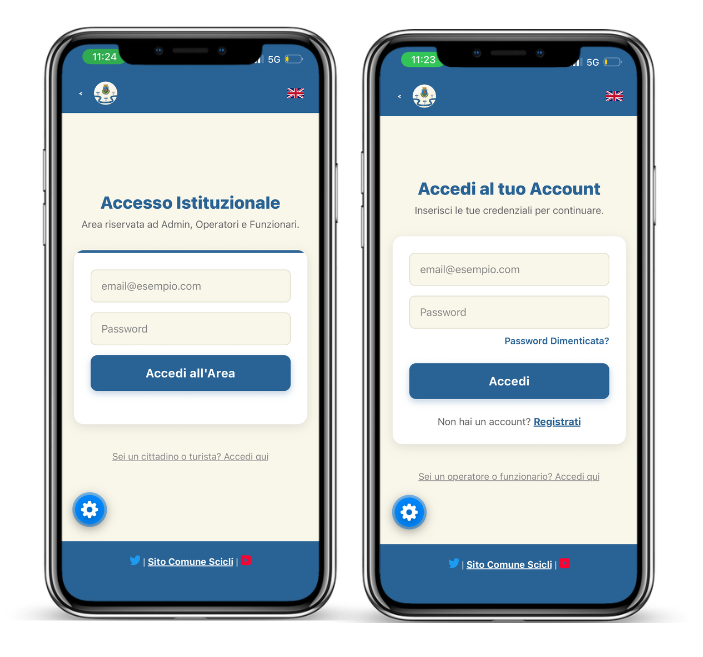
\includegraphics[width=0.5\linewidth]{Foto/Accesso.png}
    \caption{}
    \label{fig:placeholder}
\end{figure}
\noindent
Infine, a seguito della validazione delle credenziali, viene verificata la corretta apertura e il reindirizzamento alle dashboard specifiche in base al ruolo dell'utente.
\begin{figure}[H]
    \centering
    \begin{minipage}{0.5\textwidth}
        \centering
        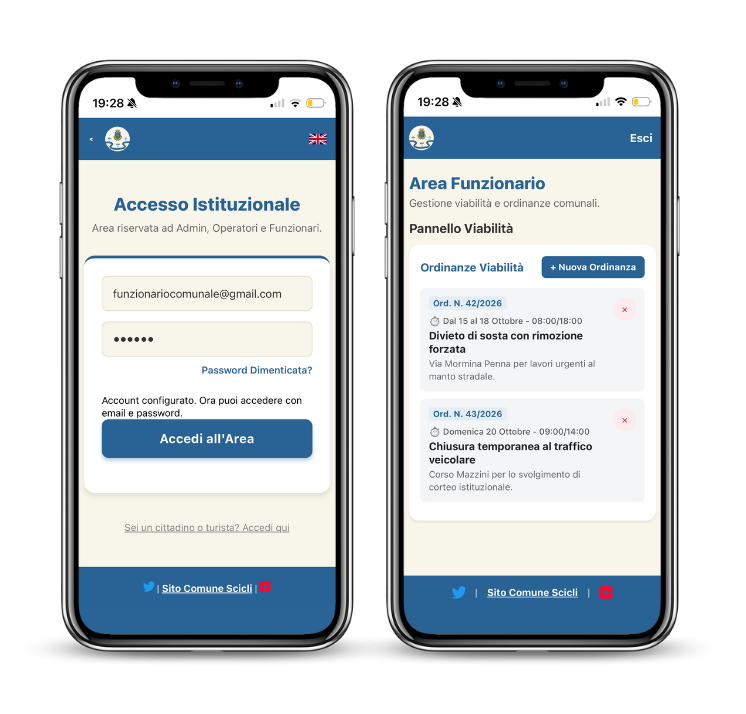
\includegraphics[width=\linewidth]{Foto/Funzionario.png}
        \caption{}
        \label{fig:funzionario}
    \end{minipage}\hfill
    \begin{minipage}{0.5\textwidth}
        \centering
        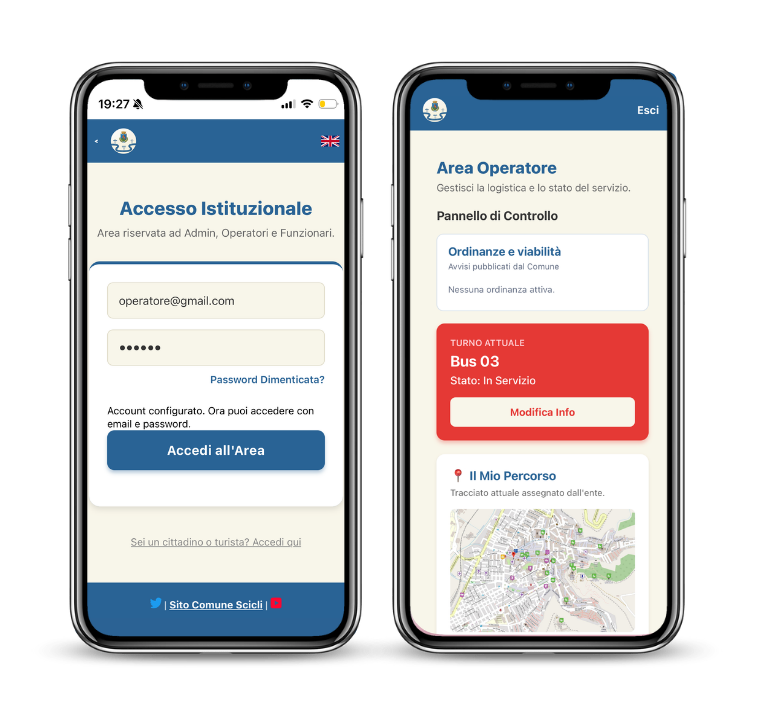
\includegraphics[width=\linewidth]{Foto/Operatore.png}
        \caption{}
        \label{fig:operatore}
    \end{minipage}\hfill
    \begin{minipage}{0.5\textwidth}
        \centering
        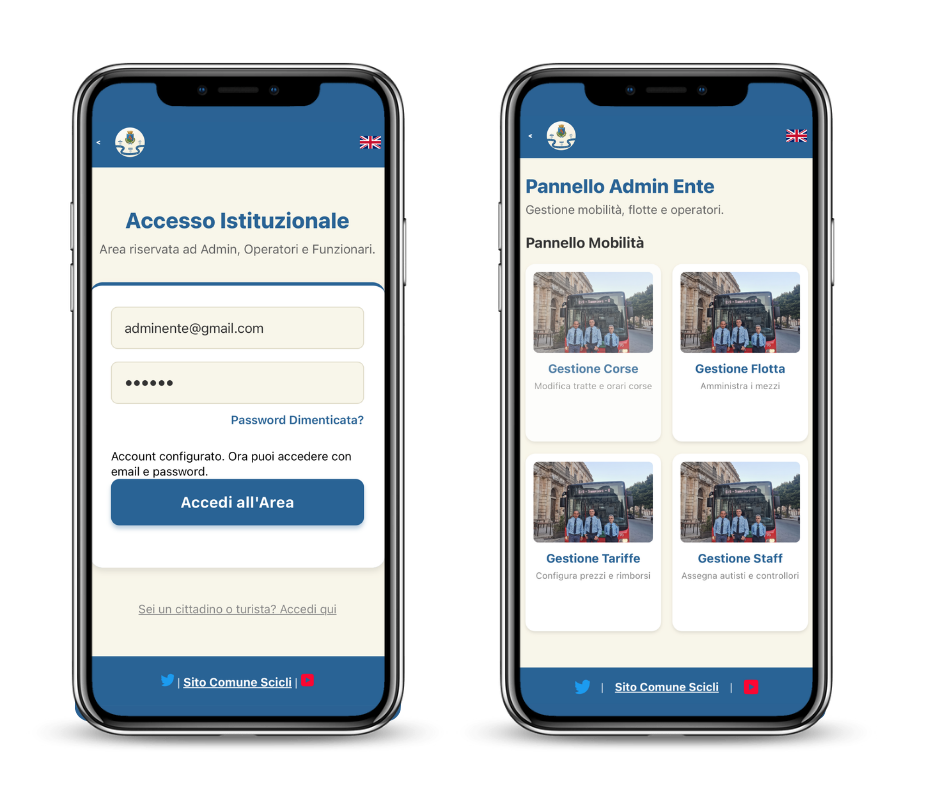
\includegraphics[width=\linewidth]{Foto/AdminEnte.png}
        \caption{}
        \label{fig:admin}
    \end{minipage}\hfill
    \begin{minipage}{0.5\textwidth}
        \centering
        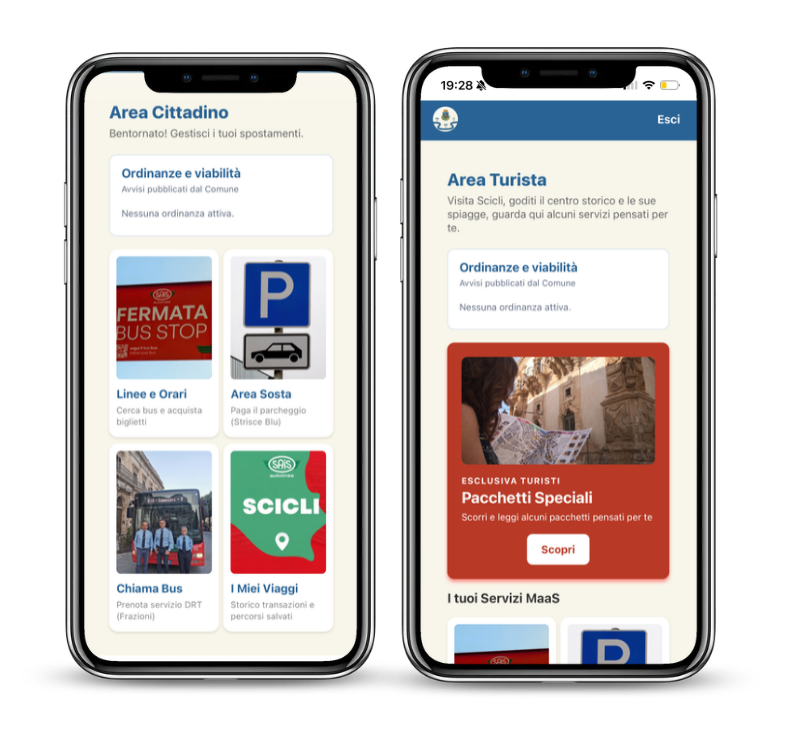
\includegraphics[width=\linewidth]{Foto/DashboardCitt:Tur.png}
        \caption{}
        \label{fig:operatore}
        \end{minipage}
\end{figure}
\noindent
Qualora le credenziali inserite nel pannello di accesso risultino errate, è possibile avviare la procedura di recupero della password tramite l'apposito pulsante, che reindirizza l'utente alla schermata dedicata.
\begin{figure}[H]
    \centering 
    \begin{minipage}{0.3\textwidth}
        \centering 
        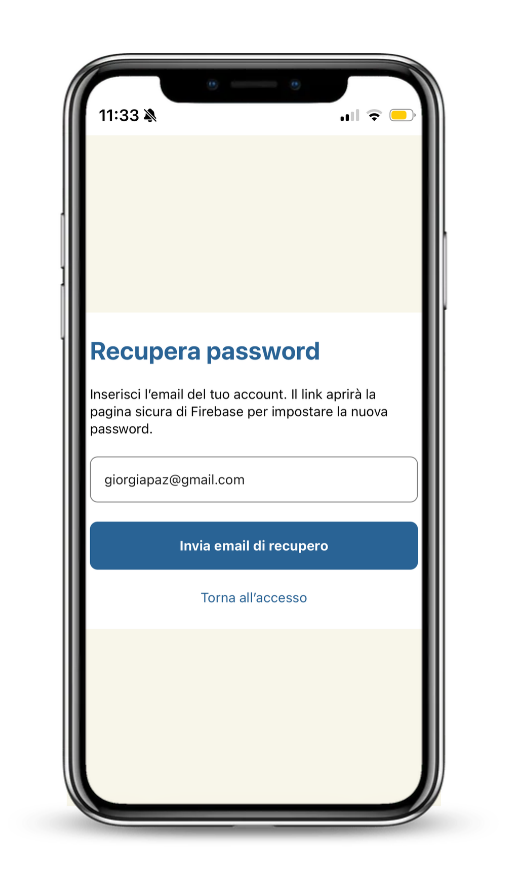
\includegraphics[width=\linewidth]{Foto/Recupera_Password.png}
        \caption{}
        \label{fig:operatore}
    \end{minipage}
\end{figure}
\noindent
\textbf{Consultazione Mobilità e Ricerca Percorsi:} In questa fase è stata testata la funzionalità di ricerca delle tratte, verificando che il sistema restituisca correttamente gli orari e le fermate in base ai parametri inseriti dall'utente.
\begin{figure}[H]
    \centering
    \includegraphics[width=0.5\textwidth]{Foto/ConsultazioneMobilità.png}
    \caption{}
    \label{fig:test_ricerca}
\end{figure}
\noindent
\textbf{Prenotazione Servizio DRT (Trasporto a Chiamata):}
Il modulo DRT mostra la capacità del sistema di registrare una nuova richiesta di trasporto per le frazioni periferiche e di inviare correttamente la notifica al pannello dell'Operatore, aggiornando i dati pure sul database Firebase.
\begin{figure}[H]
    \centering
    \begin{minipage}{0.5\textwidth}
        \centering
        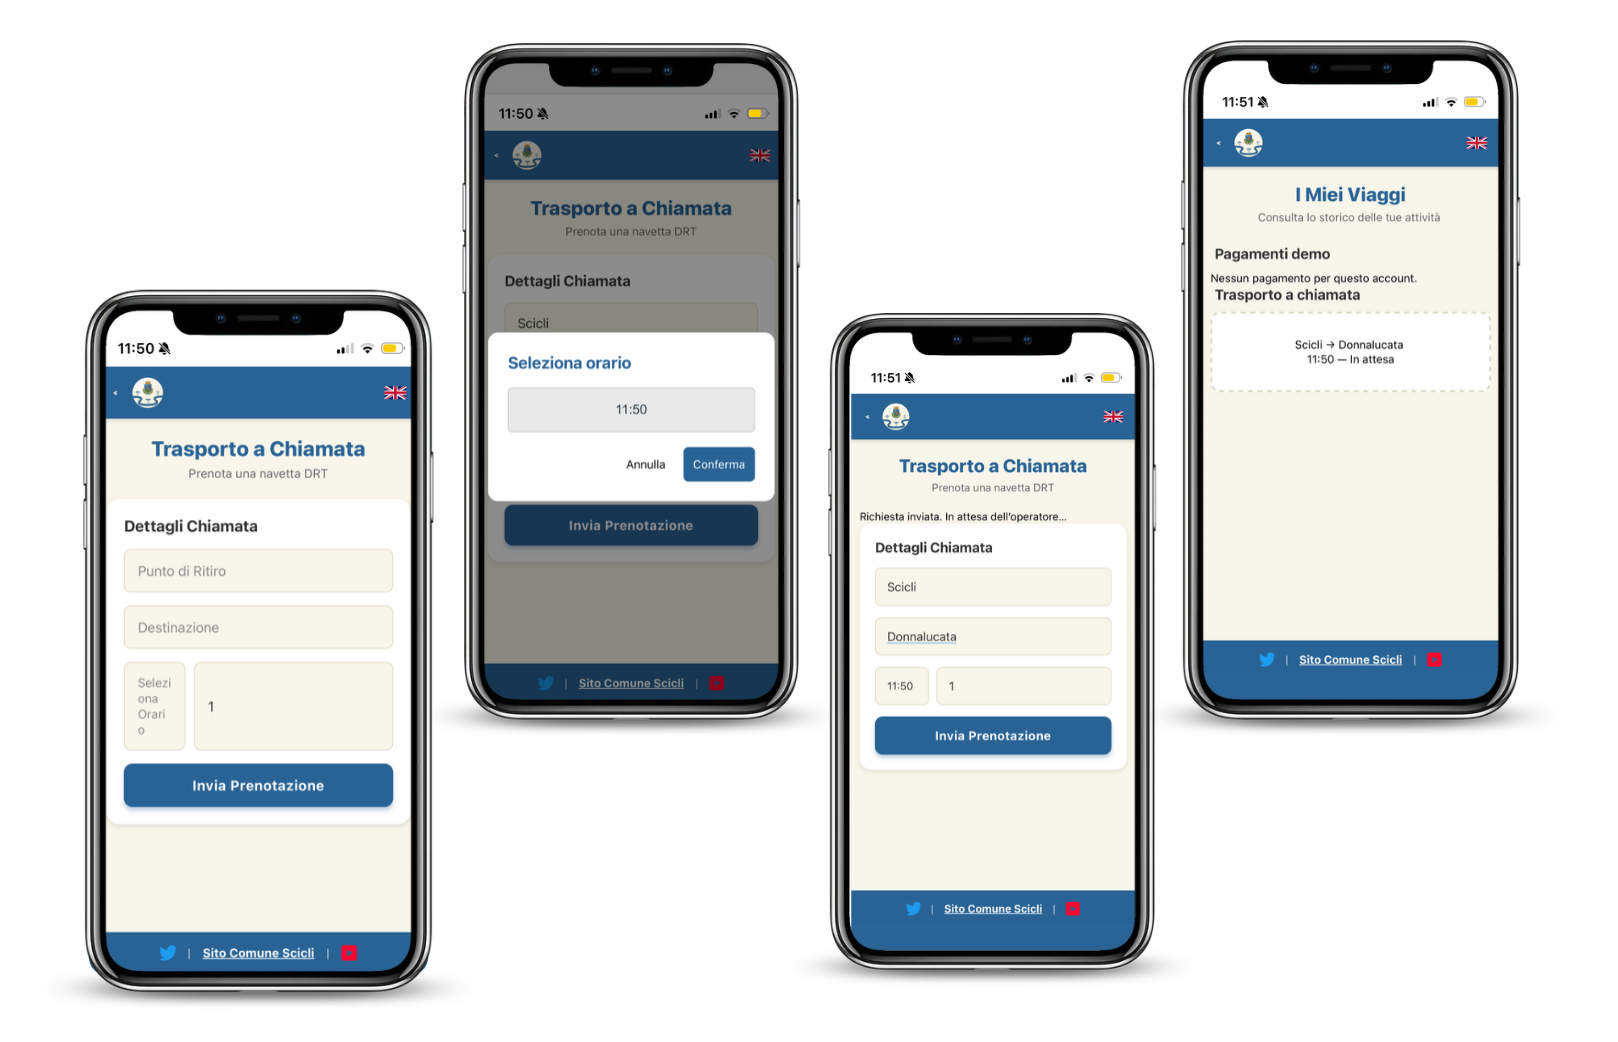
\includegraphics[width=\textwidth]{Foto/TrasportoChiamata.png}
        \caption{}
        \label{fig:test_drt_chiamata}
    \end{minipage}\hfill
    \begin{minipage}{0.5\textwidth}
        \centering
        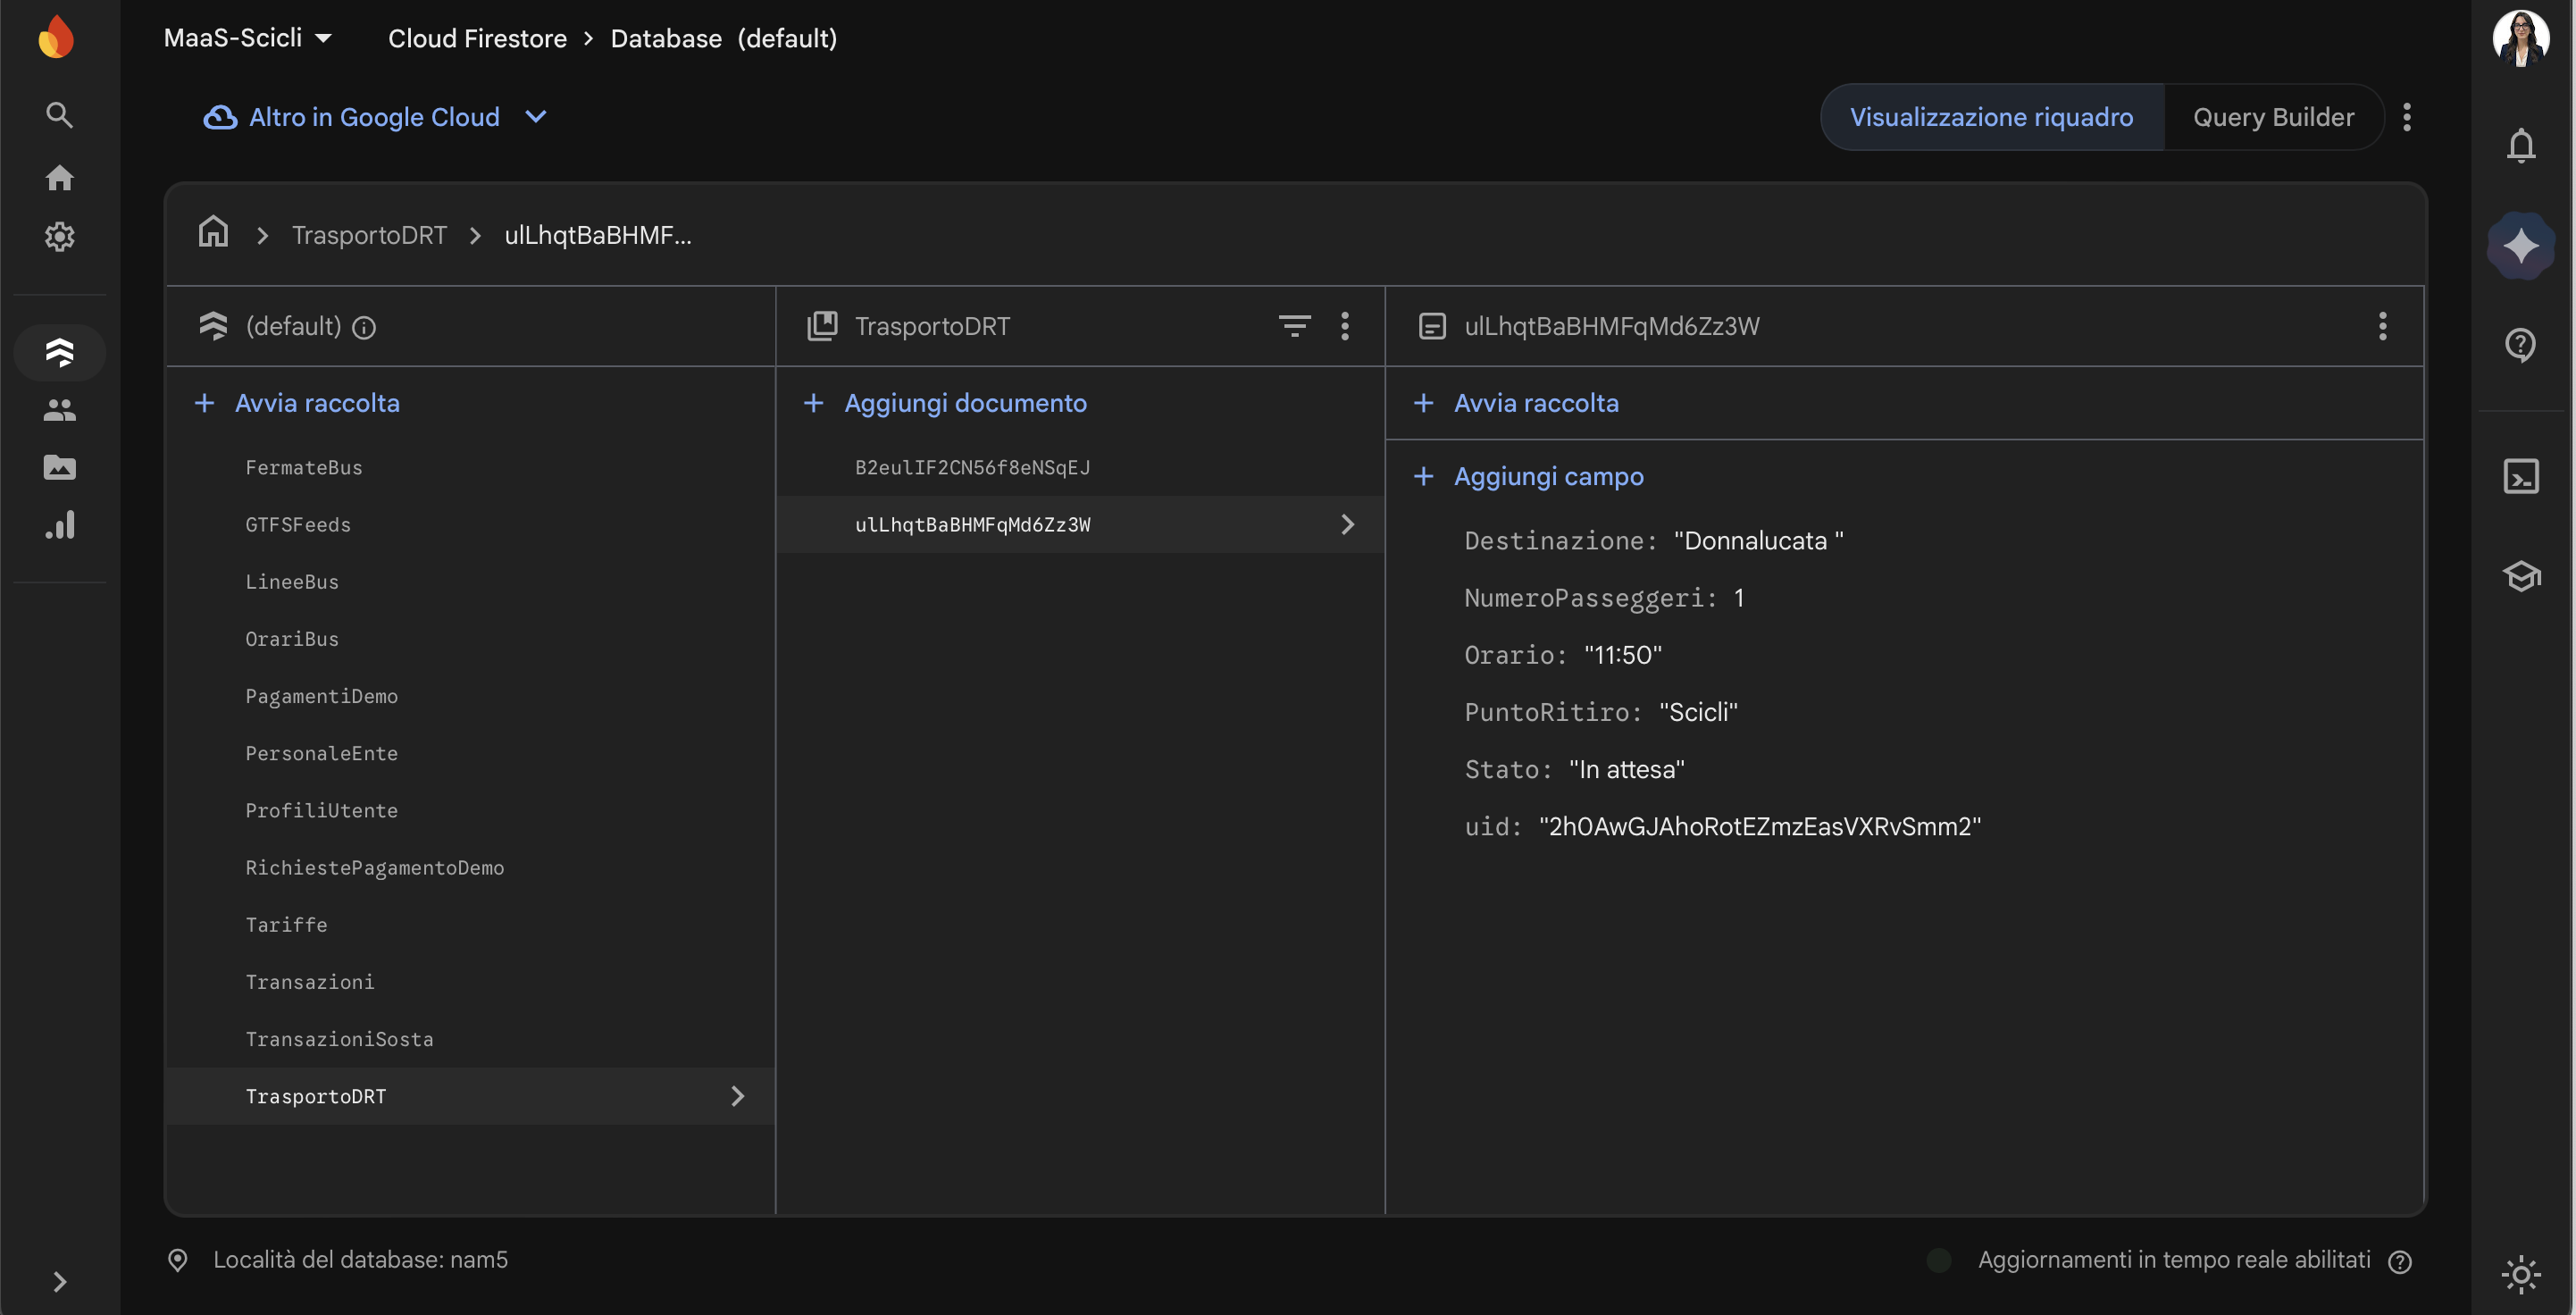
\includegraphics[width=\textwidth]{Foto/FirestoreDRT.png}
        \caption{}
        \label{fig:test_drt_firestore}
    \end{minipage}
\end{figure}
\noindent
\textbf{Acquisto Titoli di Viaggio e Pagamento Sosta: }
Un aspetto critico del testing riguarda il modulo dei pagamenti simulati. È stato verificato il corretto funzionamento del wallet digitale, accertando che l'acquisto di un biglietto o il pagamento delle strisce blu generi correttamente la transazione e aggiorni lo storico dell'utente.
\begin{figure}[H]
    \centering
    
    % --- PRIMA RIGA ---
    \begin{minipage}{0.55\textwidth}
        \centering
        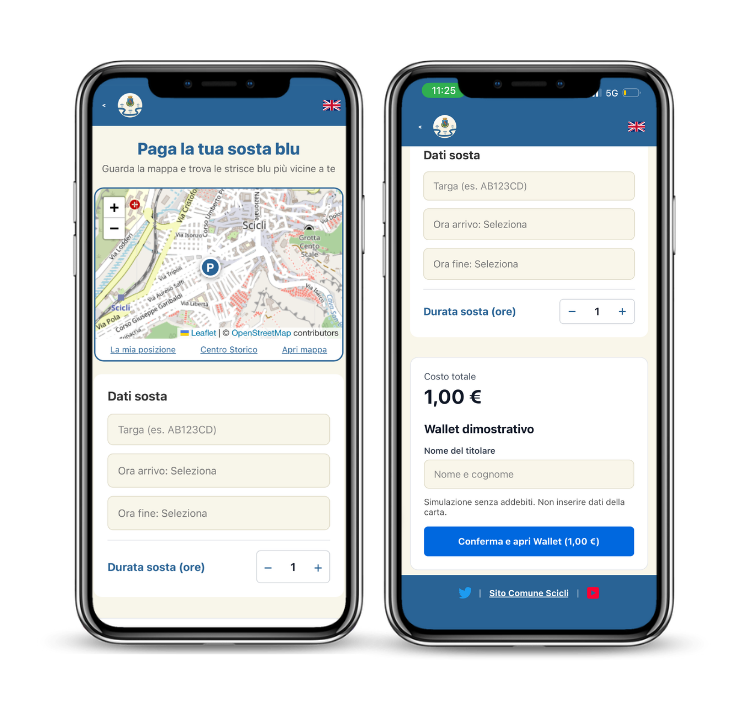
\includegraphics[width=\linewidth]{Foto/Sosta.png}
        \caption{}
        \label{fig:test_pagamento_1}
    \end{minipage}\hfill
    \begin{minipage}{0.35\textwidth}
        \centering
        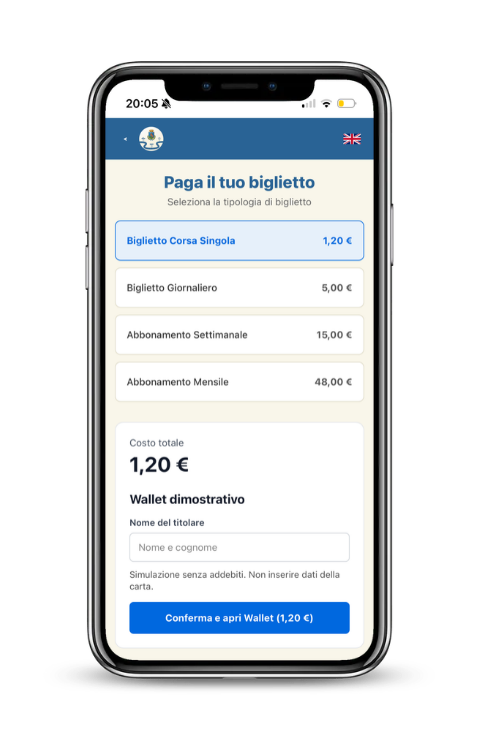
\includegraphics[width=\linewidth]{Foto/BigliettoBus.png}
        \caption{}
        \label{fig:test_pagamento_2}
    \end{minipage}
    \vspace{1cm} 
    \begin{minipage}{0.45\textwidth}
        \centering
        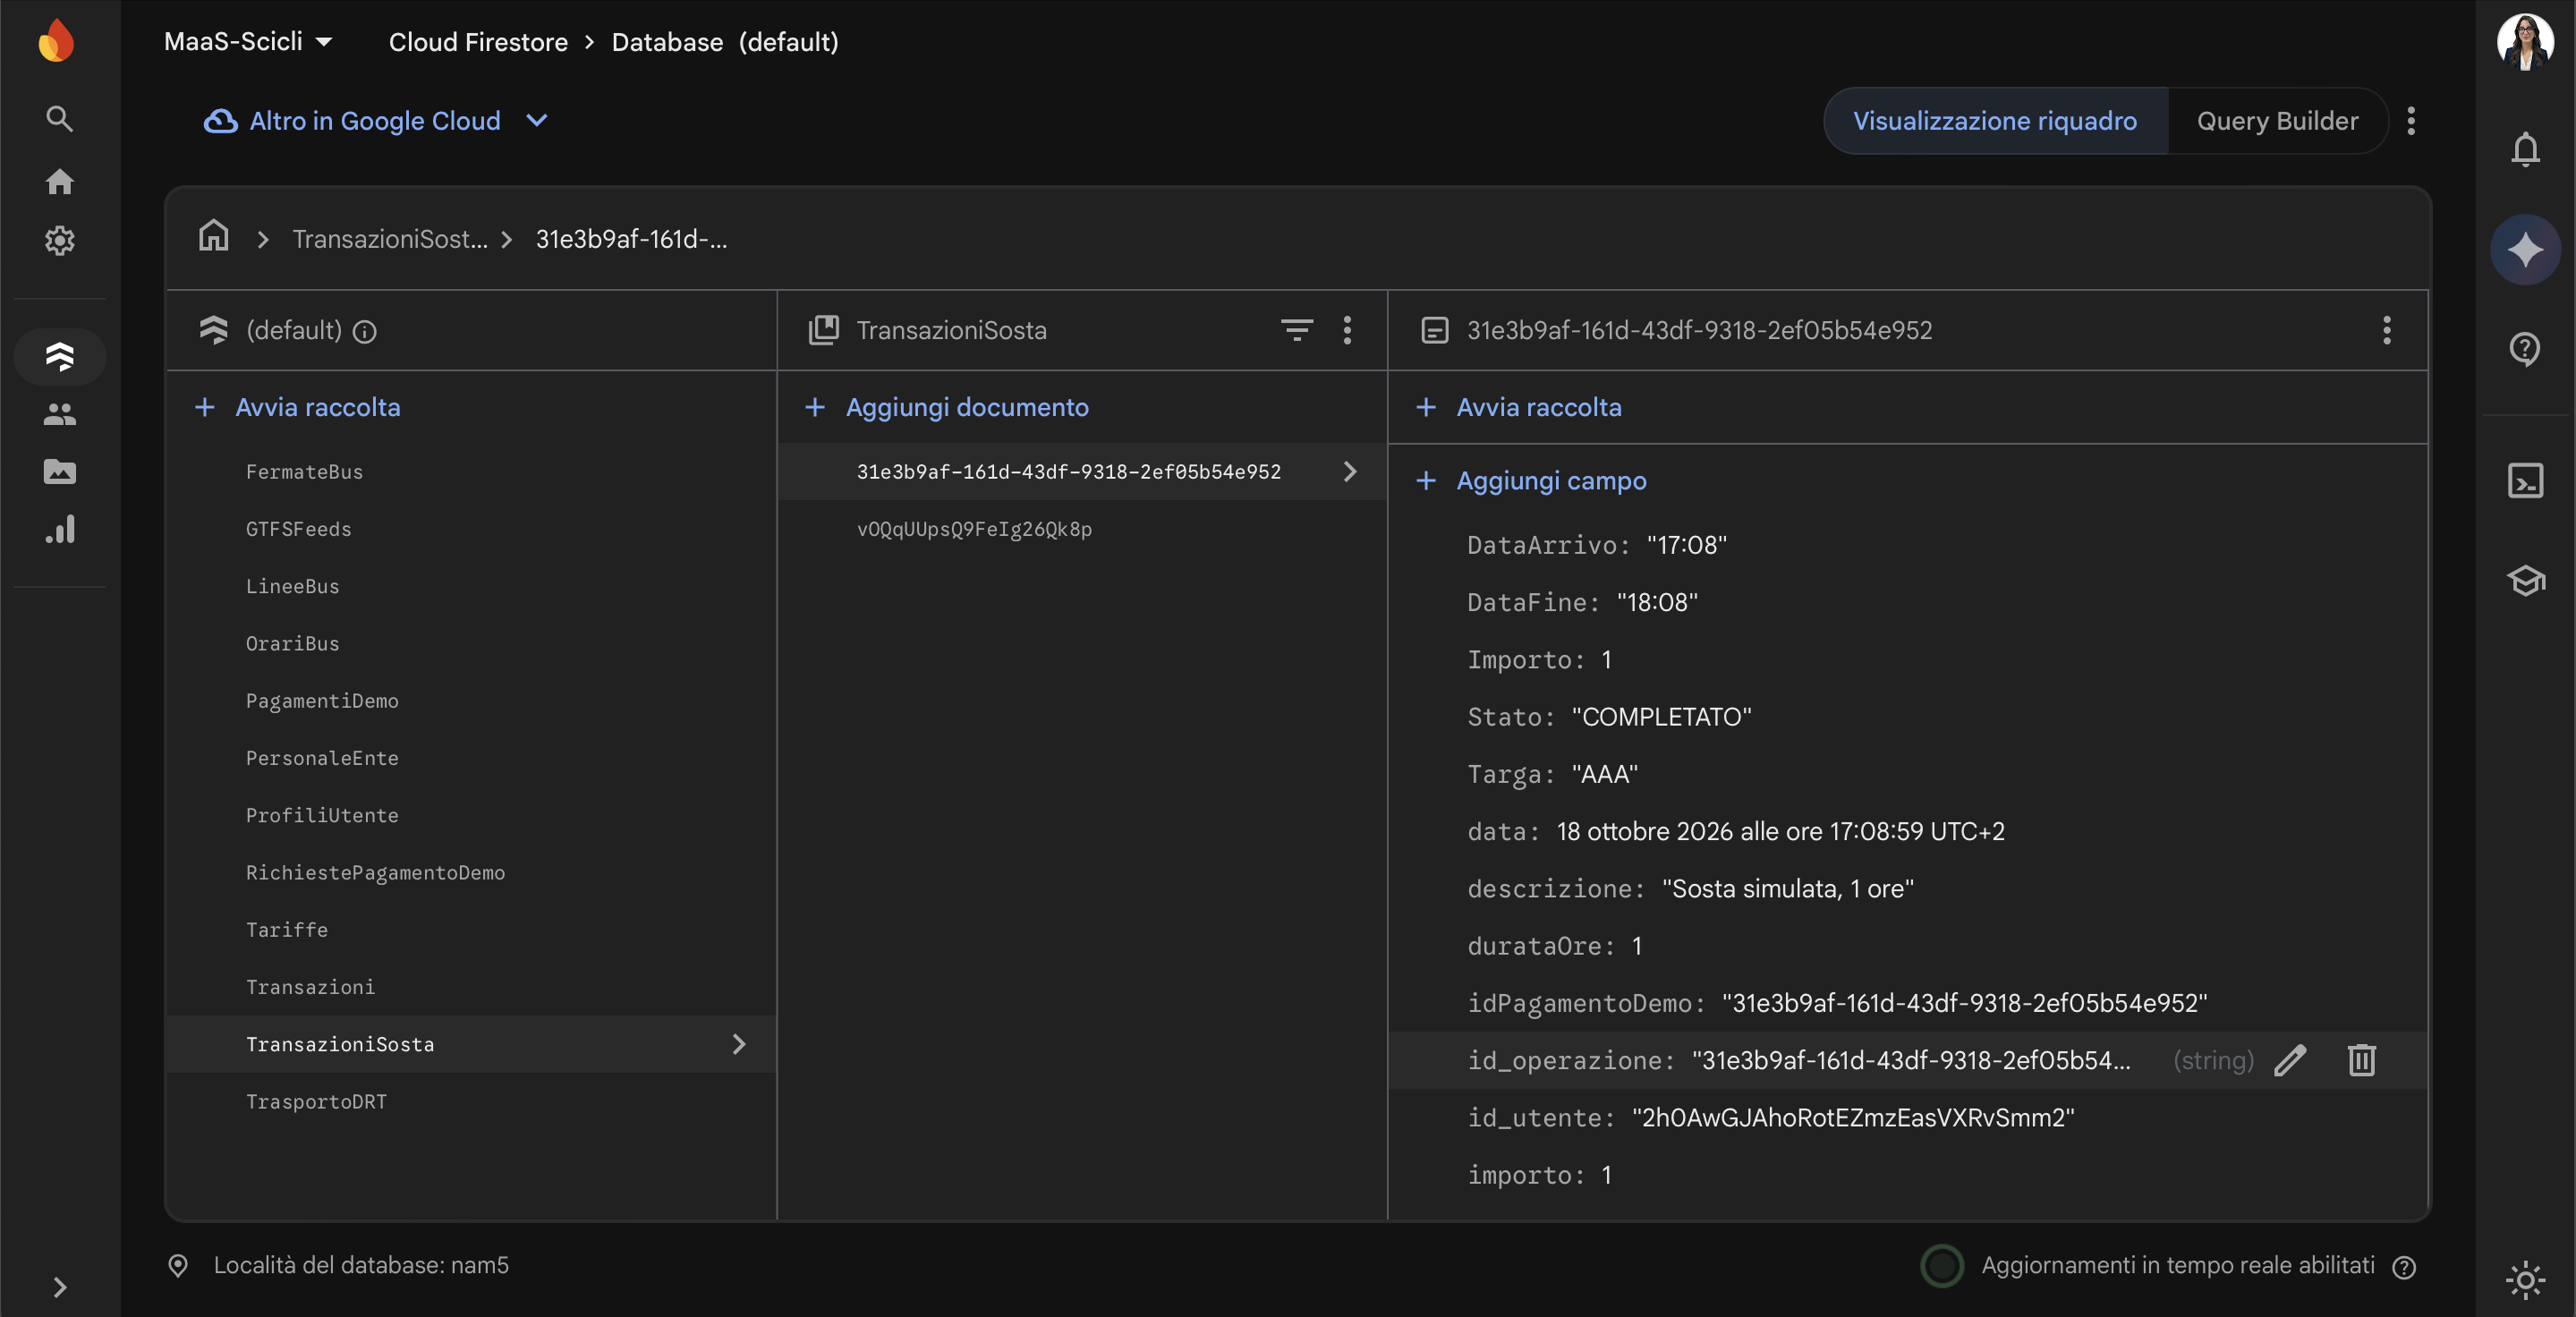
\includegraphics[width=\linewidth]{Foto/Transazioni Sosta.png}
        \caption{}
        \label{fig:test_transazioni_sosta}
    \end{minipage}\hfill 
    \begin{minipage}{0.45\textwidth}
        \centering
        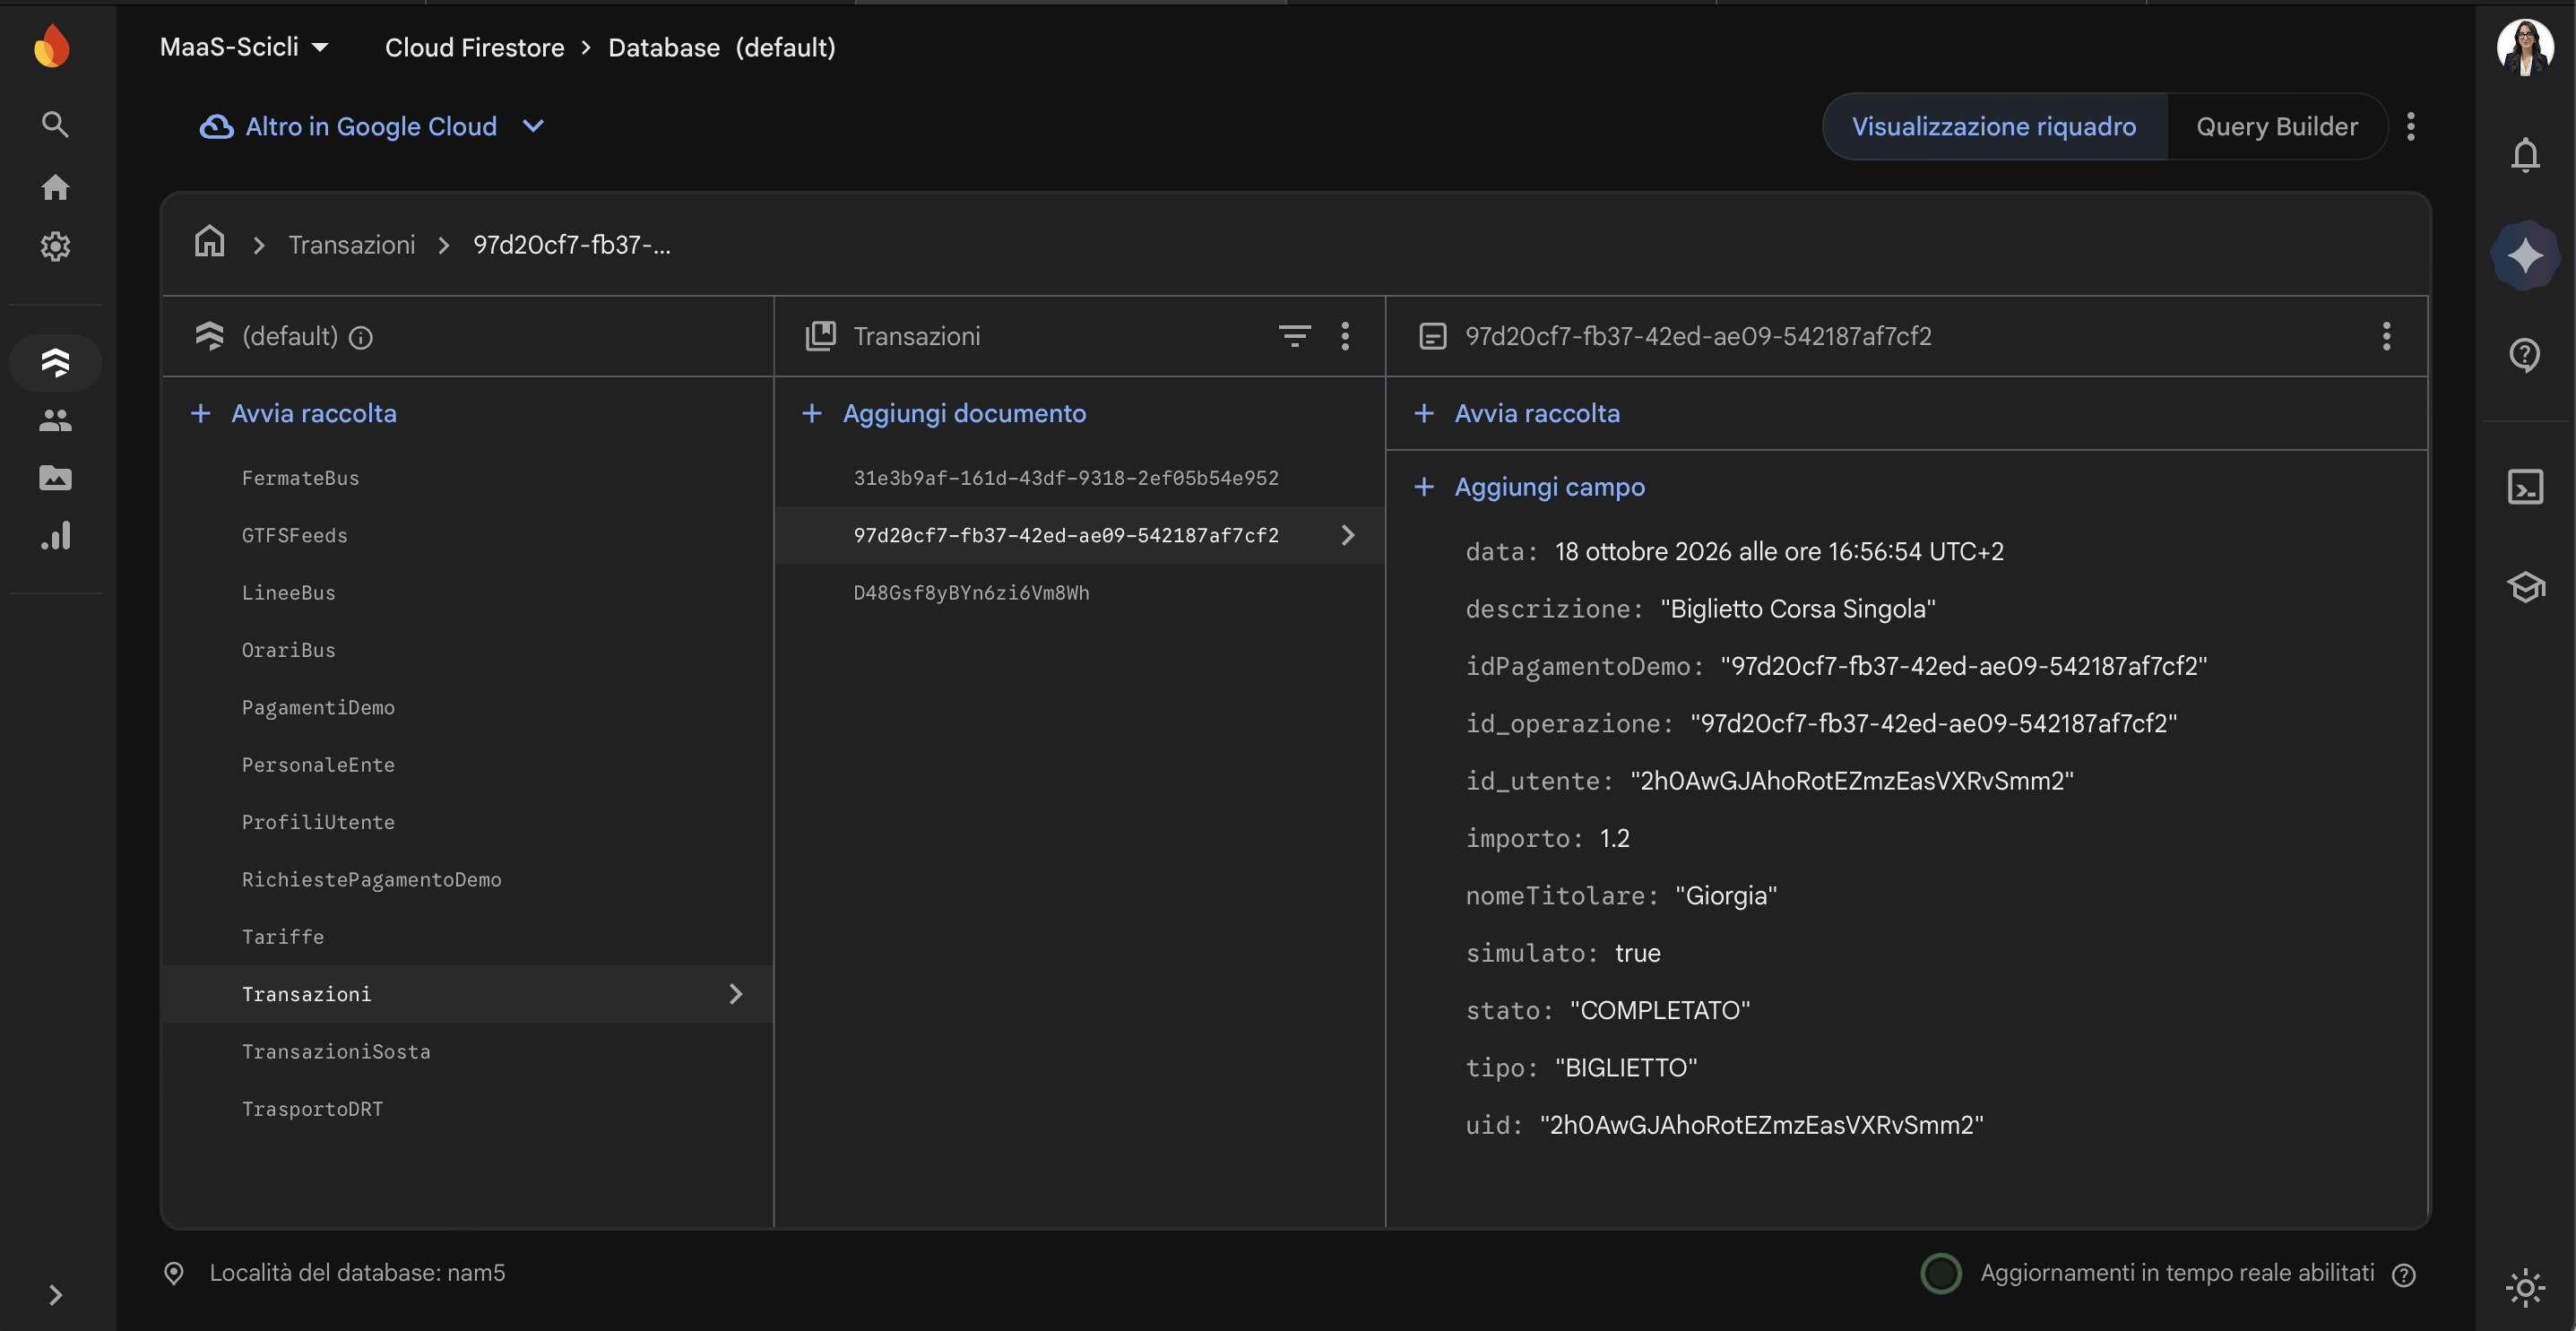
\includegraphics[width=\linewidth]{Foto/TransazioniBiglietto.png}
        \caption{}
        \label{fig:test_transazioni_biglietti}
    \end{minipage}
\end{figure}
\begin{figure}[H]
    \centering
    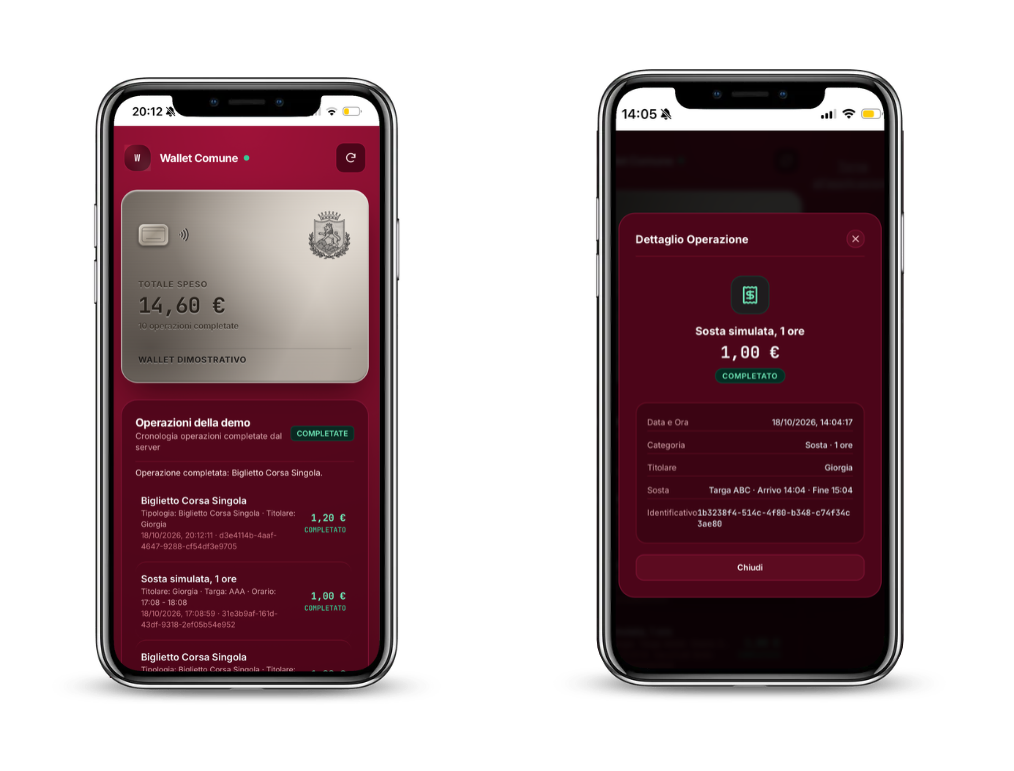
\includegraphics[width=0.7\linewidth]{Foto/Wallet.png}
    \caption{}
    \label{fig:placeholder}
\end{figure}
\noindent
\textbf{Pannello Admin e Gestione Staff:}
Un ulteriore test è stato condotto sull'interfaccia riservata all'Admin dell'Ente.
Il test ha confermato che l'Admin è in grado di visualizzare l'anagrafica, assegnare i turni e monitorare gli operatori attivi all'interno del sistema.
\begin{figure}[H]
    \centering
    \begin{minipage}{0.25\textwidth}
        \centering
        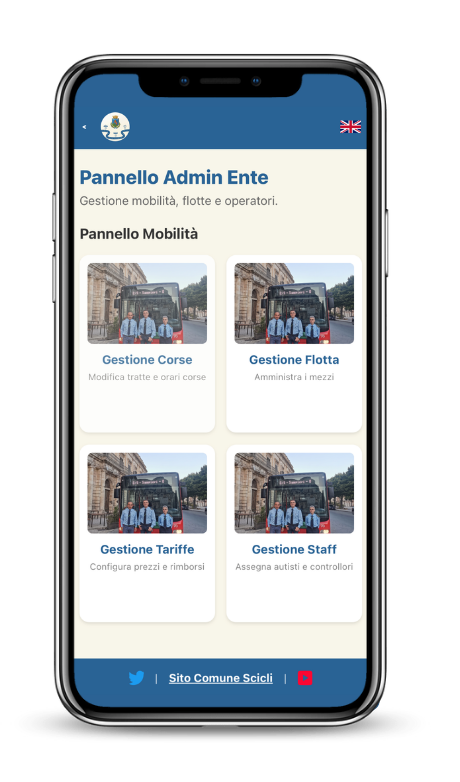
\includegraphics[width=\linewidth]{Foto/PannelloAdmin.png}
        \caption{}
        \label{fig:test_pagamento_1}
    \end{minipage}\hfill
    \begin{minipage}{0.75\textwidth}
        \centering
        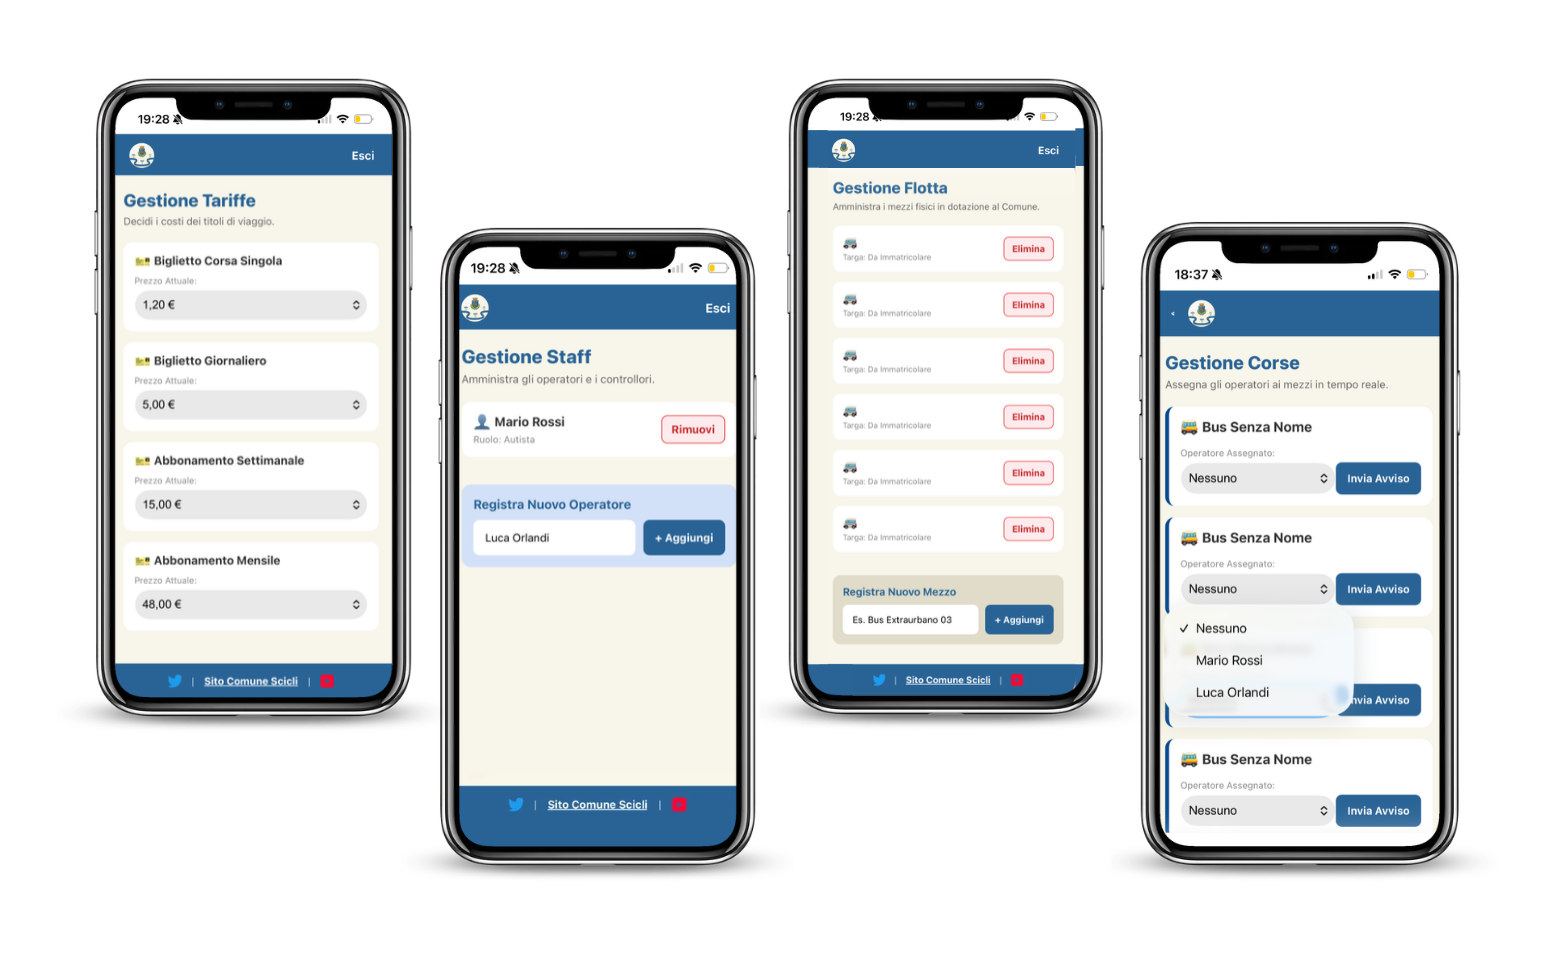
\includegraphics[width=\linewidth]{Foto/PannelloA.png}
        \caption{}
        \label{fig:test_pagamento_2}
    \end{minipage}
\end{figure}
\noindent
\textbf{Funzionario Comunale e Gestione Ordinanze:}
Per quanto riguarda le figure istituzionali, è stato simulato il flusso operativo del Funzionario Comunale. Il test ha validato la procedura di caricamento e pubblicazione di una nuova ordinanza relativa alla viabilità. Si è verificato che il documento venga correttamente elaborato e che gli alert risultino visibili sulla mappa e notificati agli enti interessati.
\begin{figure}[H]
    \centering
    \begin{minipage}{0.5\textwidth}
        \centering
        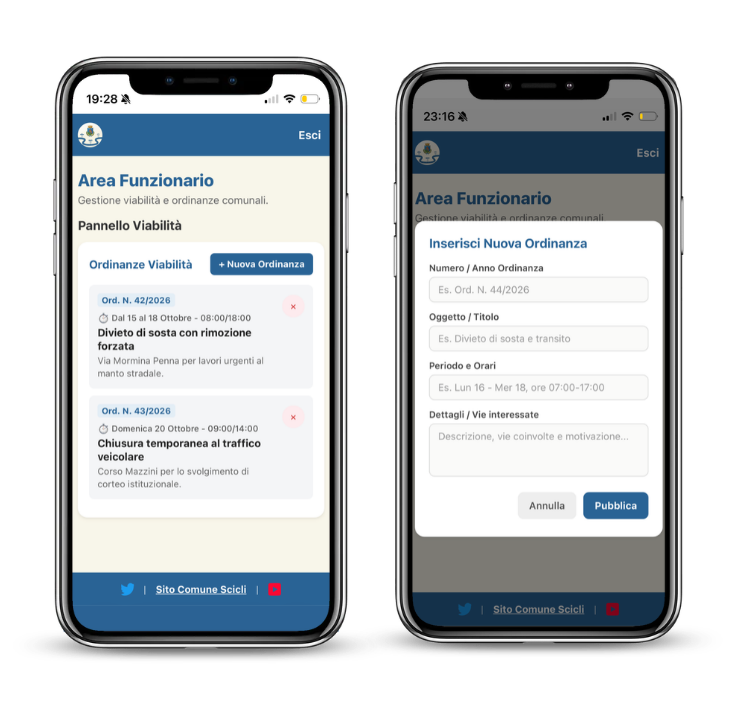
\includegraphics[width=\linewidth]{Foto/Ordinanza.png}
        \caption{}
        \label{fig:test_ordinanze_1}
    \end{minipage}\hfill
    \begin{minipage}{0.5\textwidth}
        \centering
        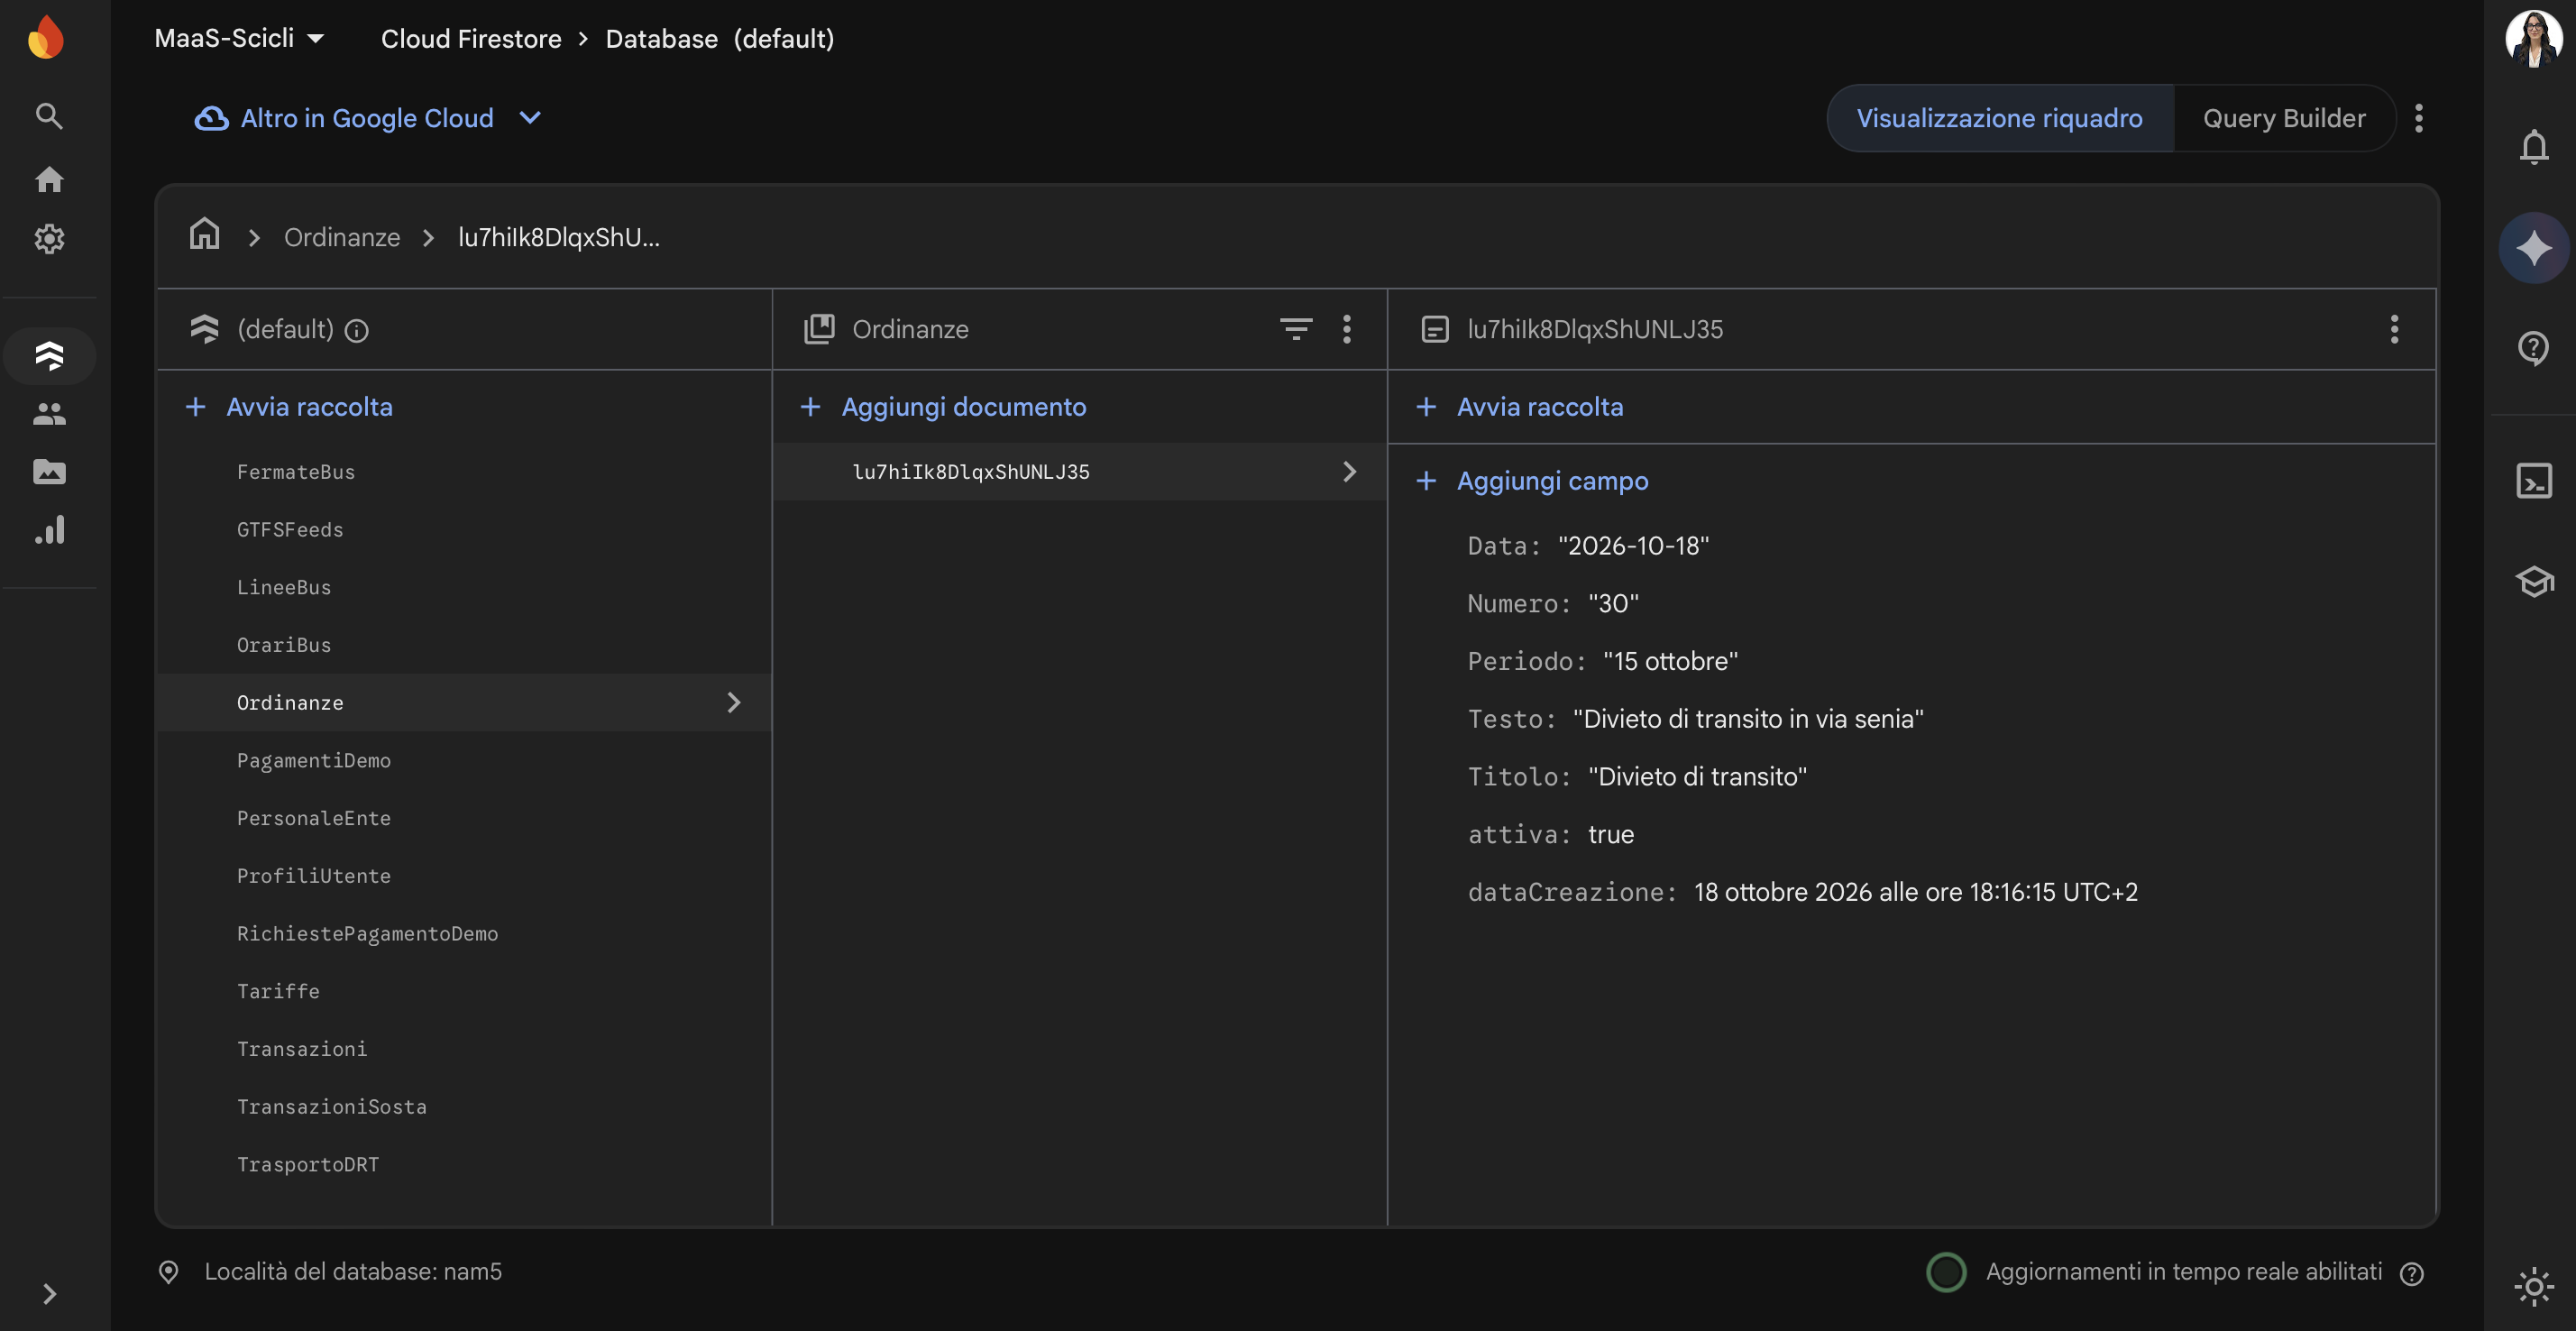
\includegraphics[width=\linewidth]{Foto/Ordinanze.png}
        \caption{}
        \label{fig:test_ordinanze_2}
    \end{minipage}
\end{figure}
\noindent
I test eseguiti hanno dimostrato la stabilità generale del prototipo. Le chiamate alle API REST e le interazioni con il database NoSQL hanno mostrato tempi di risposta adeguati. L'interfaccia utente è risultata reattiva e coerente con i casi d'uso progettati nella fase di analisi, confermando la fattibilità del modello MaaS per la digitalizzazione dei trasporti nel territorio analizzato.
\newpage

\chapter{Conclusioni e Sviluppi Futuri}

\section{Riepilogo del lavoro}
Il presente lavoro di tesi ha affrontato l'analisi, la progettazione e la realizzazione prototipale di una piattaforma informatica ispirata al paradigma \emph{Mobility as a Service} (MaaS), con l'obiettivo di delineare un punto di accesso unitario a differenti servizi di mobilità riferiti al territorio del Comune di Scicli. La proposta nasce dall'esigenza di ricondurre in un un'unica applicazione le operazioni di spostamento all'interno del comune, anche se considerate separatamente, possono risultare difficili da consultare e utilizzare.
\\
Il contesto territoriale ha costituito un elemento determinante nelle scelte progettuali. Il rapporto tra il centro urbano e le frazioni costiere, fra cui Donnalucata, Arizza, Sampieri e Cava d'Aliga, pone infatti questioni di accessibilità e collegamento che possono assumere caratteristiche differenti durante l'anno. La concentrazione stagionale dei flussi turistici rende particolarmente importante la disponibilità di informazioni comprensibili e aggiornate, mentre nei periodi caratterizzati da una domanda più contenuta diviene rilevante valutare forme di trasporto flessibile. In questo quadro, il paradigma MaaS è stato assunto non come una singola tecnologia, bensì come un criterio di integrazione dei servizi e di semplificazione dell'esperienza dell'utente.
\\
Il percorso seguito si è articolato in fasi logicamente connesse. L'analisi iniziale ha permesso di individuare gli attori coinvolti, le operazioni richieste e i principali vincoli del dominio applicativo. La successiva progettazione, supportata da strumenti di modellazione \emph{Unified Modeling Language} (UML), ha definito i casi d'uso e le interazioni fra componenti mediante diagrammi di attività e di sequenza. 
\\
A partire da tali risultati, è stata sviluppata un'architettura ibrida che integra un frontend mobile in React Native, un backend Java Spring Boot, servizi BaaS Firebase per autenticazione e dati, e un database relazionale separato per la gestione dei percorsi GTFS

\section{Sviluppi futuri}
La progettazione dell'applicativo pone delle basi solide per un'espansione del sistema. Al fine di rendere la piattaforma uno strumento sempre più avanzato si propongono di seguito le principali idee per alcuni futuri sviluppi.
\subsection*{Consolidamento dell'architettura e interoperabilità dei dati}
Le future linee di intervento mirano innanzitutto a stabilizzare l'architettura ibrida, spostando le operazioni più delicate, come quelle amministrative o soggette a vincoli, direttamente sul server. L'accesso diretto al database dal client verrà mantenuto solo dove la sincronizzazione in tempo reale è davvero necessaria, tutelandolo con adeguate regole di sicurezza.
\\
Parallelamente, si rende necessaria l'introduzione di modelli dati condivisi e controlli semantici per prevenire incongruenze informative tra i vari livelli applicativi. 
\\
In ambito trasporti, ciò si traduce in un processo strutturato per l'importazione dei dati GTFS, essenziale per distinguere la programmazione statica dagli effettivi aggiornamenti in tempo reale. Un'ulteriore estensione riguarderà la gestione delle aree di parcheggio a pagamento: sarà necessario integrare fonti dati georeferenziate, attualmente mancanti, per consentire la selezione visiva delle strisce blu direttamente dalla mappa. Infine, per favorire l'interoperabilità con enti e operatori esterni, è opportuno definire un set di API stabili e versionate; affinché l'integrazione tecnica sia efficace, essa dovrà tuttavia essere supportata da precisi accordi organizzativi volti a certificare la qualità e l'affidabilità delle informazioni erogate all'utente.
\\
\subsection*{Ottimizzazione logistica tramite Teoria dei Grafi}
Un'evoluzione interessante riguarda l'impiego di algoritmi per la ricerca e l'ottimizzazione dei percorsi. Modellando la rete della città di Scicli come un grafo pesato: può essere rappresentata mediante un grafo orientato e pesato $G=(V,E)$, nel quale l'insieme $V$ comprende fermate e nodi rilevanti della rete urbana, mentre $E$ rappresenta i collegamenti percorribili. A ciascun arco $e\in E$ è associato un peso non negativo $w(e)$, interpretabile, ad esempio, come tempo di percorrenza stimato. Il costo complessivo di un cammino $P$ risulta pertanto:
\begin{equation}
    C(P)=\sum_{e\in P} w(e),
    \label{eq:costo_percorso}
\end{equation}
\vspace{1em}
Per poi successivamente utilizzare algoritmi di ricerca e calcolo del percorso minimo, come l'algoritmo di Dijkstra o altri. Questo approccio permetterebbe di ottimizzare le risorse, riducendo i chilometri percorsi a vuoto e migliorando i tempi di attesa per gli utenti.

\subsection*{Integrazione di Intelligenza Artificiale e NLP}
Una seconda prospettiva di sviluppo riguarda l'introduzione di un assistente virtuale in grado di semplificare l'accesso alle informazioni e alle operazioni più comuni. Attraverso tecniche di \emph{Natural Language Processing} (NLP), l'utente potrebbe formulare richieste in linguaggio naturale, senza dover conoscere in anticipo la collocazione delle singole funzioni nell'interfaccia. 
Un visitatore, per esempio, potrebbe chiedere quale collegamento sia disponibile tra il centro di Scicli e una località costiera, ricevere chiarimenti sui servizi di trasporto oppure ottenere indicazioni sull'esistenza di eventuali limitazioni alla circolazione.
\\
Per contenere il rischio di fornire informazioni non aggiornate, l'assistente potrebbe adottare un approccio \emph{Retrieval-Augmented Generation} (RAG), nel quale la generazione della risposta è supportata dal recupero di contenuti provenienti da fonti selezionate. Nel contesto del progetto, le fonti potrebbero comprendere descrizioni dei servizi, ordinanze pubblicate, informazioni validate sulle fermate e disponibilità del DRT, purché rese accessibili attraverso un livello applicativo controllato. 

\subsection*{Sicurezza Informatica e Protezione dei Dati pèrsonali}
Considerando la mole di dati sensibili trattati, legati alla geolocalizzazione degli utenti e alle transazioni finanziarie, un focus primario dovrà essere dedicato alla \textit{CSicurezza Informatica}. 
\\
A livello tecnico, sarà fondamentale proteggere le comunicazioni mediante protocolli crittografici robusti (come HTTPS/TLS per i dati in transito) e implementare meccanismi di difesa contro attacchi esterni, quali i DDoS. Parallelamente, le logiche di accesso dovranno essere rafforzate sia sugli endpoint del server Spring Boot, sia sulle regole di sicurezza di Firestore. L'obiettivo è applicare rigorosamente il principio del \emph{privilegio minimo}, verificando sempre lato server le credenziali e assicurando che ogni utente o servizio acceda esclusivamente alle risorse per cui è esplicitamente autorizzato.
\\
Sul versante della tutela della privacy, il sistema dovrà garantire la piena conformità al Regolamento Europeo (GDPR). Ciò si traduce nell'adozione di un approccio \emph{privacy by design}, implementando rigidi protocolli di minimizzazione e pseudonimizzazione dei dati personali. Queste misure, supportate da una gestione sicura dei segreti applicativi e da un monitoraggio continuo degli accessi, risultano essenziali per mitigare i rischi e offrire all'utente un ambiente digitale affidabile e protetto.

\subsection*{Evoluzione dei Sistemi di Pagamento}
La gestione dei pagamenti costituisce un'area di evoluzione significativa, poiché il prototipo dispone attualmente di flussi dimostrativi, utili a descrivere il ciclo di vita di un'operazione ma non equivalenti a una transazione economica effettiva. Il passaggio a un ambiente produttivo richiederebbe una separazione netta tra creazione della richiesta di pagamento, esecuzione attraverso un soggetto abilitato, acquisizione dell'esito, registrazione contabile ed eventuali procedure di annullamento o rimborso.
\\
Considerando la destinazione del sistema a un Ente pubblico italiano, l'evoluzione dell'architettura richiederà obbligatoriamente l'integrazione con il nodo pagoPA, in conformità alle direttive dell'Agenzia per l'Italia Digitale (AgID). A tale infrastruttura istituzionale si dovrebbe affiancare il supporto ai principali portafogli digitali (\textit{digital wallet} come Apple Pay e Google Pay), al fine di ottimizzare i tempi di transazione e migliorare l'esperienza d'uso, con particolare beneficio per l'utenza turistica e occasionale.

\section{Conclusioni}
In conclusione, il sistema MaaS creato per la città di Scicli rappresenta una \emph{base prototipale per l'integrazione digitale della mobilità locale}, dalla quale è possibile sviluppare una piattaforma progressivamente più completa. Il contributo della tesi consiste nell'aver trasformato un insieme eterogeneo di esigenze territoriali in un modello funzionale e in un'architettura software concreta, evidenziandone opportunità, limiti e possibili percorsi di evoluzione. La prospettiva di un futuro impiego operativo resta subordinata alla qualità dei dati, alla sicurezza, alla validazione dei processi e alla collaborazione tra amministrazione, operatori e utenti finali.


\newpage

\section*{Ringraziamenti} 
Eccoci qui. In un normale venerdì, dove tutto è finito. Nel momento che aspettavate tutti, quello che qualcuno definirebbe «instagrammabile», l'attimo in cui tutti tirano fuori il telefono per fare foto e video.
Oggi, proprio adesso, vorrei chiedervi di fermarvi un istante. Mettete via i telefoni: vorrei solo che mi ascoltaste. Perché in queste righe ho racchiuso, nel bene e nel male, tutto quello a cui ho pensato quando, arrivata alla fine della tesi, mi sono fermata e mi sono chiesta: «Ma in questi quattro anni, chi c'è stato davvero?»
\\
In primis ringrazio \textit{me stessa}. Ringrazio la me di diciotto anni che un giorno ha deciso: \textit{«Ora vado via, vado a Roma»}. Quella me coraggiosa e impaurita che ha chiuso una valigia, è salita su un aereo ed è atterrata a 900km di distanza. A quella me che ha iniziato a vivere per davvero, forse per la prima volta esattamente come desiderava, senza vincoli, restrizioni, e senza essere un bene da dividere.
Roma per me è stata libertà. Quando sono atterrata qui per la prima volta mi sono detta: \textit{«Gio, stai costruendo il tuo futuro. Qui non sei “la figlia di”, nessuno ti conosce, nessuno ti giudica».} Questa città per me ha il sapore di indipendenza, futuro, lavoro, sacrifici, obiettivi, lacrime, nuove amicizie ed esperienze. Una città che non si ferma mai, né di giorno né di notte, frenetica, dove tutti corrono per raggiungere qualcosa... anche se io non ho ancora capito bene cosa.
Poi però mi fermo, mi guardo indietro e vedo quella Giorgia di quattro anni fa: piccola, piena di sogni, per certi versi timida, partita da quel paesino che ha tanto amato e tanto odiato. Quel paese che profumava di salsedine, agrumi, della cucina di nonna, di calma, dialetto, famiglia e tradizioni. Ma anche di \textit{curtighiu}, di giudizi e sentenze.
Però devo dire che, nel bene e nel male, un po' mi manca, e mi è mancato.
Non sempre, ma in alcuni momenti più di tutti: quando durante la sessione estiva vedevo le amiche al mare, quando cucinavo da sola pensando a come a casa di nonna fossi una principessa, o quando aprivo il frigo deserto e toccava andare a fare il cosidetto spesone per la milionesima volta.
Perché è solo quando una cosa non ce l'hai più a portata di mano che ne capisci davvero il valore. 
Oggi guardo la me di adesso, mi giro e vedo la me di quattro anni fa, che da timida è diventata estroversa (che se poco poco lo ero già), là me che ha fatto amicizia, ha litigato, ha trovato il suo posticino in quel laboratorio, alla me che si è vissuta questa città sia di giorno che di notte, ma sopratutto un grazie va alla me che non ha mai mollato: ho sempre saputo di non essere stata mai un 10/10 su nulla, però ogni obiettivo che mi imponevo lo raggiungevo, con fatica, lacrime e lamenti perché diciamoci la verità: “mamma hai partorito un lamento costante, ma che non si arrende mai”.
\\\\
Ora passiamo a chi, in silenzio e borbottando, ha subito questa mia decisione. 
\\
\textit{Alla mia famiglia}, a mamma e papà, forse definire la nostra con il termine “famiglia” suona inusuale, ma per me lo siete stati e lo sarete per sempre. 
Se oggi qualcuno mi chiede “ma la tua famiglia?” io risponderò che è una delle cose parecchio complicate da poter descrivere, ma a modo suo, nel suo piccola è bella. 
Di certo, non è la famiglia del mulino bianco, gli spiegherò che è fatta da mamma da papà, da 2 case, da 2 natali…ma è bella pure così
Spero oggi, entrambi siate fieri di me, della donna che sono diventata, della figlia che sono stata in questi anni. Grazie ad entrambi, in modo diverso avete contribuito a formare la donna che sono diventata oggi.
\\
Grazie \textit{Mamma}, per avermi sostenuto sempre in tutto quello che mi passava per la mente, per ogni decisione che ho preso, tu eri li ad appoggiarmi sempre o la maggior parte delle volte. Grazie per non avermi mai fatto pensare che non avrei mai potuto fare quello che volevo o diventare ciò che volevo essere. Grazie per essere la mia più grande sostenitrice. Grazie, per aver capito che avevo bisogno di andare via, nonostante significava allontanarmi da te, per non avermi mai tarpato le ali.
Spero un giorno di essere la metà di quello che sei e di avere la metà della forza che hai avuto tu nella tua vita. Ricorda sempre, sii fiera di te stessa, non ti vergognare mai per come sei, perché con tutte le tue imperfezioni per me sei perfetta così. 
\\
Grazie \textit{Papà}, per avermi fatto capire chi voglio e chi non voglio essere. Tu instancabile lavoratore, mi hai insegnato la tenacia di non mollare quando gli altri non credono in te.
A volte mi fermo, penso che vorrei essere ancora quella bimba di 5 anni, che come diceva la canzone di Mia Martini, era innamorata del padre, quella bimba di cinque anni che vedeva in te il suo principe azzurro, quella che aspettava le domeniche alterne per fare una passeggiata a Marina e mangiare il gelato insieme. Crescendo, però, la favola del principe azzurro è svanita e oggi spesso ci scontriamo, perché guardiamo il mondo con lenti completamente diverse. A volte mi sento un po' la tua «figlia sgangherata», e ammetto che «ho lottato per cambiarti», anche se poi realizzo che «ci vorrebbe un'altra vita» proprio come dice la canzone, per metterci d'accordo su tutto e vedere il mondo in modo uguale.
Eppure, grazie per essere qui, in uno dei giorni più importanti della mia vita. Vederti lì per me significa tutto. Spero che tu oggi sia fiero della donna che sono diventata, perché dietro di lei c'è e ci sarà sempre quella bambina con cui andavi felice a prendere il gelato a Marina.
\\
\textit{Ai miei parenti}, nonni, zii, cugini. A chi c’è stato, a chi non c’è stato e a chi avrebbe voluto esserci ma non ha potuto. A chi, quando scendevo o tramite un messaggio, mi diceva: «Giò, come va a Roma? Come va l’università? Laureati così salgo su». A voi, alle nostre piccole famiglie che per me insieme formano una sola grande famiglia, voglio dire grazie. Grazie per l’infanzia vissuta insieme, se oggi sono la donna che vedete davanti a voi, lo devo interamente a come sono cresciuta lì con voi. Ai Natali, ai compleanni, alle feste, alle mangiate in campagna da nonno, alle giornate a Sampieri con le mie cugine e a tutti quei momenti che mi mancano incredibilmente. 
Sappiamo tutti che  ogni famiglia ha la propria matassa, più o meno ingarbugliata, e noi abbiamo la nostra, perdiamo anni a capire come possiamo scioglierle questa matassa, oggi qui a tutti vorrei chiedervi una cosa che a nessuno viene in mente, ma che è la cosa più semplice, ovvero tagliare quei fili, per ricominciare a viverci tutti insieme come un tempo.
\\\\
Grazie alle mie “persone medicina”, le mie 4 amichette bellissime. Grazie perché voi conoscete una Giorgia che gli altri non conoscono, c’è chi di voi mi conosce da 22 anni e chi mi conosce da 9 anni, ma voi a differenza di tutti conoscete la vera giorgia, quella timida quando non conosce, quella matta quando vuole fare “minchiate”, quella “curtighiara”, quella ansiosa, quella che ripeteva sempre “arà, mi siddia”, quella disordinata, quella che appena ha conosciuto un ragazzo a Roma ha chiamato subito voi e vi ha detto “ho conosciuto un biondino con gli occhi azzurri che faceva lo chef” e voi avete subito detto “gioo manda foto”.
\\
Alle sorelle che ho scelto, Bene e Sara.
A Bene, tutti hanno delle amiche di infanzia..ma tu per me sei stata come una sorella per 23 anni. È vero abbiamo litigato, fatto pace, ma tutto ciò che ti ho sempre detto, bello o brutto, era come se parlassi da sorella, non più grande non più piccola, ma alla pari. Non mi ricordo il nostro primo incontro, avevamo solo 10 e 11 mesi ed eravamo in quell’asilo nido di val Verde. Però ricordo tutto il resto, il periodo della scuola materna con la maestra Pippa e Tiziana, i cinque bellissimi anni di elementare con la maestra Fabia, e le medie seppur in classi separate la mattina, insieme i pomeriggi in cui facevamo strumento, ovviamente stesso strumento, quel flauto traverso che ho tanto odiato, le prime uscite i sabati sera, il mio primo shot bevuto a quella feste di fine anno al liceo.
Nonostante tutto, noi non ci siamo mai divise, sì abbiamo litigato, fatto pace, frequentato licei e università diverse, ma nel momento del bisogno c’eravamo l’una per l’altra, ad oggi spero che non ci “allontaneremo” più di così. Perché infondo noi possiamo pure litigare tutti i giorni, per opinioni e visioni diverse del mondo, ma spero che tu ti ricorda che a casa mia ci sarà sempre la porta aperta.
A Sara, la mia gemellina, tu sei arrivata dopo Bene e nonostante ciò per me sei sempre stata la mia sorellina più piccola. Per me sarai sempre la mia piccola Saretta, colei che ho visto nel pancione di Rosina, colei con cui cantavo Violetta e con cui mi alleavo per fare i dispetti a Bene, colei che ho visto crescere ed è diventata una bellissima donna, ma sopratutto fortissima. 
Grazie per esserci state, per voi ci sarò sempre come in questi anni ci siamo state a vicenda nei momenti difficili.
\\
Alle mie migliori amiche, Franca e Sonda,
Con voi ho passo i bellissimi 5 anni di liceo, gli anni dei primi amori, delle prime rivelazioni vere, lo studio, la disperazione per latino e filosofia. Grazieee per avermi sopportarto in questi 9 anni con tutte le mie lamentele, grazie per essermi state vicine e per avermi supportato quando vi ho detto “vado a studiare a Roma”, grazieee perché ogni volta che scendo sembra che il tempo non sia passato ma si sia solo fermato, graziee a voi per essere come sietee. Se qualcuno mi chiede di voi? Io risposndo semplicemene “sono Franca e Sonda, il mio 10 su 10 su tutto”, perché diciamoci la verità io ho sempre detto e continuo a ripetere una cosa “mi sono scelta e circondata di persone migliori di me” voi non eravate solo le migliori della classe, non eravate solo migliori nello studio, eravate le migliori nella vita…e questo si è rivelato con il tempo. 
\\
A Sonda, conosciuta da tutti come Alessia.
Troppo complicato signorina Marinero spiegare a tutti perché la chiamo così, quindi mi concentrerò su altro. A te, che mi hai sempre detto: «Gio, tu che riesci a far predominare l’apollineo sul dionisiaco».
Grazie per avermi vista come neanche io riesco a vedermi. Non so davvero se io sia l’apollineo: la calma, la misura, l’ordine; o il dionisiaco: l'istinto puro, l'emozione e il caos. Mi sento dire da te che trasmetto tranquillità, eppure spesso devo ricordarmi anche io di respirare e imparare a gestire l’ansia.
Credo che tu mi abbia sempre descritta migliore di quanto io credessi di poter essere. Grazie perché, anche se non so se Donzy sia fiero di me, so per certo che lo sei tu. E la verità è che ci incastriamo perfettamente: se io sono al 60% apollinea, tu sei quel 40% dionisiaco che mi accende; e quando il mio caos dionisiaco prende il sopravvento in me, tu diventi esattamente la parte apollinea di cui ho bisogno per ritrovare la calma.
\\
A Fra, 

\\\\
Ed ora, a coloro che ho sconoscito in questo percorso.
\\
A Mario,
\\
Un grazie speciale va a Rosaria e Rodolfo, che mi hanno accolta come una figlia, a Claudio e Fede che mi hanno accolta come una sorella. A Ines, Franco, Alda, Giovi, Barbi, Paola e tutti gli altri che mi hanno fatto sentire parte di una famiglia.
\\\\
Ai miei migliori amici, 
A Chri, le parole su di te non bastano. Penso davvero che tu sia l’amico che ogni ragazza vorrebbe avere al suo fianco. Mi hai sempre ascoltata senza mai giudicarmi; al massimo, davanti ai miei racconti su delle persone, la tua risposta era: "pivello, ah gio io lo so fa meglio". Sei stato il mio confidente per le serate, le persone, le materie dell'università e i momenti difficili a casa. Insomma, tu di me sai tutto, e sarà sempre così.
A Pietro, grazie a te ho imparato il valore della tranquillità, del vero chill. Davanti a ogni mio sfogo la tua risposta era sempre "tranquilla gio, stai chill, si risolve", e alla fine avevi sempre ragione. Grazie per esserci stato, anche in quei momenti che per te, forse, tanto chill non erano. Grazie per quei caffè ai tavolini fuori del bar, dove tu puntualmente fumavi un numero k di sigarette, con k >= 1 (e k palesemente tendente a infinito). Con te ho imparato a bere bene, e che il mio corpo non regge tantissimo ma abbastanza. Grazie per avermi fatto vivere la vera Roma notturna: le serate al Largo Venue, il nostro amico bangla al Pigneto, il Nice e il Forte Prenestino. Quando avrai un momento di sconforto, ricordati di sorridere pensando a: "viva viva punk a bestia".
\\\\
Alle mie Coinqui,
A Fra e Anto o Anto e Fra, tanto cambiando l'ordine degli addendi il risultato non cambia. Per me siete state molto più di due semplici coinquiline con cui condividere una casa: siete state una boccata d'aria fresca. Siete quel genere di persone che, quando ti entrano nella vita, ti fanno dire: "Ma perché non le ho incontrate prima?". E io, in questi due anni, me lo sono chiesta spesso. Siete state la mia salvezza nei giorni "no"…quando in quei giorni, mi prendevate, puntualmente andavamo a finire nell’armadio di Fra che mi prestava i vestiti, Anto che mi truccava, e poi via... un pub, del buon alcol, un po' di musica e all'improvviso tutto passava. Siete state la leggerezza perfetta per i miei momenti più pesanti.
\\E poi, dopo un po', nella nostra folle quotidianità è arrivata Rosa. Mi piace pensare che non sia stato un caso, ma puro destino. Arrivata timida e introversa...e che ora, piano piano, stiamo irrimediabilmente rovinando! Sei diventata la mia traduttrice ufficiale quando le persone non mi capiscono, e l'unica che riesce a seguirmi quando mi lamento di qualche matematico o informatico che scrive teoremi indecifrabili, o quando me ne esco dicendo che so calcolare i percorsi meglio di Dijkstra (e altre cavolate simili!)
Non so quando lasceremo quella casa e non so come sarà vivere in una casa senza di voi. Ma anche se la vita adesso dovesse portarci altrove, voglio ricordarci così: tutte insieme davanti a un piatto cucinato da me, accompagnate da una canzone cantata a squarciagola da Anto, mentre Fra e Rosa (per fortuna) puliscono il campo di battaglia che ho lasciato ai fornelli.
\\\\
Alla Franci, all’amica che ho incontrato da adulta, a te che mi sei sempre stata vicina in questi tre anni, senza invidia e senza giudicarmi…sei un anima buona. Spero che fuori da qui, possa il nostro rapporto continuare, come quei weekend fuori da sole all’ikea o in un centro commerciale a parlare della qualsiasi cosa.
\\\\
A Compss, Francesco, tu sei stato la prima persona con cui ho scambiato mezza parola tra queste mura. Tutto è iniziato con un tuo messaggio indimenticabile: «Gio scusami, io sto male, però ti lascio il numero di uno dei miei amici, vi raggiungo dopo?». Chi l'avrebbe mai detto che quel mal di pancia avrebbe fatto nascere il nostro primo gruppo e mi avrebbe dimostrato che timida, in realtà, non lo sono mai stata.
Grazie per i pranzi a casa mia, per il gossip terapeutico, per il supporto coi regali di Natale, per ogni uscita e per la passione che ci accomuna per Scuderia. Grazie per ciò che è stato e per tutto quello che deve ancora arrivare. Ma non dimenticare mai: “Charles batte Hamilton su tutti i fronti”.
\\\\
E infine, la vera ciliegina sulla torta. L’ultimo ringraziamento, che non è ultimo per importanza, anzi tutto il contrario, va 
Al LAB25A, quel posto da cui qualunque persona sana di mente fuggirebbe a gambe levate dopo aver chiamato le forze dell'ordine e un sacerdote. Un giorno qualcuno di saggio mi disse: «Questo è il regno delle scimmie». La verità è che, una volta conosciute quelle scimmie, prima le ho criticate e poi, piano piano, ho imparato a volergli bene.
Grazie perché, tra alti e bassi, mi avete aiutata a capire chi sono e, soprattutto, chi non voglio essere. Grazie perché in questi quattro anni quel laboratorio è stato casa mia più della mia vera casa: ci ho fatto colazione, pranzato, cenato e, a volte, passato tutta la notte (diciamo non proprio dormendo). A quel posto che mi ha vista ubriaca durante gli hackathon, e versione mamma quando cercavo di rincorrere i piccini che giocavano a pallone facendosi richiamare dalla vigilanza, aiutando chi smarriva le chiavi e a tanto altro.
E ora? Non resta che ringraziare di cuore chi ha reso tutto questo indimenticabile: Franco, il Dottor Maestro, Pietro, Christian, Fra, Ivan, Mirco, Alex, Flavia, Davide, Dimu, Comps, Lorenzino, Vitto, Matteo, Luca, Masso, Alessia, Claudia, Tony $&$ i minions, Ilary e Francesca.
\newpage

\section*{Bibliografia e Sitografia}
\addcontentsline{toc}{section}{Bibliografia e Sitografia}
\begin{thebibliography}{99}

\bibitem{agile}
Beck, K., Beedle, M., van Bennekum, A., Cockburn, A., Cunningham, W., Fowler, M., \dots\ \& Thomas, D. (2001).
\textit{Manifesto for Agile Software Development}.
Disponibile online: \url{https://agilemanifesto.org/}

\bibitem{springboot}
Spring.
\textit{Spring Boot Reference Documentation}.
Disponibile online: \url{https://docs.spring.io/spring-boot/docs/current/reference/html/}

\bibitem{reactnative}
Meta Platforms, Inc.
\textit{React Native - A framework for building native apps using React}.
Disponibile online: \url{https://reactnative.dev/}

\bibitem{java}
Oracle.
\textit{The Java Language Specification}.
Disponibile online: \url{https://docs.oracle.com/javase/specs/}

\bibitem{firebaseauth}
Google.
\textit{Firebase Authentication Documentation}.
Disponibile online: \url{https://firebase.google.com/docs/auth}

\bibitem{firestore}
Google.
\textit{Cloud Firestore Documentation}.
Disponibile online: \url{https://firebase.google.com/docs/firestore}

\bibitem{gtfs}
MobilityData.
\textit{General Transit Feed Specification (GTFS) Reference}.
[In collaborazione con Comune di Scicli e SAIS Trasporti].
Disponibile online: \url{https://gtfs.org/}

\bibitem{dijkstra}
Dijkstra, E. W. (1959).
\textit{A note on two problems in connexion with graphs}.
Numerische Mathematik, 1(1), 269--271.

\bibitem{pagopa}
PagoPA S.p.A., AgID (Agenzia per l'Italia Digitale).
\textit{Specifiche Attuative del Nodo dei Pagamenti-SPC (SANP)}.
Disponibile online: \url{https://docs.italia.it/italia/pagopa/}

\bibitem{uml}
Object Management Group (OMG).
\textit{Unified Modeling Language (UML) Specification}.
Disponibile online: \url{https://www.omg.org/spec/UML/}

\bibitem{maps_tomtom}
Google; TomTom.
\textit{Google Maps Platform Documentation} e \textit{TomTom Maps APIs}.
Disponibili online per l'integrazione dei servizi di mobilit\`a.

\bibitem{gdpr}
Parlamento Europeo e Consiglio dell'Unione Europea (2016).
\textit{Regolamento (UE) 2016/679 relativo alla protezione delle persone fisiche con riguardo al trattamento dei dati personali (GDPR)}.
Gazzetta ufficiale dell'Unione europea L 119/1.

\end{thebibliography}

\end{document}